% !TeX root = ../main.tex

\chapter{基于扩散模型与CBF的安全学习控制方法}

本章提出基于TCN Diffusion的安全学习控制框架，用于解决四槽并联AWE系统在实时控制中的功率跟踪与安全约束保证问题。
该框架包含离线学习与在线部署两个阶段：离线阶段以NMPC为专家控制器生成高质量状态-动作数据集，并训练TCN Diffusion策略网络学习专家决策分布；在线阶段通过控制障碍函数（CBF）安全滤波对生成策略进行安全修正，利用李导数前向不变性理论抑制生成模型的偶发异常输出，确保闭环执行严格满足温度与HTO等关键安全约束。
系统的动力学模型已在第~\ref{chap:modeling}章建立，本章直接沿用其13维状态空间与9维控制输入的通用动力学描述，依次完成专家数据集构建、生成模型策略设计与安全约束保证机制三个核心环节：
首先建立NMPC连续与离散双层时间尺度优化模型，生成覆盖典型工况与极端扰动的专家数据集；
其次设计基于TCN Diffusion的离线学习策略生成器，以条件去噪扩散模型学习专家决策分布；
最后建立基于CBF的安全约束保证机制，通过李导数前向不变性理论为生成策略提供严格的安全边界，有效抑制偶发异常输出。
上述三个环节有机衔接，形成从专家数据采集、策略学习到安全部署的完整技术链条。
\section{基于TCN Diffusion的安全学习控制框架}

所提出的安全学习控制框架分为离线学习与在线部署两个阶段，整体架构如图~\ref{fig:framework} 所示。

\textbf{离线学习阶段}。
以NMPC作为专家控制器，在四槽AWE系统仿真平台上运行闭环控制，生成覆盖典型工况与极端扰动的高质量状态-动作数据集。
该数据集记录了系统在不同功率参考轨迹下的最优控制行为，作为TCN Diffusion策略网络的监督信号。
策略网络以当前状态、上一时刻控制输入与未来功率计划为条件，通过去噪扩散过程学习专家决策分布，输出候选动作序列。

\textbf{在线部署阶段}。
在每个控制周期，策略模型根据实时状态与功率参考采样多条候选动作序列，并通过物理模型推演进行代价评估并选取最优序列，得到名义控制量。
为确保温度与HTO等安全约束严格满足，名义控制量进一步经过CBF安全滤波修正，最终形成闭环控制输入作用于AWE系统。
下一时刻状态经传感器反馈回控制器，形成滚动时域闭环。

\section{专家数据集生成}

为训练扩散模型控制策略，需构建覆盖典型工况的专家状态-动作数据集。
本节首先建立NMPC专家控制器的连续时间与离散时间优化模型，然后阐述基于NMPC闭环仿真的数据生成流程与质量控制方法。

\subsection{NMPC专家控制器}

\subsubsection{连续时间优化问题}

针对$N$槽AWE系统（本研究$N=4$），定义连续时间下的有限时域最优控制问题。
在当前时刻$t_0$，优化目标为在预测时域$T_p = N_p \Delta t$内最小化跟踪误差、温度偏差与控制动作的加权积分：

\begin{align}
  \min_{\mathbf{u}(\cdot)} \quad & \mathcal{L} = \int_{t_0}^{t_0+T_p} \Bigg[ \lambda_{track}\left(P_{total}(t) - P_{ref}(t)\right)^2 + \lambda_{temp}\sum_{j=1}^{N}\left(T_{s,j}(t) - T_{ref}\right)^2 \nonumber \\
  & \quad + \lambda_I \sum_{j=1}^{N}\left(\frac{dI_j}{dt}\right)^2 + \lambda_{lye} \sum_{j=1}^{N}v_{lye,j}^2(t) + \lambda_c v_c^2(t) \Bigg] \, dt \label{eq:mpc_continuous} \\
  \text{s.t.} \quad & \dot{\mathbf{x}}(t) = \mathbf{f}\left(\mathbf{x}(t), \mathbf{u}(t)\right), \quad t \in [t_0, t_0+T_p] \nonumber \\
  & \mathbf{g}\left(\mathbf{x}(t), \mathbf{u}(t)\right) \leq 0, \quad t \in [t_0, t_0+T_p] \nonumber \\
  & \mathbf{u}_{min} \leq \mathbf{u}(t) \leq \mathbf{u}_{max} \nonumber
\end{align}

其中$\mathbf{x} \in \mathbb{R}^{13}$为状态向量，$\mathbf{u} = [I_1, \ldots, I_N, v_{lye,1}, \ldots, v_{lye,N}, v_c]^\top \in \mathbb{R}^{2N+1}$为控制输入，$\mathbf{f}(\cdot)$为前文建立的多槽系统连续动力学，$\mathbf{g}(\cdot) \leq 0$包括温度上下限、电压上限、HTO上限与功率上限等路径约束。
电流变化率惩罚项$\lambda_I \sum (dI_j/dt)^2$用于抑制控制抖动，保证执行机构寿命。

\subsubsection{系统动力学离散化}

为在数值优化框架中求解上述连续时间问题，需对系统动力学进行离散化处理。
NMPC求解涉及两个不同的时间尺度，参考图~\ref{fig:time_scales} 所示的双层时间结构：

\begin{itemize}
  \item \textbf{控制步长}（Control Interval）：$\Delta t$，表示NMPC优化问题中相邻控制输入之间的时间间隔，同时也是实际控制器的执行周期
  \item \textbf{仿真步长}（Simulation Step）：$\delta t$，表示ODE系统动态数值积分的时间步长
  \item \textbf{预测时域}（Prediction Horizon）：$N_p$，表示NMPC向前预测的控制步数
  \item \textbf{每步子步数}：$N_s = \Delta t / \delta t$，表示每个控制步长内包含的仿真子步数
\end{itemize}

AWE系统的连续时间动力学由非线性常微分方程描述：
\begin{equation}
  \dot{\mathbf{x}}(t) = \mathbf{f}(\mathbf{x}(t), \mathbf{u}(t), \mathbf{p}(t))
\end{equation}

为在NMPC优化框架中处理该连续动力学，使用前向Euler方法离散化。对于第$k$个控制步（在当前时刻$k$的预测时域内），在第$j$个仿真子步的状态更新为：
\begin{equation}
  \mathbf{x}_{k+(j+1)\frac{\delta t}{\Delta t}|k} = \mathbf{x}_{k+j\frac{\delta t}{\Delta t}|k} + \mathbf{f}\left(\mathbf{x}_{k+j\frac{\delta t}{\Delta t}|k}, \mathbf{u}_{k|k}, \mathbf{p}_{k|k}\right) \cdot \delta t
  \label{eq:ode_discretization}
\end{equation}
其中 $j = 0, 1, 2, \ldots, N_s-1$，$N_s = \Delta t / \delta t$。

采用零阶保持假设，控制输入在整个控制步长内保持恒定：
\begin{equation}
  \mathbf{u}(t) = \mathbf{u}_{k|k}, \quad \forall t \in [k\Delta t, (k+1)\Delta t)
\end{equation}

经过$N_s$个仿真子步后，状态推进至下一个控制步，如式~\eqref{eq:state_transition} 所示：
\begin{equation}
  \mathbf{x}_{k+1|k} = \mathbf{x}_{k|k} + \sum_{j=1}^{N_s} \mathbf{f}\left(\boldsymbol{\chi}_{j-1,k}, \mathbf{u}_{k|k}, \mathbf{p}_{k|k}\right) \cdot \delta t
  \label{eq:state_transition}
\end{equation}

其中$\boldsymbol{\chi}_{j,k} = \mathbf{x}_{k+j\frac{\delta t}{\Delta t}|k}$表示在第$k$个控制步内第$j$个仿真子步的中间状态。式~\eqref{eq:ode_discretization} 和式~\eqref{eq:state_transition} 共同构成了NMPC中的双层时间尺度状态转移模型。

\subsubsection{离散NMPC优化问题}

将连续时间问题~\eqref{eq:mpc_continuous} 经上述离散化后，在当前时刻$k$的离散NMPC优化问题如图~\ref{fig:time_scales} 所示的双层时间尺度框架下求解。

\begin{figure}[!htp]
  \centering
  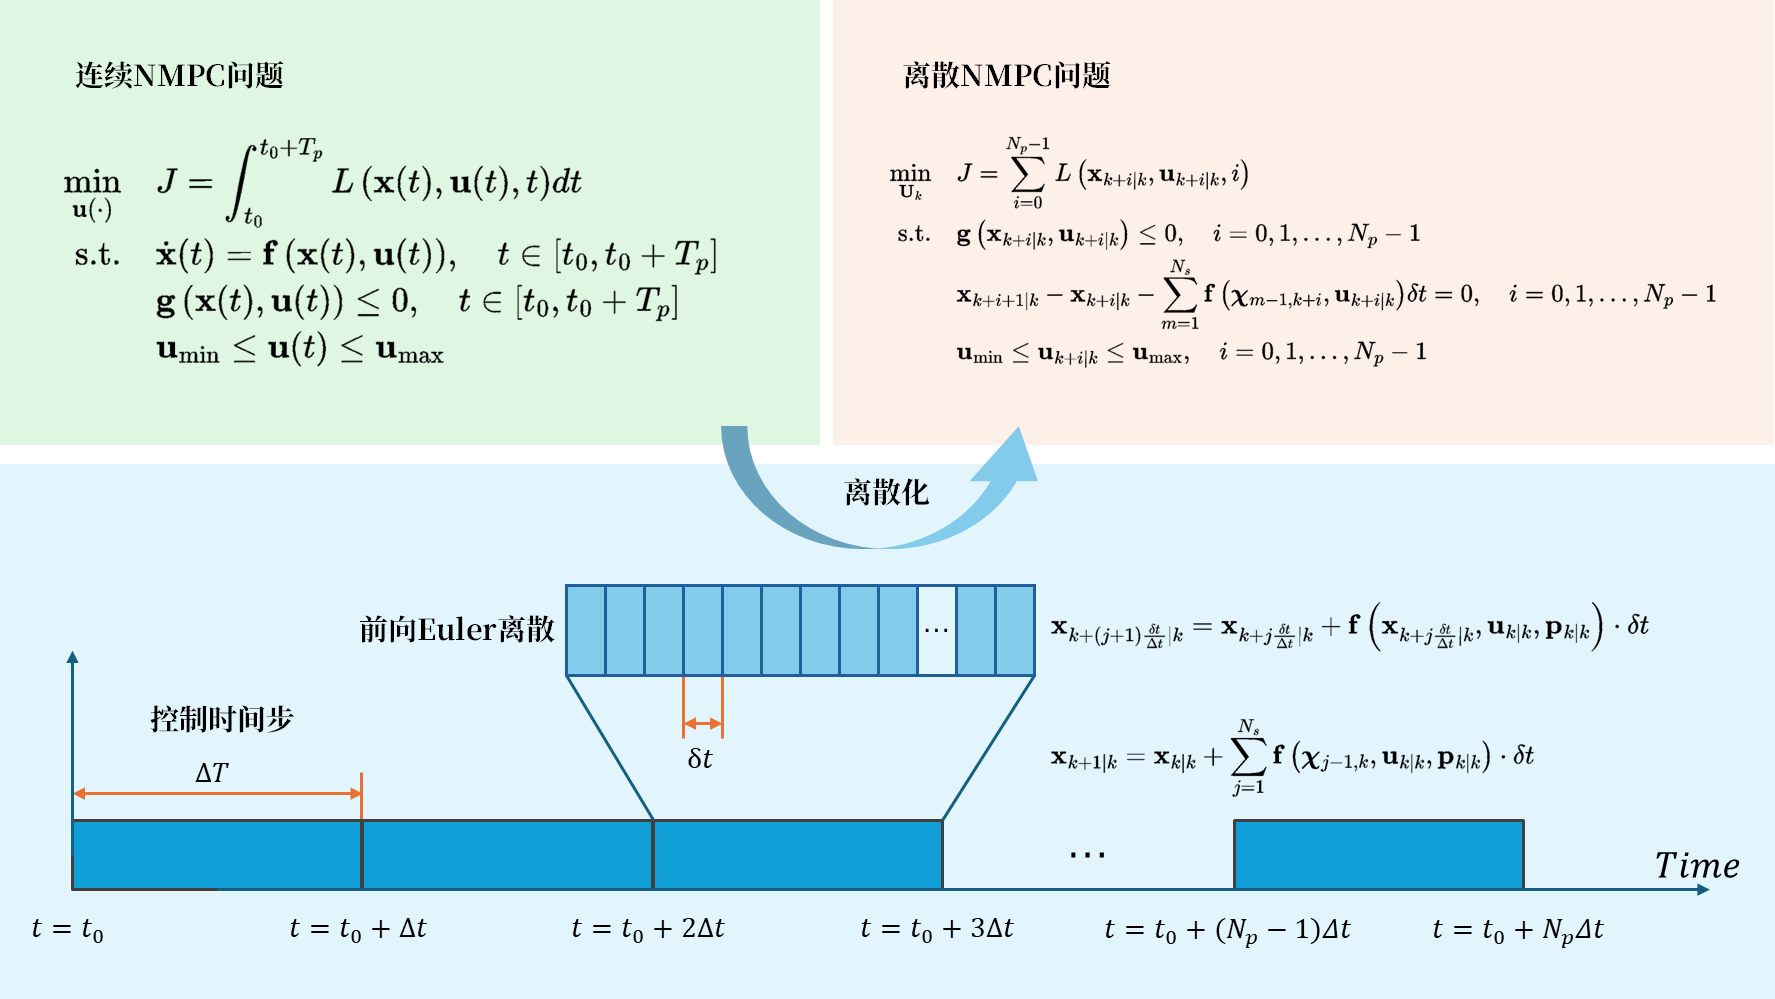
\includegraphics[width=0.95\textwidth]{figures/dnmpc.png}
  \caption{NMPC离散化过程示意图}
  \label{fig:time_scales}
\end{figure}

在当前时刻$k$的离散NMPC优化问题为：

\begin{align}
  \min_{\mathbf{U}_k} \quad & \mathcal{L} = \sum_{i=0}^{N_p-1} \Bigg[ \lambda_{track}\left(P_{total,k+i|k} - P_{ref,k+i}\right)^2 + \lambda_{temp}\sum_{j=1}^{N}\left(T_{s,j,k+i|k} - T_{ref}\right)^2 \nonumber \\
  & \quad + \lambda_I \sum_{j=1}^{N}\left(I_{j,k+i|k} - I_{j,k+i-1|k}\right)^2 + \lambda_{lye} \sum_{j=1}^{N}v_{lye,j,k+i|k}^2 + \lambda_c v_{c,k+i|k}^2 \Bigg] \\
  \text{s.t.} \quad & \mathbf{g}\left(\mathbf{x}_{k+i|k}, \mathbf{u}_{k+i|k}\right) \leq 0, \quad i = 0, 1, \ldots, N_p-1 \\
  & \mathbf{x}_{k+i+1|k} - \mathbf{x}_{k+i|k} - \sum_{m=1}^{N_s} \mathbf{f}\left(\boldsymbol{\chi}_{m-1,k+i}, \mathbf{u}_{k+i|k}\right) \delta t = 0, \quad i = 0, 1, \ldots, N_p-1
\end{align}

其中优化变量为控制序列：
\begin{equation}
  \mathbf{U}_k = \left\{\mathbf{u}_{k|k}, \mathbf{u}_{k+1|k}, \ldots, \mathbf{u}_{k+N_p-1|k}\right\}
\end{equation}

每个控制向量包含以下分量：
\begin{equation}
  \mathbf{u}_{k+i|k} = \left[I_{1,k+i|k}, \ldots, I_{N,k+i|k}, v_{lye,1,k+i|k}, \ldots, v_{lye,N,k+i|k}, v_{c,k+i|k}\right]^\top
\end{equation}

不等式约束$\mathbf{g}(\cdot) \leq 0$包括：
\begin{itemize}
  \item 温度约束：$T_{min} \leq T_{s,j,k+i|k} \leq T_{max}, \quad \forall j = 1, \ldots, N$
  \item 电压约束：$U_{cell,j,k+i|k} \leq U_{cell,max}$
  \item HTO约束：$\mathrm{HTO}_{k+i|k} \leq \mathrm{HTO}_{\mathrm{max}}$
  \item 功率约束：$P_{stack,j,k+i|k} \leq P_{stack,max}$
\end{itemize}

\subsubsection{NMPC求解实现}

NMPC控制器借助CasADi符号计算框架建立优化模型，并由IPOPT求解器进行数值求解。关键实现细节包括：

\begin{itemize}
  \item \textbf{子步进}：每个控制周期内使用$N_s$个仿真子步（步长$\delta t$）确保ODE数值积分稳定性
  \item \textbf{Warm-starting}：利用上一时刻的解作为初始猜测，加速收敛
  \item \textbf{稀疏雅可比}：利用CasADi自动微分生成稀疏雅可比矩阵，提高大规模优化问题求解效率
\end{itemize}

NMPC虽然能够获得高质量的优化控制序列，但其单次求解耗时约17.6~s，难以满足AWE系统的实时控制需求，且存在局部最优风险与参数调节复杂等问题。因此，本文将其作为离线专家控制器，用于生成训练数据，而非直接在线部署。

\subsection{专家数据生成与预处理}

\subsubsection{数据生成流程}

专家数据集通过两类互补的功率轨迹生成，以确保覆盖真实运行场景与极端扰动工况。

\textbf{第一类：风电功率轨迹}。
采用真实风电场出力曲线作为功率参考，反映AWE系统在实际可再生能源波动场景下的跟踪需求。
风电数据代表了真实运行环境，但功率变化相对连续，系统普遍处于跟踪误差较小的稳态附近。

\textbf{第二类：带噪声阶跃实验数据}。
为补充风电数据难以覆盖的大误差场景，设计多平台阶跃功率信号并叠加随机噪声，人为制造功率骤升、骤降与宽频扰动。
这类实验数据能够扩张专家数据集的状态-动作空间覆盖范围，补充NMPC在较大跟踪误差和温度偏差下的控制策略表现，使学习得到的策略具备更强的鲁棒性。

两类数据互为补充：风电数据保证策略在真实场景下的适用性，带噪声阶跃数据则强化策略在非稳态与极端工况下的泛化能力。

在每个控制周期$k$，以系统当前状态$\mathbf{x}_k$、上一时刻控制输入$\mathbf{u}_{k-1}$和参考功率序列$\{P_{ref,k},\ldots,P_{ref,k+N_p-1}\}$为输入，求解NMPC得到最优控制序列$\mathbf{U}_k^\star$。
将首步控制$\mathbf{u}_k^\star$施加到多时间尺度仿真器，在该周期内通过$N_s$个子步对连续动力学数值积分，得到下一周期状态$\mathbf{x}_{k+1}$。
重复上述过程直至完成整段功率轨迹的闭环仿真。NMPC专家数据生成的完整流程如算法~\ref{algo:expert_data_generation} 所示。

\begin{algorithm}[htb]
  \caption{NMPC专家数据生成}
  \label{algo:expert_data_generation}
  \SetAlgoLined
  \KwIn{功率轨迹集合$\{P_{ref}^{(m)}\}_{m=1}^M$，初始状态分布$p(\mathbf{x}_0)$}
  \KwOut{专家数据集$\mathcal{D}$}
  初始化：$\mathcal{D} \leftarrow \emptyset$\\
  \For{每段功率轨迹$m = 1, \ldots, M$}{
    从$p(\mathbf{x}_0)$采样初始状态$\mathbf{x}_0^{(m)}$\\
    \For{每个控制周期$k = 0, \ldots, K-1$}{
      构造功率计划$P_{ref,k:k+N_p-1}^{(m)}$\\
      求解NMPC优化问题，得到最优控制序列$\mathbf{U}_k^\star$\\
      \eIf{NMPC收敛}{
        记录专家样本：$\mathcal{D} \leftarrow \mathcal{D} \cup \{(\mathbf{x}_k, \mathbf{u}_{k-1}, P_{ref,k:k+N_p-1}^{(m)}, \mathbf{u}_k^\star)\}$\\
        执行首步控制$\mathbf{u}_k^\star$，仿真推进至$\mathbf{x}_{k+1}$\\
      }{
        跳过当前样本或采用上一时刻可行解回退\\
      }
    }
  }
  对$\mathcal{D}$进行归一化与训练/测试集划分\\
  \Return{$\mathcal{D}$}
\end{algorithm}

生成过程中记录样本：
\begin{equation}
  \mathcal{D} = \left\{(\mathbf{o}_k, \mathbf{u}_k^\star)\right\}_{k=0}^{K-1}, \quad \mathbf{o}_k = [\mathbf{x}_k, \mathbf{u}_{k-1}, P_{ref,k:k+N_p-1}]
\end{equation}
其中$\mathbf{o}_k$为策略条件输入，包含当前状态、上一时刻控制输入与未来$N_p$步的功率计划，$\mathbf{u}_k^\star$为NMPC给出的专家动作。

\subsubsection{场景覆盖与数据质量控制}

为增强数据集的代表性，专家数据生成覆盖多段功率轨迹与多组初始条件。
每条轨迹开始时，对关键状态（如各槽温度、分离器状态量）进行扰动初始化，以覆盖不同热态与杂质累积水平。
为保证样本质量，若NMPC在个别时刻未能收敛，则跳过该时刻的样本或采用上一时刻可行解作为回退控制，以避免引入明显的异常标签。

\subsubsection{数据格式与预处理}

训练数据以控制周期为采样间隔，输入为$\mathbf{o}_k$，监督标签为$\mathbf{u}_k^\star$。
对各维状态与控制量采用按维线性归一化或标准化处理，使不同量纲的变量在网络训练中具有可比尺度。
数据集按轨迹划分为训练集与测试集，以避免同一条闭环轨迹在不同划分间造成信息泄漏。

\section{TCN Diffusion离线学习策略生成器}

\subsection{扩散模型策略}

在专家数据集构建完成后，需设计一个能够学习该数据分布并生成高质量控制动作的策略网络。与传统回归方法输出单点估计不同，生成模型通过建模动作的条件分布，可在推理阶段采样多条候选轨迹，为在线优化提供丰富的动作空间。去噪扩散概率模型（Denoising Diffusion Probabilistic Model, DDPM）以其训练稳定、生成样本质量高、条件生成灵活等特点，被选为本文策略网络的基础框架。以下从扩散过程的数学原理出发，依次阐述前向加噪、反向去噪、网络训练与推理采样四个核心环节，并说明各环节在四槽AWE控制任务中的具体作用。

DDPM包含前向与反向两个对偶的马尔可夫过程。前向过程从原始数据$\mathbf{x}_0$出发，通过重参数化技巧在任意时间步$t$直接采样加噪状态：
\begin{equation}
  \mathbf{x}_t = \sqrt{\bar{\alpha}_t}\mathbf{x}_0 + \sqrt{1-\bar{\alpha}_t}\boldsymbol{\epsilon}, \quad \boldsymbol{\epsilon} \sim \mathcal{N}(0, \mathbf{I})
\end{equation}
其中$\bar{\alpha}_t = \prod_{s=1}^{t}(1-\beta_s)$，$\beta_t$为方差调度参数。当$T$足够大时，$\mathbf{x}_T$近似服从标准正态分布。在AWE控制任务中，该前向过程对应于对专家最优动作施加渐进扰动，使网络学习在不同噪声水平下恢复高质量控制决策的能力。

反向过程则通过神经网络$\boldsymbol{\epsilon}_\theta(\mathbf{x}_t, t, c)$从噪声中逐步恢复数据，其中$c$为条件信息（如系统状态和功率计划）。直接预测原始数据较为困难，而预测噪声更具效率，因此去噪均值由噪声预测结果给出：
\begin{equation}
  \boldsymbol{\mu}_\theta(\mathbf{x}_t, t) = \frac{1}{\sqrt{\alpha_t}}\left(\mathbf{x}_t - \frac{1-\alpha_t}{\sqrt{1-\bar{\alpha}_t}}\boldsymbol{\epsilon}_\theta(\mathbf{x}_t, t, c)\right)
\end{equation}
反向过程使网络能够学习专家最优动作的条件分布，而非单点估计，从而为在线优化提供丰富的候选动作空间。

网络训练采用噪声预测的均方误差作为目标函数：
\begin{equation}
  \mathcal{L} = \mathbb{E}_{t, \mathbf{x}_0, \boldsymbol{\epsilon}} \left[ \| \boldsymbol{\epsilon} - \boldsymbol{\epsilon}_\theta(\mathbf{x}_t, t, c) \|^2 \right]
\end{equation}
该损失驱使网络准确预测施加在专家动作上的噪声，从而隐式学习不同工况下的最优控制分布。具体训练流程如算法~\ref{algo:diffusion_training} 所示：在每个迭代中随机采样专家批次、时间步与高斯噪声，计算加噪样本后输入噪声预测网络，以均方误差进行梯度下降更新。该流程无需对完整扩散链显式建模，仅通过单步噪声预测即可有效学习专家策略的条件分布。

\begin{algorithm}[htb]
  \caption{TCN Diffusion训练流程}
  \label{algo:diffusion_training}
  \SetAlgoLined
  \KwIn{专家数据集$\mathcal{D}$，扩散步数$T$，批大小$B$，学习率$\eta$，训练轮数$E$}
  \KwOut{训练好的噪声预测网络参数$\theta$}
  对$\mathcal{D}$中的状态与动作进行Min-Max归一化\\
  初始化网络参数$\theta$\\
  \For{$epoch = 1, \ldots, E$}{
    随机打乱数据集$\mathcal{D}$\\
    \For{每个批次$\{(\mathbf{x}_0^{(i)}, c^{(i)})\}_{i=1}^B \subset \mathcal{D}$}{
      采样时间步$t^{(i)} \sim \mathcal{U}(\{1, \ldots, T\})$\\
      采样噪声$\boldsymbol{\epsilon}^{(i)} \sim \mathcal{N}(0, \mathbf{I})$\\
      计算加噪样本：$\mathbf{x}_{t^{(i)}}^{(i)} = \sqrt{\bar{\alpha}_{t^{(i)}}}\mathbf{x}_0^{(i)} + \sqrt{1-\bar{\alpha}_{t^{(i)}}}\boldsymbol{\epsilon}^{(i)}$\\
      预测噪声：$\hat{\boldsymbol{\epsilon}}^{(i)} = \boldsymbol{\epsilon}_\theta(\mathbf{x}_{t^{(i)}}^{(i)}, t^{(i)}, c^{(i)})$\\
      计算损失：$\mathcal{L} = \frac{1}{B}\sum_{i=1}^B \|\boldsymbol{\epsilon}^{(i)} - \hat{\boldsymbol{\epsilon}}^{(i)}\|^2$\\
      梯度下降更新：$\theta \leftarrow \theta - \eta \nabla_\theta \mathcal{L}$\\
    }
  }
  \Return{$\theta$}
\end{algorithm}

训练完成后，从标准正态分布采样初始噪声$\mathbf{x}_T$，迭代执行去噪步骤：
\begin{equation}
  \mathbf{x}_{t-1} = \frac{1}{\sqrt{\alpha_t}}\left(\mathbf{x}_t - \frac{1-\alpha_t}{\sqrt{1-\bar{\alpha}_t}}\boldsymbol{\epsilon}_\theta(\mathbf{x}_t, t, c)\right) + \sqrt{\beta_t}\mathbf{z}
\end{equation}
其中$\mathbf{z} \sim \mathcal{N}(0, \mathbf{I})$。经过$T$步迭代后得到生成的动作序列$\mathbf{x}_0$。在AWE在线控制中，该推理过程在每个控制周期执行，从当前状态和功率计划出发，快速生成多条候选动作序列供后续评估与选择。

扩散模型在控制任务中具有三项核心优势：一是能够建模动作的多峰分布，突破回归方法的单点估计局限；二是生成的序列平滑且符合物理约束；三是通过条件信息$c$实现上下文相关的动作生成，并可在推理阶段灵活调整采样数量以权衡计算开销与控制品质。

在预测控制框架中，策略网络以当前状态和未来功率计划为条件，生成候选动作序列$\mathbf{a}_{t:t+N_p} \sim \pi_\theta(\cdot | \mathbf{x}_t, P_{ref,t:t+N_p})$。通过并行采样与代价评估选取最优序列，扩散模型在动作空间中实现了隐式在线优化。在线部署阶段的推理架构如图~\ref{fig:framework} 所示，完整示意了从条件输入经扩散生成、代价评估、安全修正到闭环执行的完整数据流。

\begin{figure}[!htbp]
  \centering
  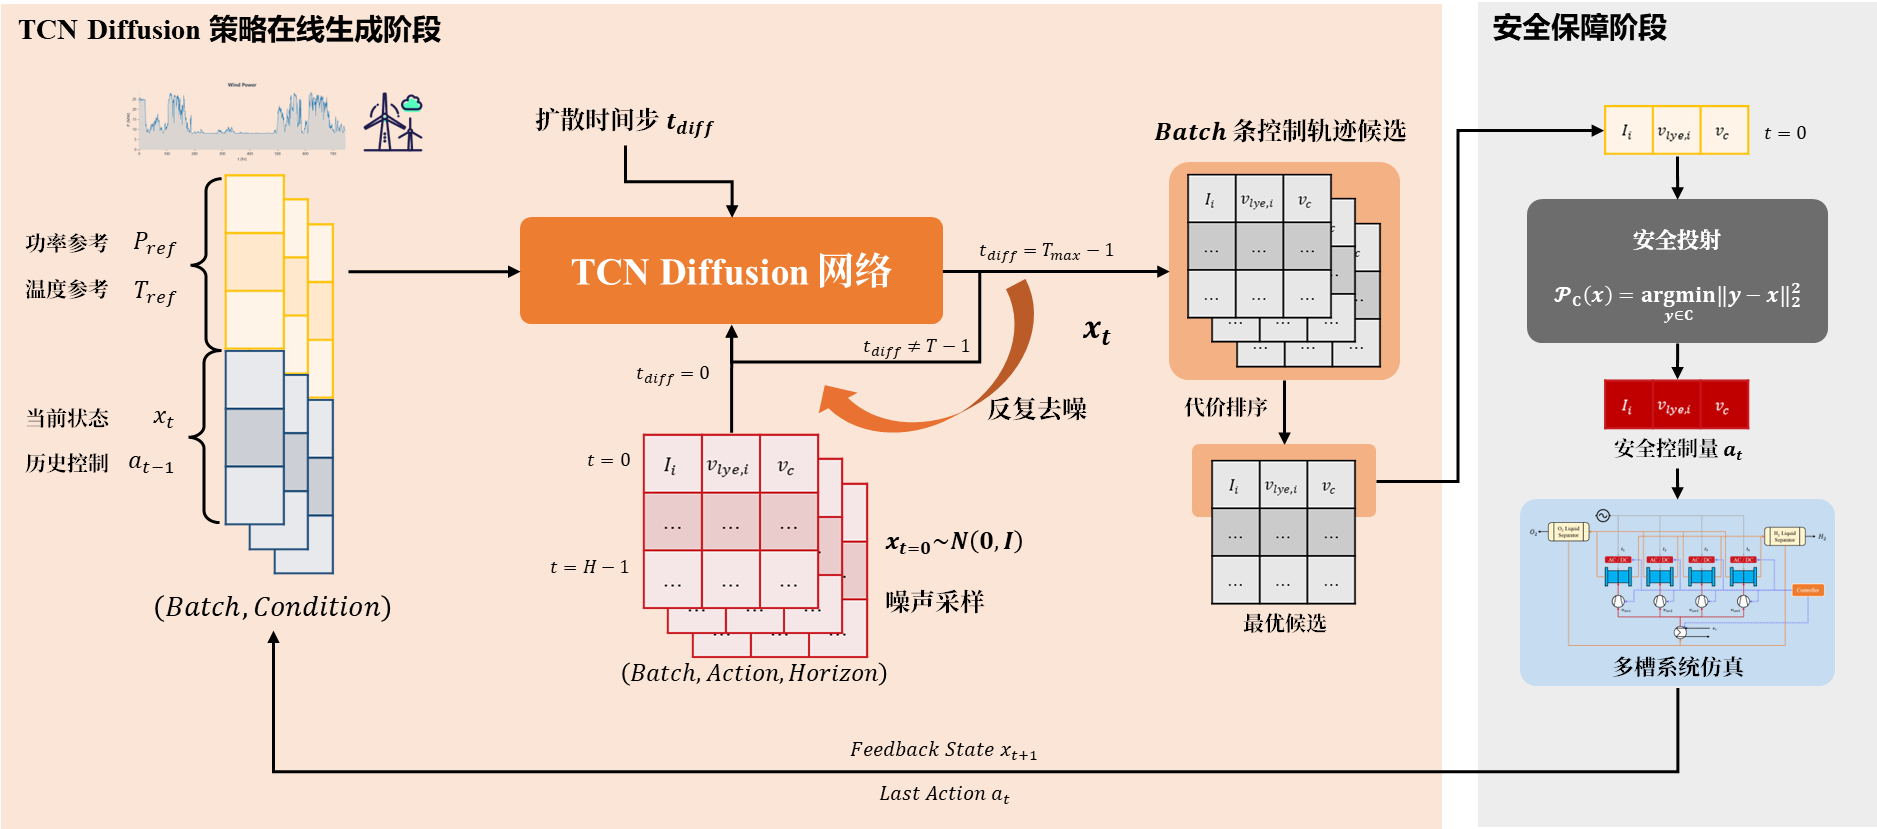
\includegraphics[width=0.98\textwidth]{figures/control_structure.png}
  \caption{基于TCN Diffusion的安全学习控制框架}
  \label{fig:framework}
\end{figure}

\subsection{网络架构}

基于上述扩散策略，策略生成器的网络设计需同时满足两项要求：一是对电解系统长时序动态的有效建模，二是在线推理的实时性约束。
本节从主干网络选择与条件编码机制两方面阐述实现方案，并说明网络架构如何与推理流程协同以逼近优化级控制品质。

时序卷积网络（Temporal Convolutional Network, TCN）被选为噪声预测网络的主干结构。
与循环神经网络相比，TCN的因果卷积结构保证了时序因果性，其空洞卷积机制使感受野随网络深度指数级扩展，从而以较少的层数捕获电解系统热惯性、气体传输等长程动态依赖。
同时，TCN摒弃了循环结构中的时序依赖计算，训练与推理过程均可完全并行化，显著提升了计算效率。

条件编码方面，当前系统状态、功率计划与历史动作经特征投影后，与噪声输入及时间步嵌入共同注入TCN主干。
图~\ref{fig:network_arch} 展示了该网络的整体架构。

% network_structure.png TCN Diffusion网络架构图
\begin{figure}[!htbp]
  \centering
  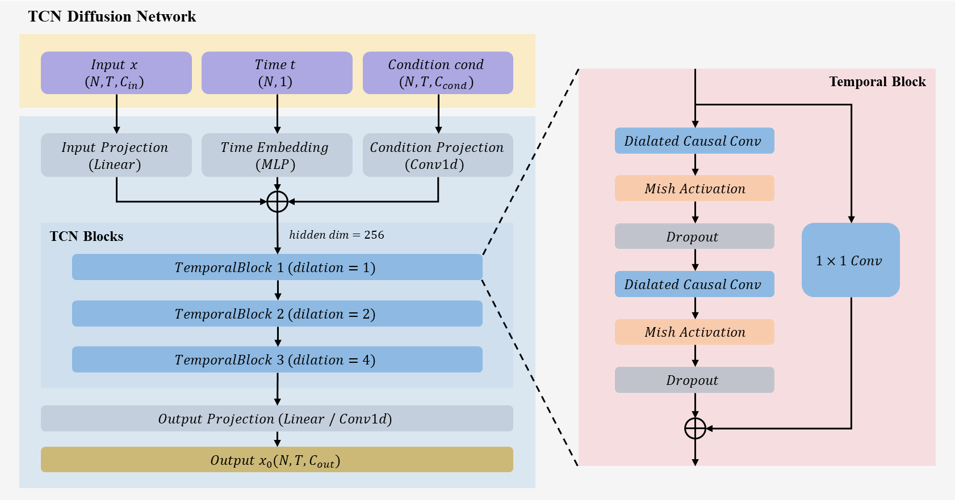
\includegraphics[width=0.98\textwidth]{figures/network_structure.png}
  \caption{TCN Diffusion网络架构图}
  \label{fig:network_arch}
\end{figure}

在推理阶段，网络首先从标准正态分布采样初始噪声，经去噪迭代生成$K$条候选动作序列；
随后通过物理模型推演评估各序列的综合代价，并直接选取代价最低的序列作为控制输出。
该生成-评估-选择的流程在计算结构上等价于一次并行的、基于物理模型的在线优化：
无需迭代求解高维非线性规划，而是以$K$次前向仿真的开销换取接近优化求解的控制品质。
此外，候选轨迹的评估过程可充分利用GPU并行计算能力批量执行，进一步压缩在线决策时间。
上述控制流程如算法~\ref{algo:generative_control} 所示。

\begin{algorithm}[htb]
  \caption{生成模型控制策略}
  \label{algo:generative_control}
  \SetAlgoLined
  \KwIn{当前状态$\mathbf{x}_t$，功率计划$P_{ref}$，策略模型$\pi_\theta$，采样数$K$}
  \KwOut{控制动作$\mathbf{a}_t$}

  % 采样候选序列
  采样$K$条候选动作序列$\{\mathbf{a}^{(i)}\}_{i=1}^K \sim \pi_\theta(\mathbf{x}_t, P_{ref})$

  % 评估每条序列
  \For{$i = 1, \ldots, K$}{
    使用物理模型推演轨迹$\boldsymbol{\tau}^{(i)}$

    计算综合代价：
    $\mathcal{L}^{(i)} = \lambda_{track}\ell_{track}^{(i)} + \lambda_{temp}\ell_{temp}^{(i)} + \lambda_{I}\ell_{I}^{(i)} + \lambda_{lye}\ell_{lye}^{(i)} + \lambda_{c}\ell_{c}^{(i)}$
  }

  % 选取最优序列
  选取代价最小的动作索引：$i^* = \arg\min_i \mathcal{L}^{(i)}$

  提取首步动作：$\mathbf{a}_t = \mathbf{a}^{(i^*)}_0$

  \Return{$\mathbf{a}_t$}
\end{algorithm}

\section{安全约束保证机制}

控制障碍函数（Control Barrier Function, CBF）从李导数出发，为安全约束提供了可严格证明的前向不变性框架~\cite{Ames2019CBF}。
本节针对AWE系统的HTO非仿射约束与温度约束，建立多重CBF联合安全框架：首先回顾CBF基本概念（3.4.1），随后分别推导HTO约束（3.4.2）与温度约束（3.4.3）的CBF形式，最后将两类约束统一为多重CBF联合优化问题并给出求解算法（3.4.4）。

\subsection{CBF基本概念}

在将CBF理论应用于AWE系统之前，需先明确一阶CBF的数学定义与适用条件。一阶CBF要求控制输入直接出现在约束函数的一阶导数中，适用于控制灵敏度充足的场景。

考虑一般非线性控制系统$\dot{\mathbf{x}} = \mathbf{f}(\mathbf{x}, \mathbf{u})$，其中$\mathbf{x}\in\mathbb{R}^n$，$\mathbf{u}\in\mathcal{U}\subset\mathbb{R}^m$。设安全集$\mathcal{C}$定义为：
\begin{equation}
  \mathcal{C} = \left\{ \mathbf{x}\in\mathbb{R}^n \mid h(\mathbf{x}) \ge 0 \right\}
\end{equation}
其中$h: \mathbb{R}^n \to \mathbb{R}$为连续可微函数。若存在类$\mathcal{K}$函数$\alpha(\cdot)$使得对所有$\mathbf{x}\in\mathcal{C}$有：
\begin{equation}
  \sup_{\mathbf{u}\in\mathcal{U}} \left[ \frac{\partial h}{\partial \mathbf{x}} \mathbf{f}(\mathbf{x}, \mathbf{u}) \right] \ge -\alpha(h(\mathbf{x}))
\end{equation}
则称$h$为控制障碍函数。取$\alpha(h) = \gamma_{CBF} h$（$\gamma_{CBF}>0$），得到广泛采用的指数型CBF条件：
\begin{equation}
  \dot{h}(\mathbf{x}, \mathbf{u}) + \gamma_{CBF} h(\mathbf{x}) \ge 0
\label{eq:cbf_condition}
\end{equation}
式~\eqref{eq:cbf_condition} 保证了安全集$\mathcal{C}$的前向不变性：若$\mathbf{x}(0)\in\mathcal{C}$，则对所有$t\ge 0$有$\mathbf{x}(t)\in\mathcal{C}$。

对于AWE系统，HTO约束与温度约束的控制输入均直接出现在一阶导数中（相对度为1），满足标准CBF可解性要求，因此均采用一阶CBF处理。通过合理选取CBF增益参数$\gamma_{CBF}$并在优化目标中引入控制量参考跟踪权重，可在保证安全性的同时获得平滑的控制响应。

\subsection{HTO约束的CBF推导}

HTO约束是AWE系统安全控制的核心难点之一：其动态涉及气液分离器温度与气相氢含量的耦合，且电流通过法拉第效率以非仿射形式进入约束导数。本节推导HTO约束的一阶CBF李导数形式，为后续联合优化提供可计算的约束条件。

以HTO约束为例，推导其CBF李导数。根据理想气体状态方程$PV=nRT$，气相中氢气的体积百分比为：
\begin{equation}
  HTO_{pct} = \frac{n_{gas} \cdot R \cdot T_{sep}}{P_{sys} \cdot V_{sep,gas}} \times 100\%
\end{equation}
工程安全要求$\mathrm{HTO}_{\mathrm{pct}} \le 2\%$。定义系统常数：
\begin{equation}
  K_{HTO} = \frac{R}{P_{sys} \cdot V_{sep,gas}}
\end{equation}
为便于李导数推导，以单槽的7维状态向量为分析对象：
\begin{equation}
  \mathbf{x} = [x_1, \dots, x_7]^\top = [T_{s,in}, T_s, T_{sep}, T_{c,out}, n_{H_2,an}, n_{liq}, n_{gas}]^\top
\end{equation}
则HTO约束可写为状态空间形式$K_{HTO} \cdot x_3 \cdot x_7 \le 0.02$，其中$x_3 = T_{sep}$，$x_7 = n_{gas}$。

选取CBF候选函数如式~\eqref{eq:h_hto} 所示，将HTO安全约束显式写为系统状态的函数：
\begin{equation}
  h_{HTO}(\mathbf{x}) = 0.02 - K_{HTO} \cdot x_3 \cdot x_7
\label{eq:h_hto}
\end{equation}
上述CBF函数的梯度向量如下：
\begin{equation}
  \nabla h_{HTO} = \left[ 0,\ 0,\ -K_{HTO} \cdot x_7,\ 0,\ 0,\ 0,\ -K_{HTO} \cdot x_3 \right]
\end{equation}

CBF的时间导数由链式法则给出：
\begin{equation}
  \dot{h}_{HTO} = \nabla h_{HTO} \cdot f(\mathbf{x}, \mathbf{u}) = -K_{HTO} \cdot \left( x_7 \dot{x}_3 + x_3 \dot{x}_7 \right)
\label{eq:h_hto_dot_chain}
\end{equation}

分离器温度动态$\dot{x}_3$为：
\begin{equation}
  \dot{x}_3 = \frac{1}{C_{sep}}\left[ c_{lye}\rho_{lye} u_2 (x_2 - x_3) - Q_{sep,diss}(x_3) \right]
\end{equation}
其中$Q_{sep,diss}(x_3) = h_{sep}(x_3 - T_{amb})$为分离器热耗散功率。

气相氢气动态$\dot{x}_7$为：
\begin{equation}
  \dot{x}_7 = \frac{x_6}{\tau_{sep}} - \frac{R \cdot x_3 \cdot x_7 \cdot N_{cell} \cdot u_1 \cdot \eta_F(u_1, x_2)}{4F \cdot P_{sys} \cdot V_{sep,gas}}
\end{equation}
其中关键的非仿射耦合项为$u_1 \cdot \eta_F(u_1, x_2)$，法拉第效率：
\begin{equation}
  \eta_F(I, T_s) = \frac{I^2}{f_1(T_s) + I^2} \cdot f_2(T_s)
\end{equation}
将$\dot{x}_3$与$\dot{x}_7$代入式~\eqref{eq:h_hto_dot_chain} 后整理，可得控制仿射与非仿射混合形式：
\begin{equation}
  \dot{h}_{HTO}(\mathbf{x}, \mathbf{u}) = \underbrace{\gamma(\mathbf{x}) \cdot u_1 \cdot \eta_F(u_1, x_2)}_{\text{电流控制（非仿射）}} - \underbrace{\beta(\mathbf{x}) \cdot u_2}_{\text{流量控制（仿射）}} + \underbrace{\phi(\mathbf{x})}_{\text{纯状态漂移}}
\label{eq:h_hto_expanded}
\end{equation}

其中各系数定义如下：
\begin{align}
  \gamma(\mathbf{x}) &= \frac{R^2 \cdot N_{cell} \cdot x_3^2 \cdot x_7}{4F \cdot P_{sys}^2 \cdot V_{sep,gas}^2} > 0 \quad (\text{当 } x_3, x_7 > 0) \\
  \beta(\mathbf{x}) &= \frac{K_{HTO} \cdot c_{lye} \cdot \rho_{lye} \cdot x_7 \cdot (x_2 - x_3)}{C_{sep}} \\
  \phi(\mathbf{x}) &= \frac{K_{HTO} \cdot x_7 \cdot Q_{sep,diss}(x_3)}{C_{sep}} - \frac{K_{HTO} \cdot x_3 \cdot x_6}{\tau_{sep}}
\end{align}

由式~\eqref{eq:h_hto_expanded} 可分析各控制动作对$\dot{h}_{HTO}$的影响：
增大电流$u_1$时，由于$\gamma(\mathbf{x})>0$且$\eta_F>0$，$\dot{h}_{HTO}$正向提升，即推动系统远离HTO边界；
增大碱液流速$u_2$的影响取决于$\beta(\mathbf{x})$的符号，若$x_2 > x_3$，增大$u_2$可降低分离器温度从而间接降低HTO；
漂移项$\phi(\mathbf{x})$则反映散热与液相传质的被动影响。

上述分析表明，HTO安全约束对电流与碱液流量的响应方向并非恒定，而是取决于当前状态（尤其是$\beta(\mathbf{x})$的符号）。这进一步说明，仅凭定性经验难以保证安全，必须借助CBF的定量约束条件实现系统性安全控制。

基于式~\eqref{eq:h_hto_expanded} 推导得到的一阶李导数$\dot{h}_{HTO}(\mathbf{x}, \mathbf{u})$，HTO约束的一阶CBF条件为：
\begin{equation}
  \dot{h}_{HTO}(\mathbf{x}, \mathbf{u}) + \gamma_{HTO} \, h_{HTO}(\mathbf{x}) \ge 0
\label{eq:cbf_hto}
\end{equation}
其中$\gamma_{HTO} > 0$为CBF增益参数，决定HTO安全边界的收敛速率。

在实际实现中，采用状态自适应的CBF增益策略：当HTO远离安全边界（$h_{HTO}$较大）时，取较大的$\gamma_{HTO}$以降低保守性，允许系统以更自然的动态运行；当HTO逼近边界（$h_{HTO}$较小）时，自动减小$\gamma_{HTO}$以增强约束强度，确保安全性。该策略通过Sigmoid函数实现平滑切换，避免增益突变导致的控制量抖振。同时，在优化目标中引入控制量参考跟踪权重$u_{\rm weight}$，对电流、碱液流量与冷却水流量分别设置不同的偏离惩罚系数，使CBF在满足安全约束的前提下尽可能贴近参考控制量，从而获得平滑的控制响应。

\subsection{温度约束的CBF推导}

与HTO约束的非仿射特性不同，电解槽温度动态中控制输入（电流与碱液流量）直接出现在一阶导数中，相对度为1，且灵敏度充足。因此，温度上下限约束可直接采用一阶CBF处理，无需引入高阶导数。本节推导温度CBF的李导数形式，并分析电流与流量对温度安全裕度的影响方向。

除HTO约束外，温度上下限同样需要严格满足。选取仅依赖于状态$x_2 = T_s$的CBF候选函数：
\begin{equation}
  \begin{aligned}
    h_1(\mathbf{x}) &= 363.15 - x_2, \\
    h_2(\mathbf{x}) &= x_2 - 293.15
  \end{aligned}
  \label{eq:h_temperature}
\end{equation}
其中$h_1$对应温度上限（$90^\circ$C），$h_2$对应温度下限（$20^\circ$C）。

$h_1$的梯度向量仅对$x_2$有非零偏导：
\begin{equation}
  \nabla h_1 = \left[ 0,\ -1,\ 0,\ 0,\ 0,\ 0,\ 0 \right]
\end{equation}

根据链式法则，其时间导数为：
\begin{equation}
  \dot{h}_1 = \nabla h_1 \cdot f(\mathbf{x}, \mathbf{u}) = -\dot{x}_2 = -\dot{T}_s
\end{equation}

将电解槽热平衡动态$\dot{x}_2$代入并展开整理，可得控制仿射与非仿射混合形式：
\begin{equation}
  \dot{h}_1(\mathbf{x}, \mathbf{u}) = \underbrace{\alpha(\mathbf{x}, u_1)}_{\text{电流控制（非仿射）}} + \underbrace{\beta(\mathbf{x}) \cdot u_2}_{\text{流量控制（仿射）}} + \underbrace{\psi(\mathbf{x})}_{\text{纯状态漂移}}
  \label{eq:h1_dot}
\end{equation}

其中各系数定义如下：
\begin{align}
  \alpha(\mathbf{x}, u_1) &= -\frac{N_{cell}}{C_s} u_1 \left[ U_{cell}(u_1, x_2) - \eta_F(u_1, x_2) U_{th} \right] \\
  \beta(\mathbf{x}) &= \frac{c_{lye} \cdot \rho_{lye} \cdot (x_2 - x_1)}{C_s} \\
  \psi(\mathbf{x}) &= \frac{\sigma_s(x_2 - T_{am}) + \epsilon_s \sigma_b A_{stack}(x_2^4 - T_{am}^4)}{C_s}
\end{align}

$\alpha(\mathbf{x}, u_1)$关于电流$u_1$呈非仿射关系，包含$u_1$与电压$U_{cell}$以及法拉第效率$\eta_F$的耦合；
$\beta(\mathbf{x})$为碱液流量$u_2$的仿射系数，其符号由$x_2 - x_1$决定；
$\psi(\mathbf{x})$仅依赖于状态$x_2 = T_s$，反映对流与辐射散热的被动影响，与控制输入无关。
由于$U_{cell} > \eta_F U_{th}$，产热功率恒为正，故$\alpha(\mathbf{x}, u_1) < 0$，意味着增大电流会使$\dot{h}_1$减小（温度上升，安全裕度降低）。
当$x_2 > x_1$时，$\beta(\mathbf{x}) > 0$，增大$u_2$可使$\dot{h}_1$增大（带走更多热量，提升安全裕度）。由此可见，温度安全裕度与电流呈负相关、与碱液流量呈正相关（当$x_2 > x_1$时），这与工程直觉一致，也为后续联合优化中各控制量的协调方向提供了先验依据。

类似地，$h_2$的梯度为$\nabla h_2 = [0, 1, 0, 0, 0, 0, 0]$，时间导数为：
\begin{equation}
  \dot{h}_2(\mathbf{x}, \mathbf{u}) = \underbrace{-\alpha(\mathbf{x}, u_1)}_{\text{电流控制（非仿射）}} - \underbrace{\beta(\mathbf{x}) \cdot u_2}_{\text{流量控制（仿射）}} - \underbrace{\psi(\mathbf{x})}_{\text{纯状态漂移}} = -\dot{h}_1(\mathbf{x}, \mathbf{u})
  \label{eq:h2_dot}
\end{equation}

温度约束的CBF条件分别为：
\begin{equation}
  \begin{aligned}
    \dot{h}_1(\mathbf{x}, \mathbf{u}) + \gamma_1 h_1(\mathbf{x}) &\ge 0, \\
    \dot{h}_2(\mathbf{x}, \mathbf{u}) + \gamma_2 h_2(\mathbf{x}) &\ge 0
  \end{aligned}
  \label{eq:cbf_temperature}
\end{equation}

式中$\gamma_1, \gamma_2 > 0$决定温度安全边界的指数收敛速率：取值越大，系统趋近安全边界时被"推回"的力道越强，但过大可能导致控制量饱和。工程上需在响应速度与控制平滑性之间权衡。

\subsection{多重CBF联合约束}

上述两小节分别推导了温度安全约束与HTO安全约束的CBF条件。然而，在实际电解槽运行中，温度超限与氢氧纯度恶化并非独立事件——高温会降低法拉第效率从而加速HTO上升，而HTO异常又往往伴随反应热功率变化。因此，必须将两类约束统一纳入同一个安全滤波器，形成多重CBF联合约束框架，确保任何工况下系统均不触及安全边界。

定义如下多重CBF候选函数集合：
\begin{equation}
  \begin{array}{ll}
    h_1(\mathbf{x}) = 363.15 - x_2, & \text{（温度上限，90$^\circ$C，一阶CBF）} \\
    h_2(\mathbf{x}) = x_2 - 293.15, & \text{（温度下限，20$^\circ$C，一阶CBF）} \\
    h_3(\mathbf{x}) = 0.02 - K_{HTO} \cdot x_3 \cdot x_7, & \text{（HTO上限，一阶CBF）}
  \end{array}
  \label{eq:multi_cbf_set}
\end{equation}

温度约束采用一阶CBF条件，因其控制输入直接出现在一阶导数$\dot{h}_1$、$\dot{h}_2$中（见式~\eqref{eq:h1_dot}与式~\eqref{eq:h2_dot}），相对度为1，满足标准CBF可解性要求。HTO约束同样采用一阶CBF条件，通过式~\eqref{eq:h_hto_expanded}中碱液流量的仿射作用以及电流的非仿射耦合，可直接构建控制可解的安全约束。

在每个控制时刻，CBF安全滤波器将上述条件同时作为不等式约束，求解以下优化问题：
\begin{equation}
  \begin{aligned}
    \min_{\mathbf{u}\in\mathcal{U},\,\mathbf{s}\ge 0} \quad & \|\mathbf{u} - \mathbf{u}_{ref}\|_2^2 + \sum_{i=1}^{9} \rho_i s_i^2 \\
    \text{s.t.} \quad & \dot{h}_1(\mathbf{x}, \mathbf{u}) + \gamma_1 h_1(\mathbf{x}) \ge -s_1 \\
    & \dot{h}_2(\mathbf{x}, \mathbf{u}) + \gamma_2 h_2(\mathbf{x}) \ge -s_2 \\
    & \dot{h}_{HTO}(\mathbf{x}, \mathbf{u}) + \gamma_{HTO} h_{HTO}(\mathbf{x}) \ge -s_{HTO} \\
    & \mathbf{u}_{min} \le \mathbf{u} \le \mathbf{u}_{max}
  \end{aligned}
  \label{eq:cbf_optimization}
\end{equation}

式中$\gamma_1, \gamma_2, \gamma_{HTO} > 0$为各CBF的类增益参数，决定安全边界收敛速率，典型取值范围为$0.5 \sim 2.0$。$s_i \ge 0$为各约束对应的松弛变量，用于处理极端工况下约束暂时不可行的情形：当系统状态已越过安全边界或控制输入饱和导致CBF条件无法满足时，松弛变量允许约束以可控幅度临时放宽，避免优化问题无可行解而导致控制器失效。$\rho_i > 0$为松弛惩罚系数，取值越大，对约束违反的惩罚越重，松弛量越趋近于零。本文对所有9条约束统一取$\rho_i = 5000$，该数值在数值实验中表现出良好的折中——既能在可行情形下将松弛量抑制在$10^{-4}$量级以下，又能在极端瞬态（如功率骤降导致的HTO急剧上升）中保持优化问题的数值可行性。由于HTO约束包含$u_1 \cdot \eta_F(u_1, x_2)$这一关于电流的非仿射项，标准的二次规划（QP）方法不再适用，需采用CasADi/IPOPT等通用非线性规划求解器进行数值求解。

CBF安全滤波器的具体执行流程如算法~\ref{algo:cbf_filter} 所示。

\begin{algorithm}[htb]
  \caption{非仿射CBF安全滤波}
  \label{algo:cbf_filter}
  \SetAlgoLined
  \KwIn{当前状态$\mathbf{x}_t$，参考控制量$\mathbf{u}_{ref}$，CBF参数$\{\gamma_i\}_{i=1}^3$}
  \KwOut{安全控制量$\mathbf{u}_t$}
  计算各CBF函数值$\{h_i(\mathbf{x}_t)\}_{i=1}^3$\\
  利用符号自动微分计算李导数$\{\dot{h}_i(\mathbf{x}_t, \mathbf{u})\}_{i=1}^3$\\
  构建联合CBF约束：$\dot{h}_i(\mathbf{x}_t, \mathbf{u}) + \gamma_i h_i(\mathbf{x}_t) \ge 0,\quad i=1,\dots,3$\\
  求解带约束优化问题：\\
  \quad$\mathbf{u}_t = \arg\min_{\mathbf{u}_{min} \le \mathbf{u} \le \mathbf{u}_{max}} \|\mathbf{u} - \mathbf{u}_{ref}\|_2^2$\\
  \qquad s.t. $\dot{h}_i(\mathbf{x}_t, \mathbf{u}) + \gamma_i h_i(\mathbf{x}_t) \ge 0,\quad \forall i$\\
  \If{优化问题不可行}{
    触发可行性回退：$\mathbf{u}_t \leftarrow \mathbf{u}_{min}$ 或采用最近可行解\\
  }
  \Return{$\mathbf{u}_t$}
\end{algorithm}

算法~\ref{algo:cbf_filter} 给出了单次控制周期内的CBF安全滤波流程。然而，该算法仅解决单步约束投影问题，尚未与第 3.3 节建立的生成模型控制策略形成闭环。为此，进一步将CBF安全滤波嵌入扩散模型推理循环：在每个控制周期，先生成模型产生名义控制量，再经CBF滤波修正后施加于系统。完整的闭环安全控制流程如算法~\ref{algo:safe_closed_loop_control} 所示。

\begin{algorithm}[htb]
  \caption{基于扩散模型与安全约束的闭环控制}
  \label{algo:safe_closed_loop_control}
  \SetAlgoLined
  \KwIn{初始状态$\mathbf{x}_0$，功率参考轨迹$\{P_{ref,t}\}$，策略模型$\pi_\theta$，CBF滤波$\mathcal{F}_{CBF}$}
  \KwOut{闭环状态轨迹$\{\mathbf{x}_t\}$与控制轨迹$\{\mathbf{u}_t\}$}
  \For{每个控制周期$t = 0, 1, 2, \ldots$}{
    采样$K$条候选动作序列$\{\mathbf{a}^{(i)}\}_{i=1}^K \sim \pi_\theta(\mathbf{x}_t, P_{ref,t:t+N_p-1})$\\
    \For{$i = 1, \ldots, K$}{
      使用物理模型推演轨迹并计算代价$\mathcal{L}^{(i)}$\\
    }
    选取代价最小的动作作为名义动作$\mathbf{u}_{nom} = \mathbf{a}^{(\arg\min_i \mathcal{L}^{(i)})}_0$\\
    $\mathbf{u}_t \leftarrow \mathcal{F}_{CBF}(\mathbf{u}_{nom}, \mathbf{x}_t)$ \tcp*{CBF安全滤波}
    将$\mathbf{u}_t$施加到多时间尺度仿真器，推进至下一状态$\mathbf{x}_{t+1}$\\
  }
  \Return{$\{\mathbf{x}_t\}, \{\mathbf{u}_t\}$}
\end{algorithm}

综上，本节建立了面向四槽AWE系统的多重CBF联合安全框架：温度约束与HTO约束均采用一阶CBF条件，统一纳入逐时刻非线性约束优化问题，通过CasADi/IPOPT进行数值求解。该框架为生成模型控制策略提供了严格的前向不变性保证，且单次求解时间低于20~ms，满足实时控制要求。
下文将通过闭环仿真实验，验证CBF约束保证机制在四槽AWE系统中的实际控制效果。

\section{实验验证与结果分析}

\subsection{开环验证}

开环验证旨在检验所建立的多槽AWE系统模型能否准确复现真实电解槽在无反馈条件下的控制-响应耦合特性，尤其是电流、碱液流量与冷却水流量对电解槽温度及HTO浓度的跨槽耦合影响。
实验采用第\ref{chap:modeling}章建立的4槽物理仿真模型，状态维度为13维，控制维度为9维，ODE积分采用RK45方法（$dt=0.2$~s），热力学模型包含电化学反应热、对流/辐射散热及换热器LMTD模型，HTO动力学基于Fick扩散、Darcy对流与气液分离器质量平衡。

系统初始状态取热力学稳态解：四槽温度均为77.1$^\circ$C（350.25~K），分离器温度77.0$^\circ$C（350.15~K），换热器出口碱液温度77.0$^\circ$C（350.15~K），冷却水出口温度52.0$^\circ$C（325.15~K），HTO浓度0.458\%，各阳极室与分离器内氢气物质的量由HTO平衡反算确定。
在此基础上，从$t=0$时刻起依次施加5个阶跃扰动，以验证不同控制动作对系统状态的独立影响与耦合效应。动作序列如表~\ref{tab:open_loop_actions}所示。

\begin{table}[!htbp]
  \centering
  \caption{开环动作序列}
  \label{tab:open_loop_actions}
  \begin{tabular}{cp{3.2cm}p{6.5cm}c}
    \toprule
    动作 & 时刻 & 控制变化 & 受影响槽 \\
    \midrule
    Action I & $t=900$~s（15~min） & Stack~1碱液流量：$3.35\times10^{-2}\to2.5\times10^{-2}$~m$^3$/s & 仅槽1 \\
    Action II & $t=1,800$~s（30~min） & Stack~1电流：$7,000\to3,500$~A & 仅槽1 \\
    Action III & $t=2,700$~s（45~min） & Stack~2电流：$7,000\to3,500$~A & 仅槽2 \\
    Action IV & $t=3,600$~s（60~min） & Stack~3电流：$7,000\to3,500$~A & 仅槽3 \\
    Action V & $t=4,500$~s（75~min） & 冷却水流量：$5.0\times10^{-2}\to2.0\times10^{-2}$~m$^3$/s & 全局 \\
    \bottomrule
  \end{tabular}
\end{table}

图~\ref{fig:open_loop_response}展示了开环实验的动态响应曲线。
温度方面，Action I将槽1碱液流量降低后，槽1温度上升（冷却能力减弱），与理论预期一致；Actions II至IV依次降低槽1--3电流后，对应槽温度显著下降（产热减少），分离器温度由77$^\circ$C降至约60$^\circ$C；Action V降低冷却水流量后，所有槽及分离器温度同时回升约5--10$^\circ$C，体现了冷却水作为全局热管理变量的耦合作用。

HTO方面，Action I使HTO轻微下降（碱液流量减少导致携带H$_2$进入分离器的量略减）；Actions II至IV使HTO从0.46\%逐步上升至0.73\%（电流降低导致产氧量减少，气相稀释作用减弱）；Action V使HTO继续小幅上升（温度升高加速H$_2$脱附）。

功率方面，总功率随Actions II至IV阶梯式下降，由约22~MW依次降至约15~MW、12~MW与10~MW；Action V不改变电功率，仅影响热管理。

上述实验结果揭示了多槽AWE系统的三项核心物理规律。其一，MIMO耦合特性显著：单个槽的电流或流量变化不仅影响本槽温度，还通过共享碱液回路和冷却系统影响其他槽与分离器，验证了控制器设计必须考虑多输入多输出特性。其二，热惯性明显：温度对控制动作的响应存在分钟级滞后，而HTO响应更为缓慢（数十分钟级），体现了热力学与传质过程的时间尺度分离。其三，冷却水具有全局调节作用：Action V表明冷却水流量是影响全系统温度的全局变量，其调节可同时改变所有组件的热状态，在控制器设计中需作为关键全局约束处理。

\begin{figure}[!htbp]
  \centering
  \begin{subfigure}{0.31\textwidth}
    \centering
    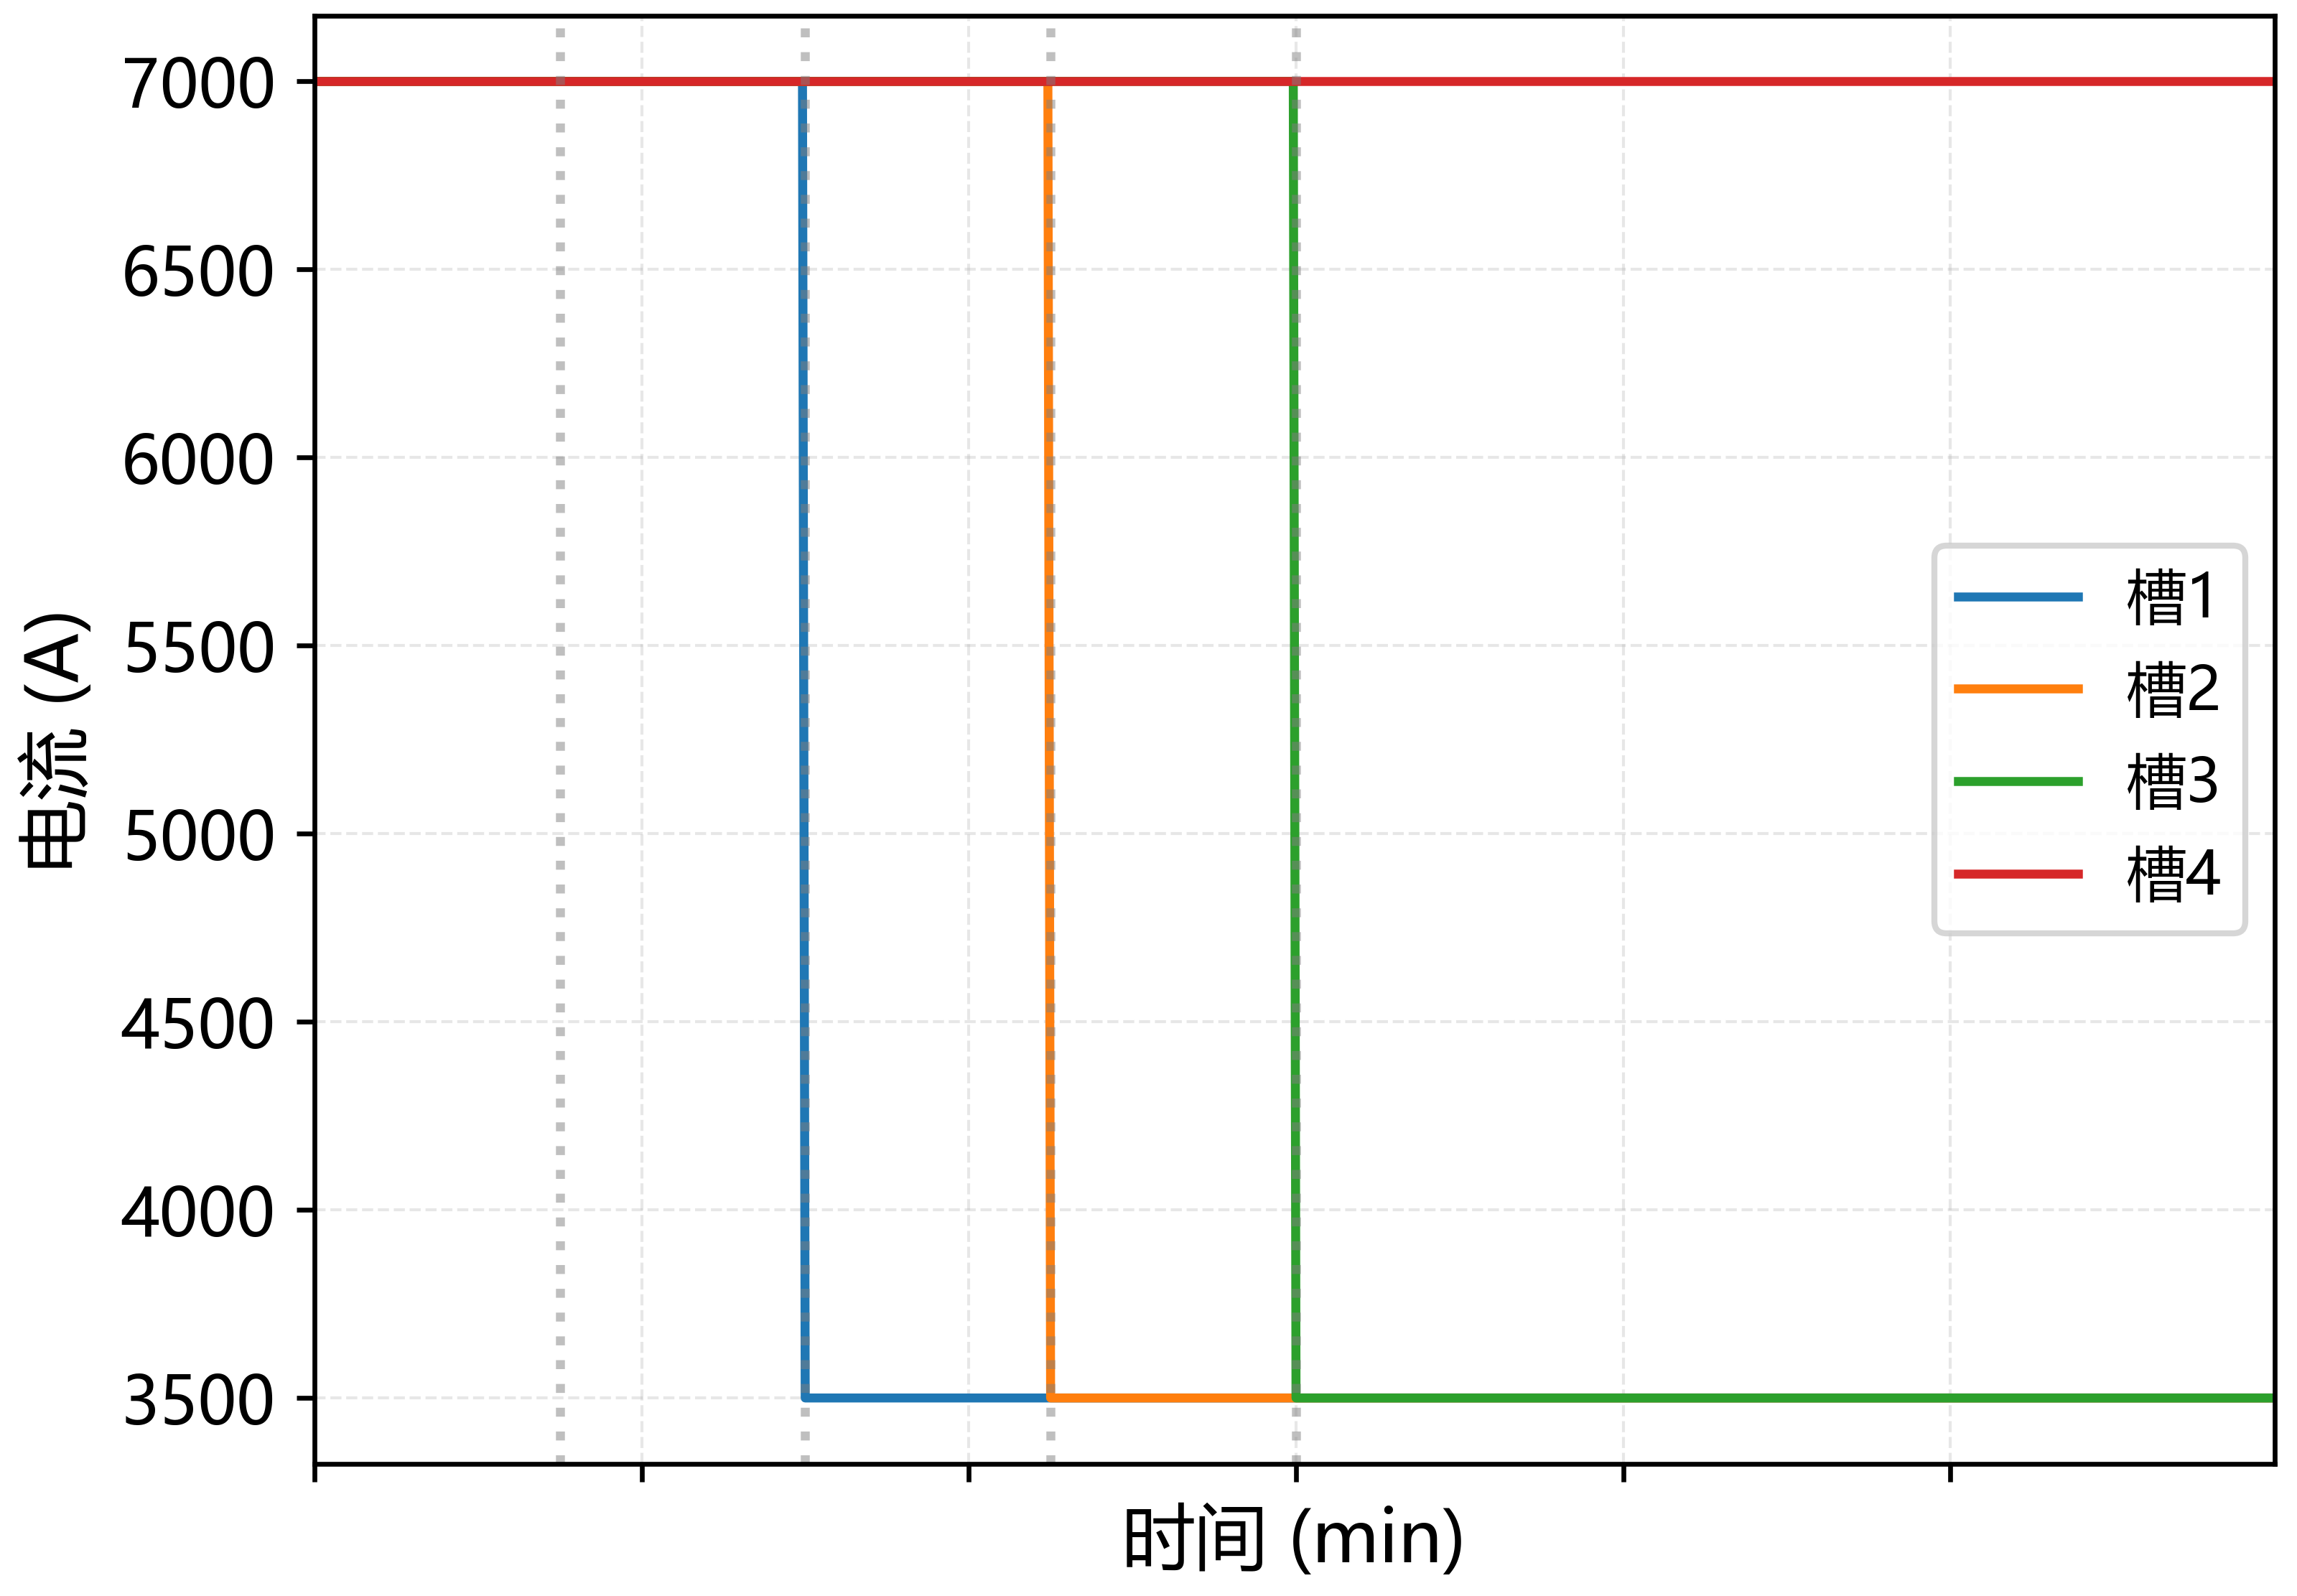
\includegraphics[width=\linewidth]{figures/open_loop_response_a.png}
    \caption{}
  \end{subfigure}
  \hfill
  \begin{subfigure}{0.31\textwidth}
    \centering
    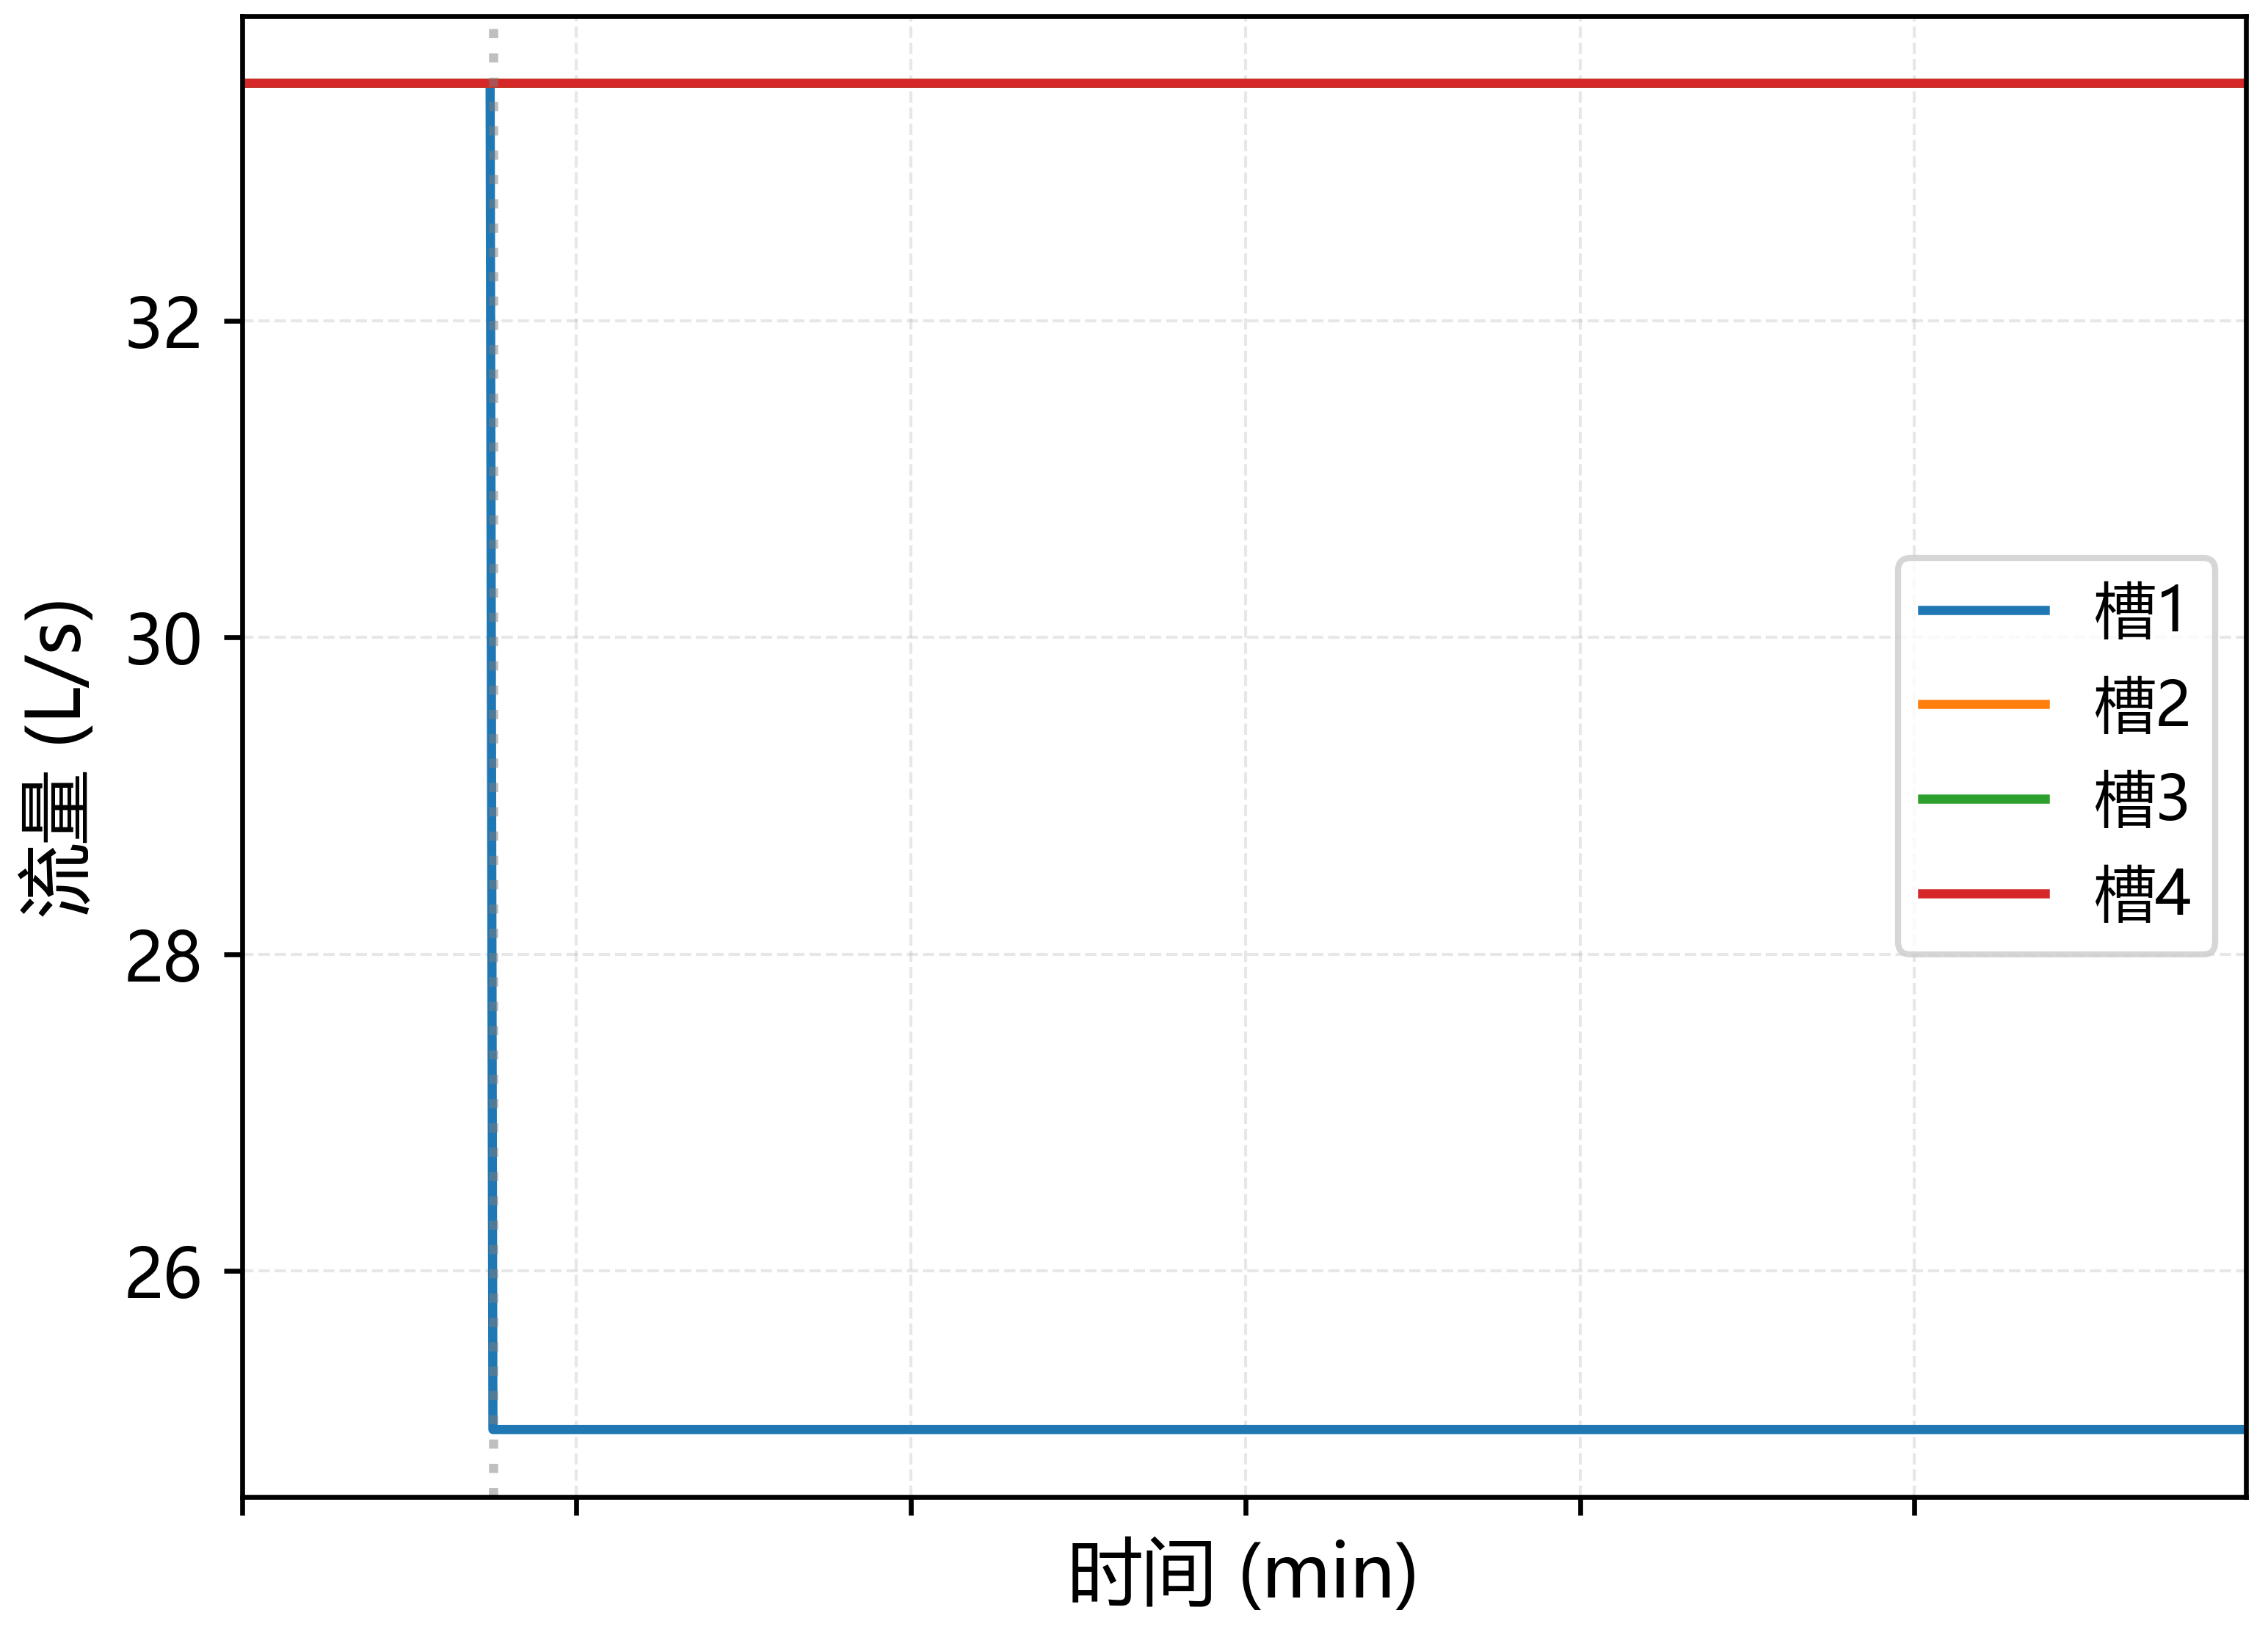
\includegraphics[width=\linewidth]{figures/open_loop_response_b.png}
    \caption{}
  \end{subfigure}
  \hfill
  \begin{subfigure}{0.31\textwidth}
    \centering
    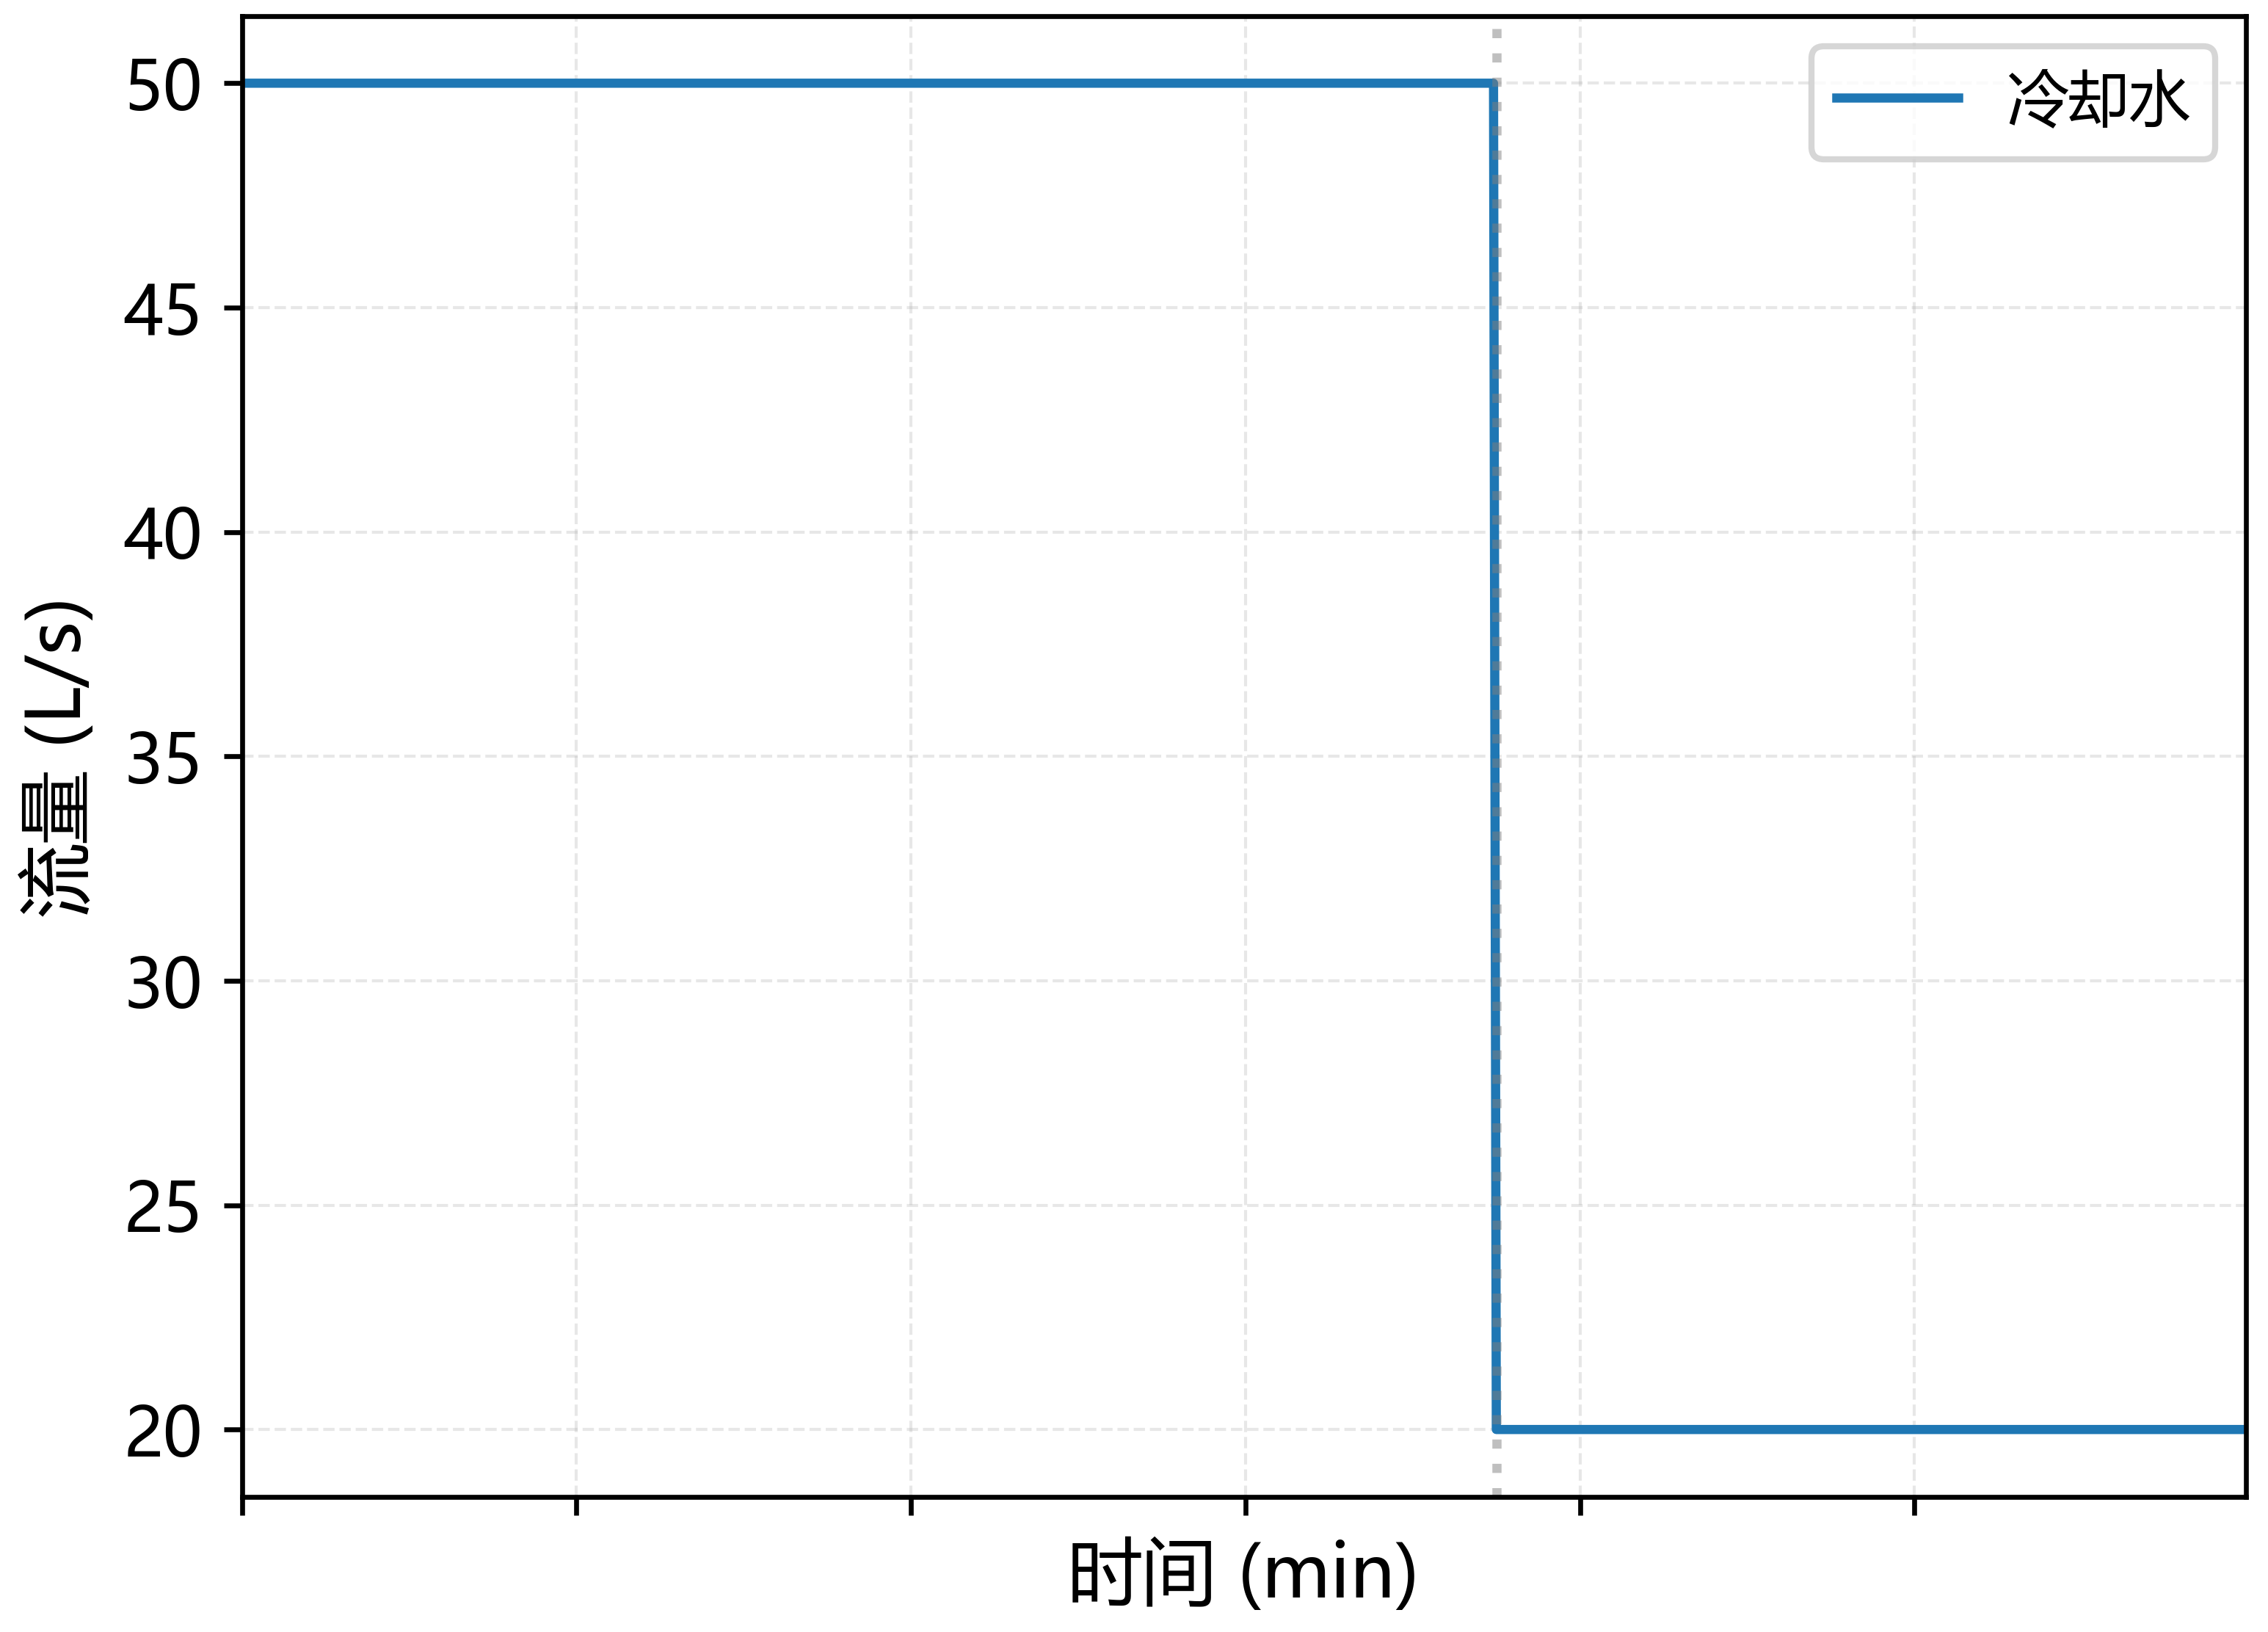
\includegraphics[width=\linewidth]{figures/open_loop_response_c.png}
    \caption{}
  \end{subfigure}

  \vspace{6bp}
  \begin{subfigure}{0.31\textwidth}
    \centering
    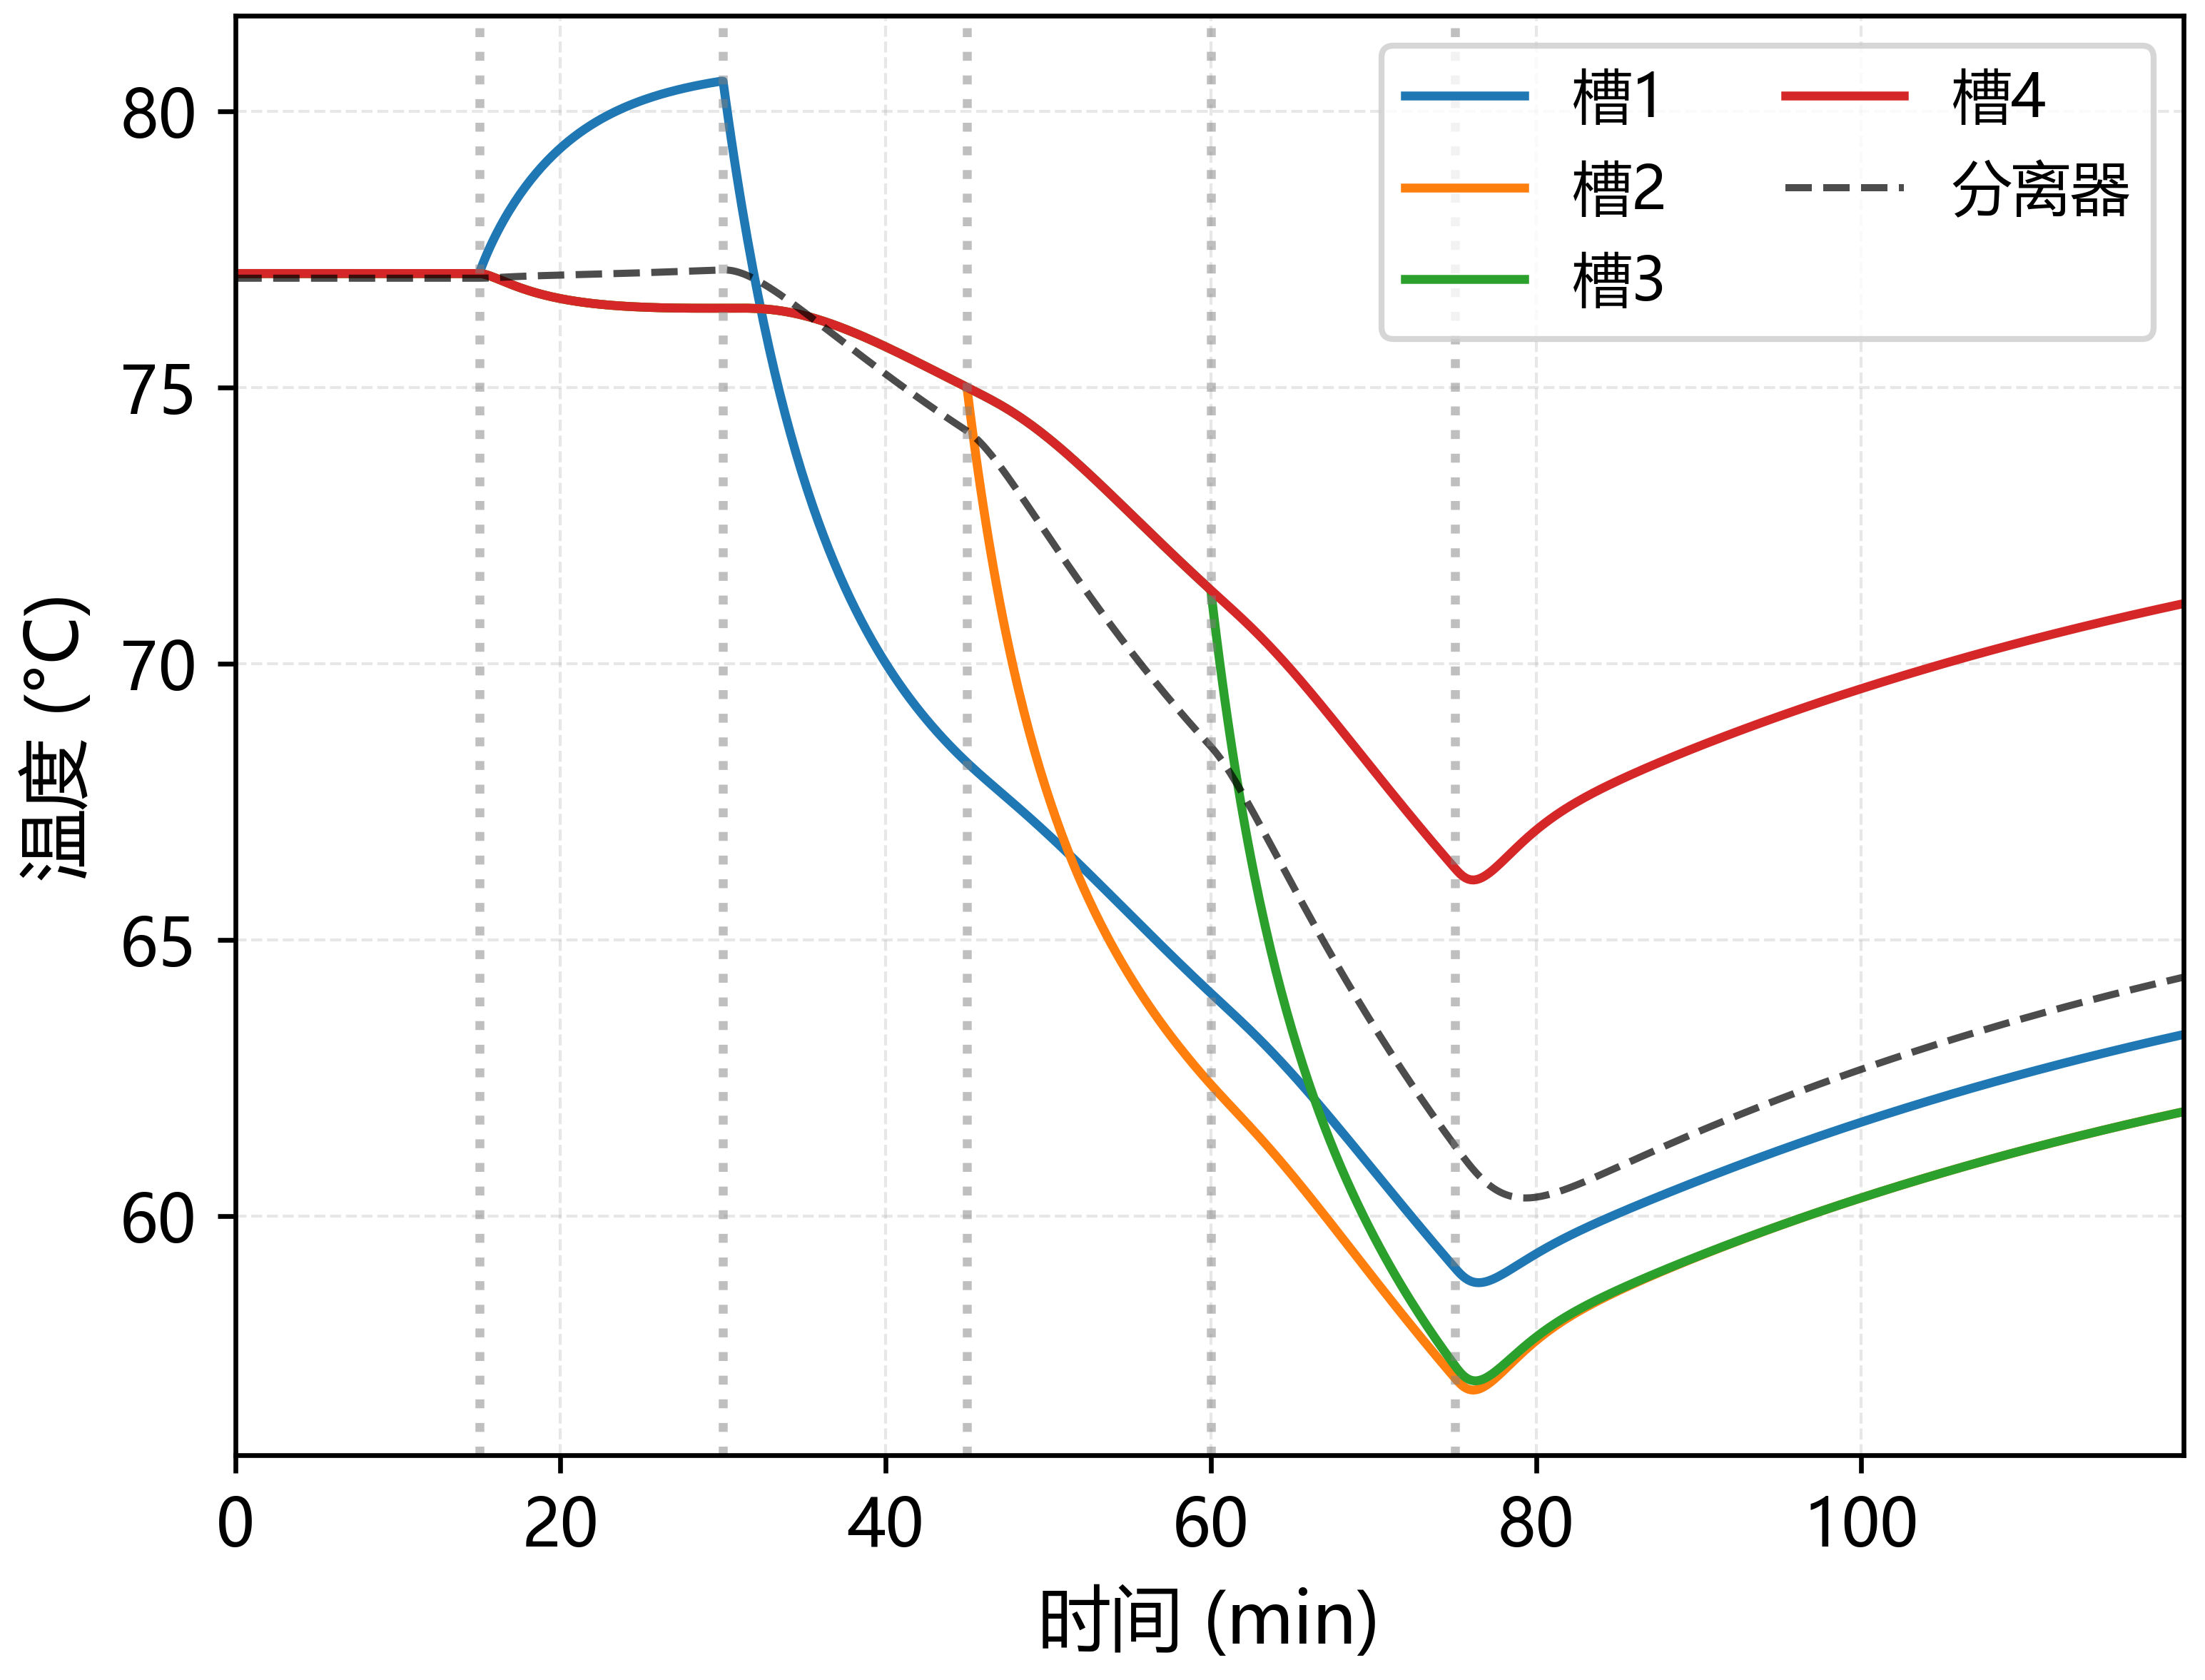
\includegraphics[width=\linewidth]{figures/open_loop_response_d.png}
    \caption{}
  \end{subfigure}
  \hfill
  \begin{subfigure}{0.31\textwidth}
    \centering
    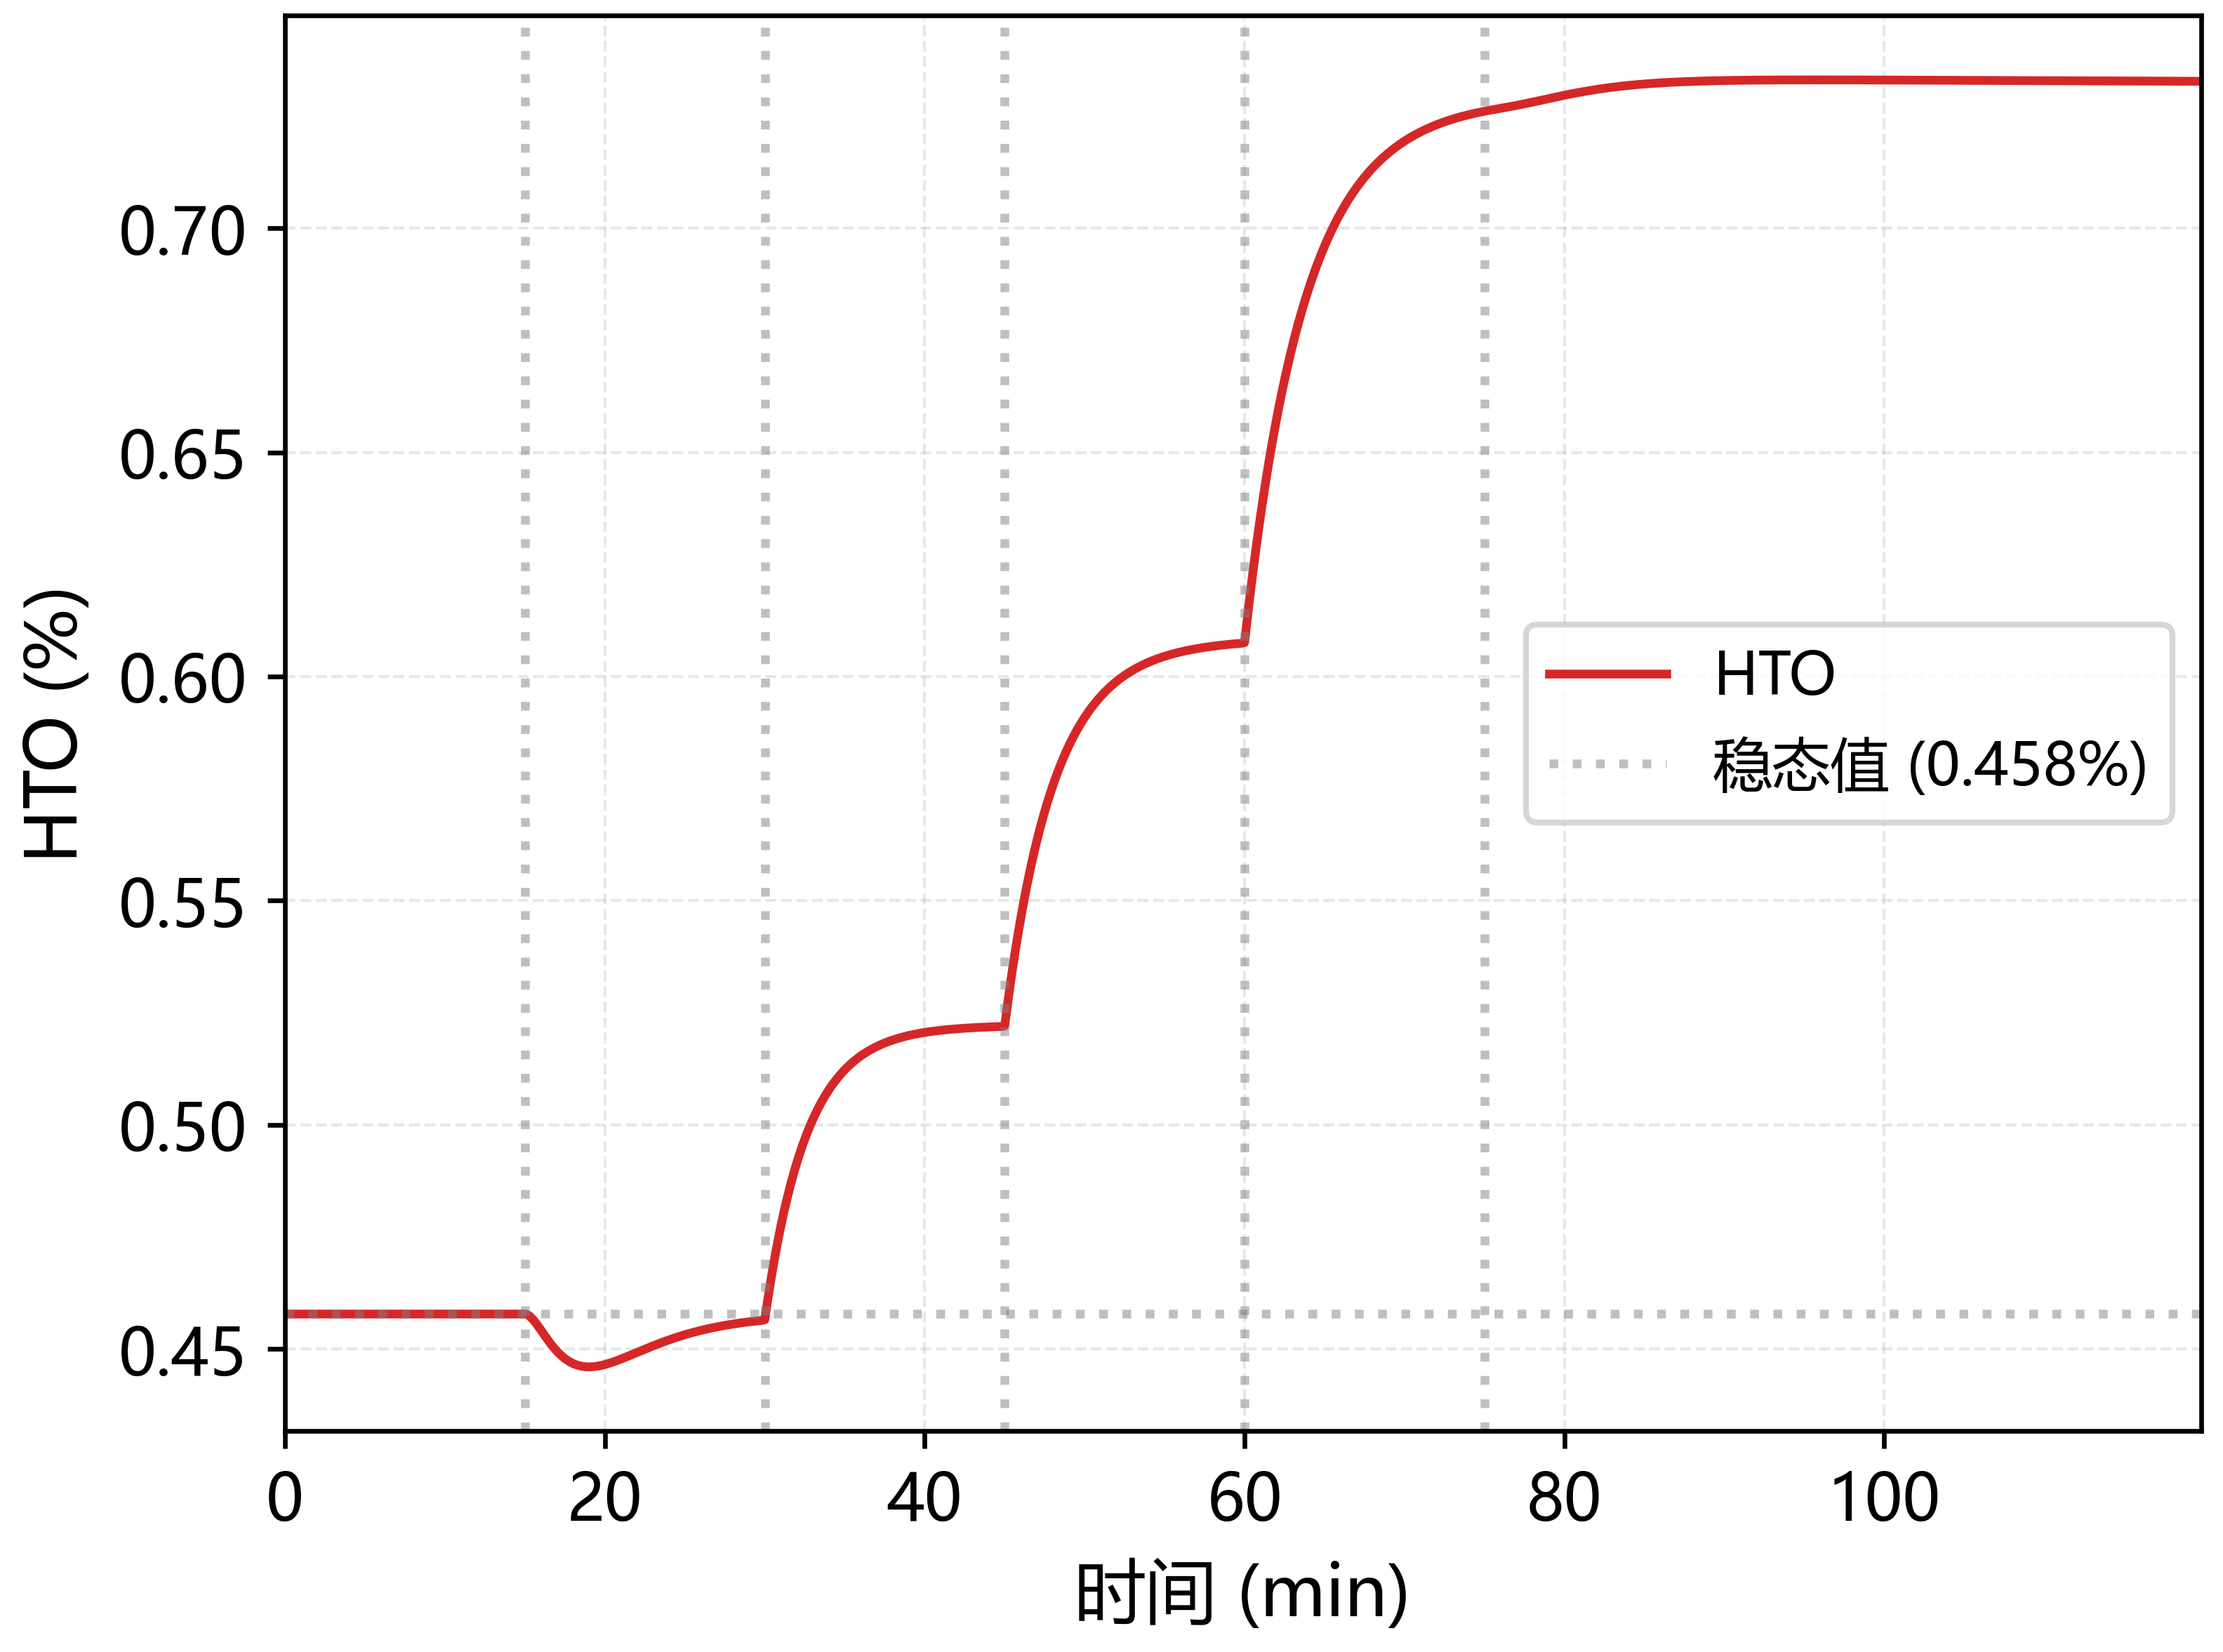
\includegraphics[width=\linewidth]{figures/open_loop_response_e.png}
    \caption{}
  \end{subfigure}
  \hfill
  \begin{subfigure}{0.31\textwidth}
    \centering
    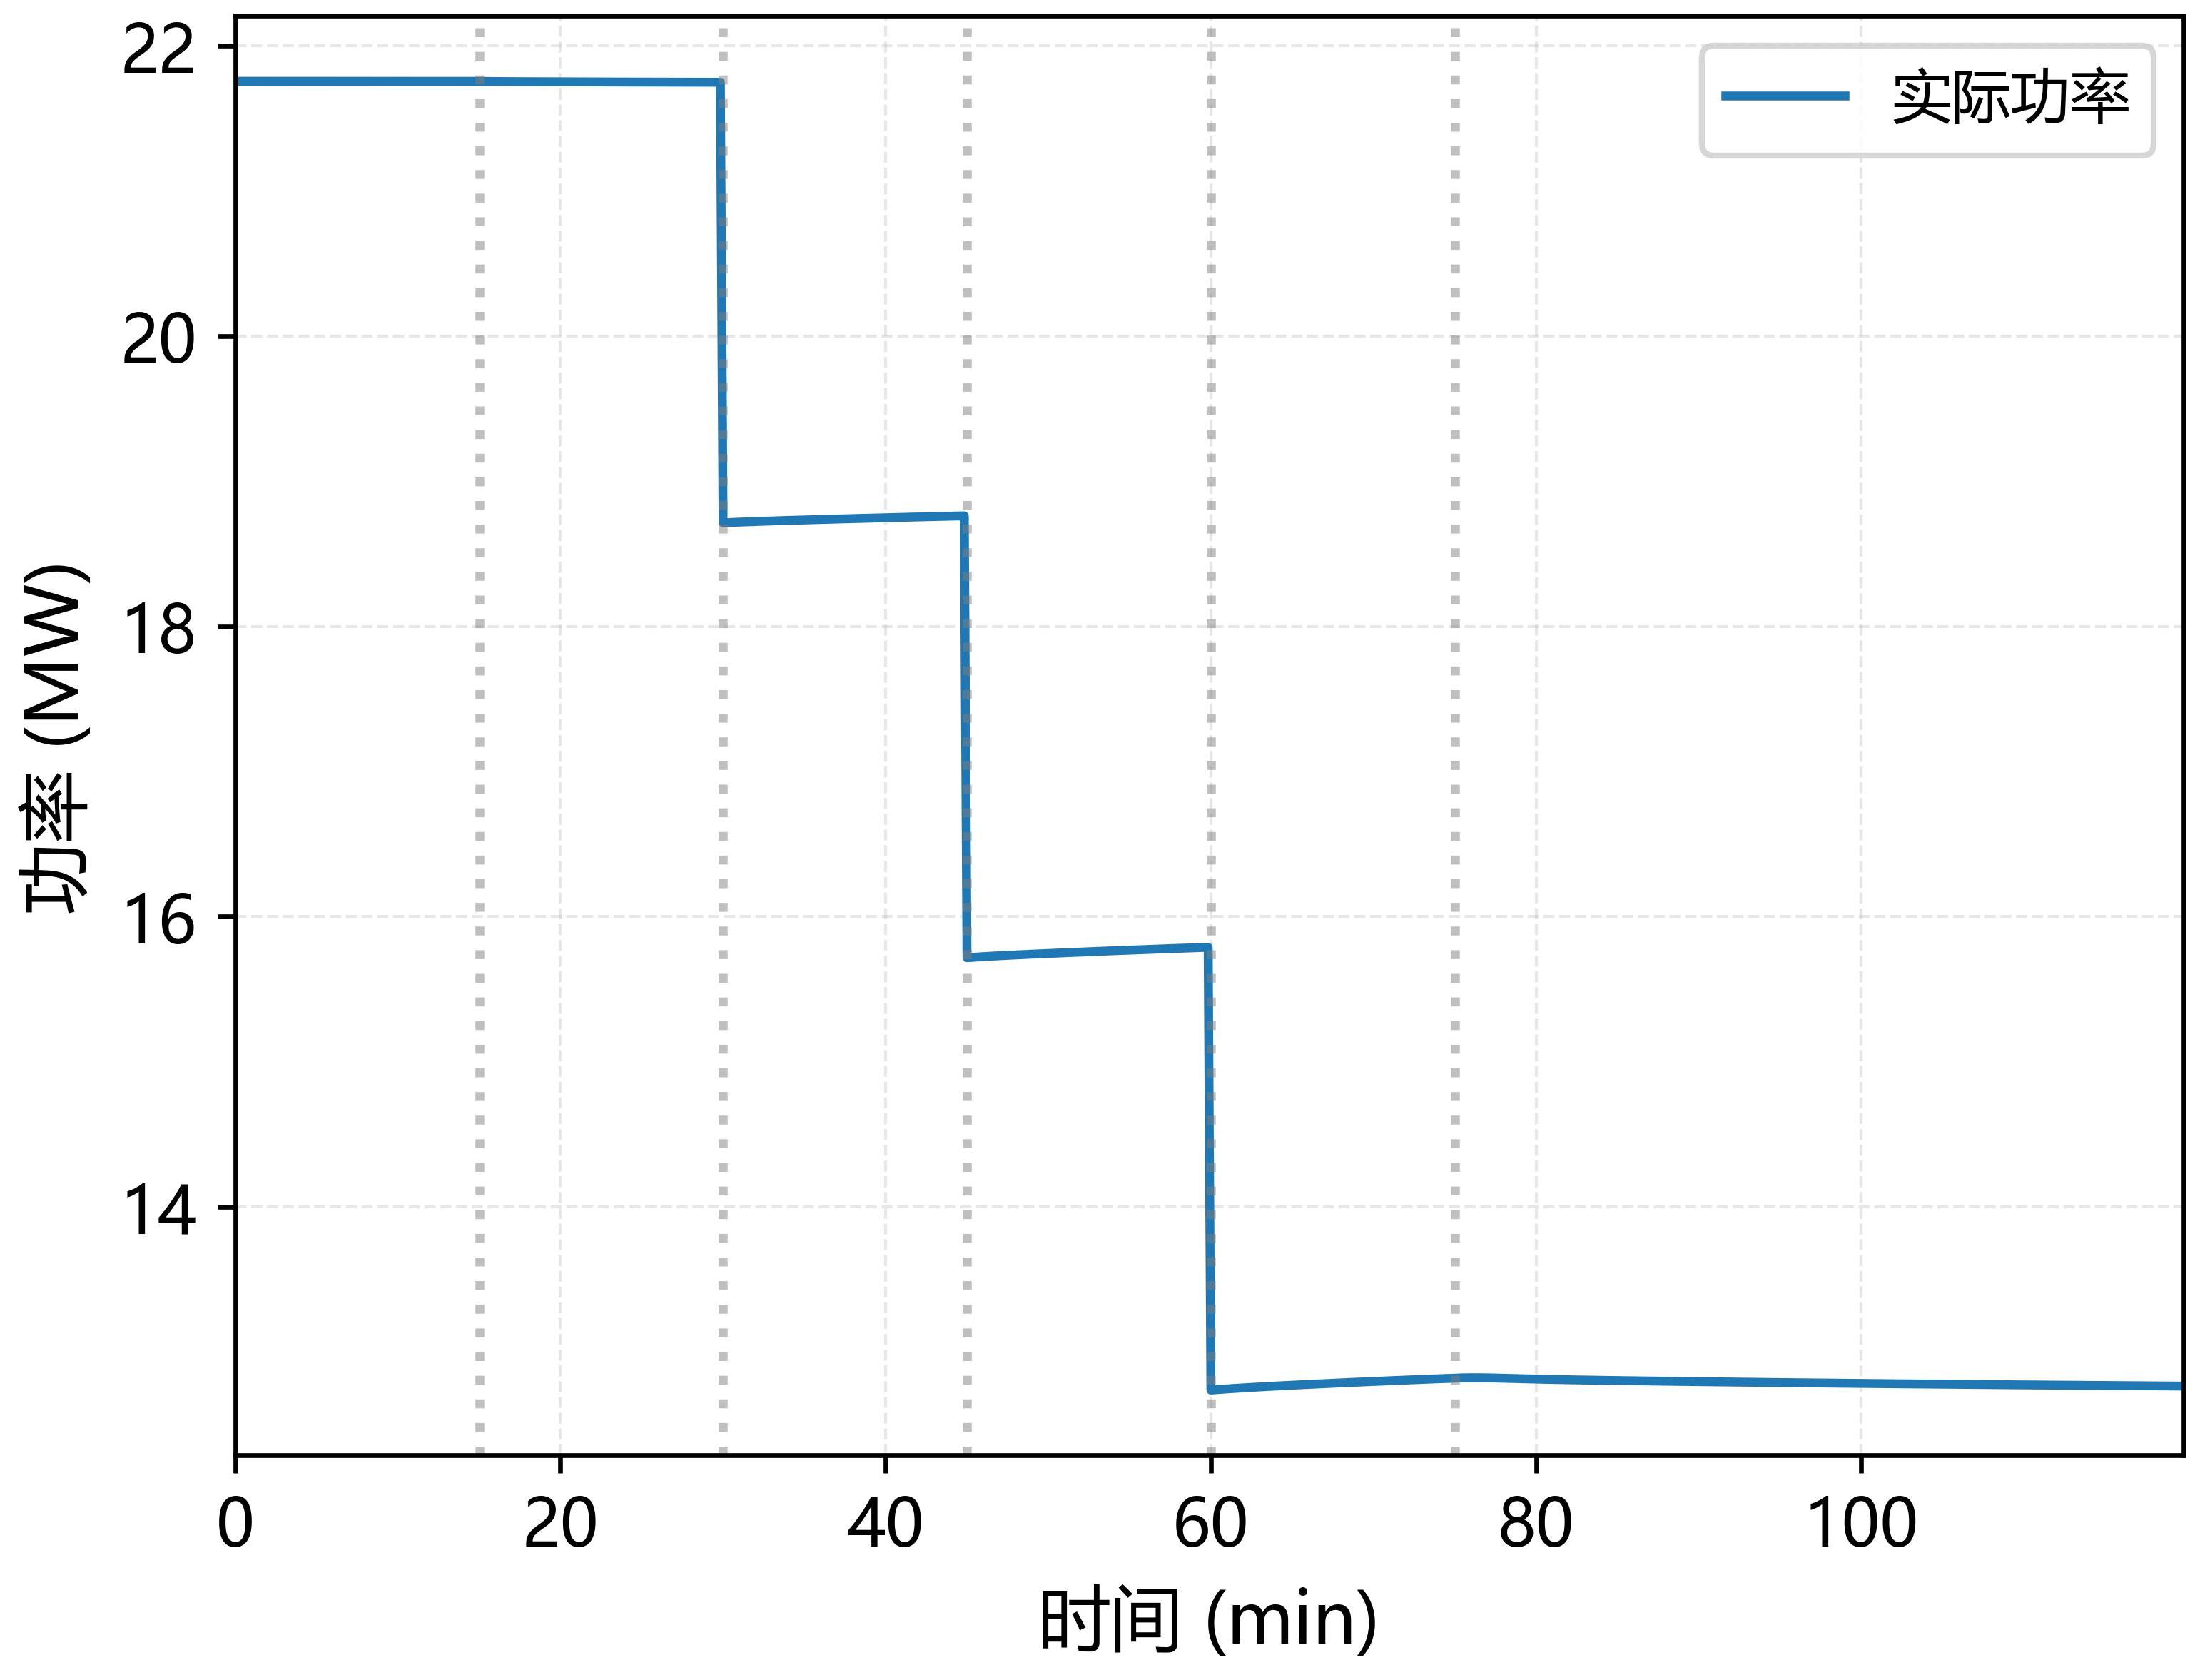
\includegraphics[width=\linewidth]{figures/open_loop_response_f.png}
    \caption{}
  \end{subfigure}
  \caption{多槽AWE系统开环动态响应}
  \captionsetup{font=normalfont}
  \caption*{(a) 电解槽电流；(b) 碱液流量；(c) 冷却水流量；(d) 电解槽与分离器温度；(e) HTO浓度；(f) 总功率}
  \label{fig:open_loop_response}
\end{figure}

\subsection{闭环实验}

\subsubsection{阶跃响应实验}

为验证TCN Diffusion控制器在功率突变工况下的动态响应特性，设计了10~MW至20~MW阶跃响应实验。
实验设置如下：前120~min系统运行于10~MW稳态功率，在$t=120$~min时刻功率参考值阶跃跃升至20~MW，总仿真时长240~min。
对比对象包括TCN Diffusion、Diffusion MLP、NMPC与MLP四种方法，评价指标涵盖功率跟踪精度（RMSE、MAE、上升时间与超调量）、温度控制品质（MAE与最大偏差）、HTO安全性以及控制量平滑性（碱液流量与冷却水流量的波动范围）。

图~\ref{fig:controller_step_comparison} 展示了四种方法在该阶跃工况下的闭环响应。
功率跟踪方面，各方法动态响应差异明显。NMPC基于在线优化求解，上升最快（约28.2~min）且无超调；扩散模型策略的上升时间介于31--34~min，超调控制在0.5\%以内，其中TCN Diffusion因时序卷积结构对功率突变具有更强的惯性缓冲，上升最为平缓；纯MLP的上升时间达47.0~min且存在约5.6\%的欠调，反映出其纯前馈结构对功率阶跃瞬态的预测能力不足。从跟踪误差来看，功率RMSE由低到高依次为NMPC（2.30~MW）、TCN Diffusion（2.43~MW）、Diffusion MLP（2.58~MW）与MLP（2.64~MW），时序建模能力的缺失导致MLP的预测滞后最为显著。
温度控制方面，TCN Diffusion表现最优，温度MAE仅为0.286~K，最大偏差0.54~K；NMPC次之，MAE为0.329~K；MLP作为无扩散过程的纯神经网络基线，温度MAE达1.42~K，最大偏差约4.85~K，温度波动范围为77.5--86.2$^\circ$C，反映纯MLP网络对热动态长期依赖的时序建模能力严重不足；Diffusion MLP的温度偏差亦显著较大，MAE为0.978~K，最大偏差1.47~K，温度波动范围为78.53--80.27$^\circ$C，说明扩散去噪过程虽能在一定程度上提升温度预测鲁棒性，但仍难以弥补MLP主干网络在时序建模上的本质缺陷。
HTO安全方面，四种方法均能将气相氢气浓度控制在2\%安全阈值以下，峰值均在0.88--1.17\%左右。
控制量调节特性与动态建模能力密切相关。四种方法的总电流变化范围基本一致（约8--26~kA），因为电流直接决定功率输出，各控制器均优先保证功率跟踪精度；但碱液流量的调节行为呈现显著分化：MLP因缺乏时序记忆，难以预判气液分离过程的动态惯性，流量调节呈现剧烈振荡（波动范围38.5--51.2~L/s）；Diffusion MLP虽引入扩散去噪，但MLP主干网络仍难以捕捉碱液循环的长期依赖（40.3--46.8~L/s）；TCN Diffusion凭借时序卷积结构对历史状态的有效聚合，流量变化最为平缓（26.5--36.1~L/s），已接近NMPC的在线优化水平（19.5--28.2~L/s）。这表明时序建模能力直接决定了多变量协调控制的平滑性。

\begin{figure}[!htbp]
  \centering
  \begin{subfigure}{0.48\textwidth}
    \centering
    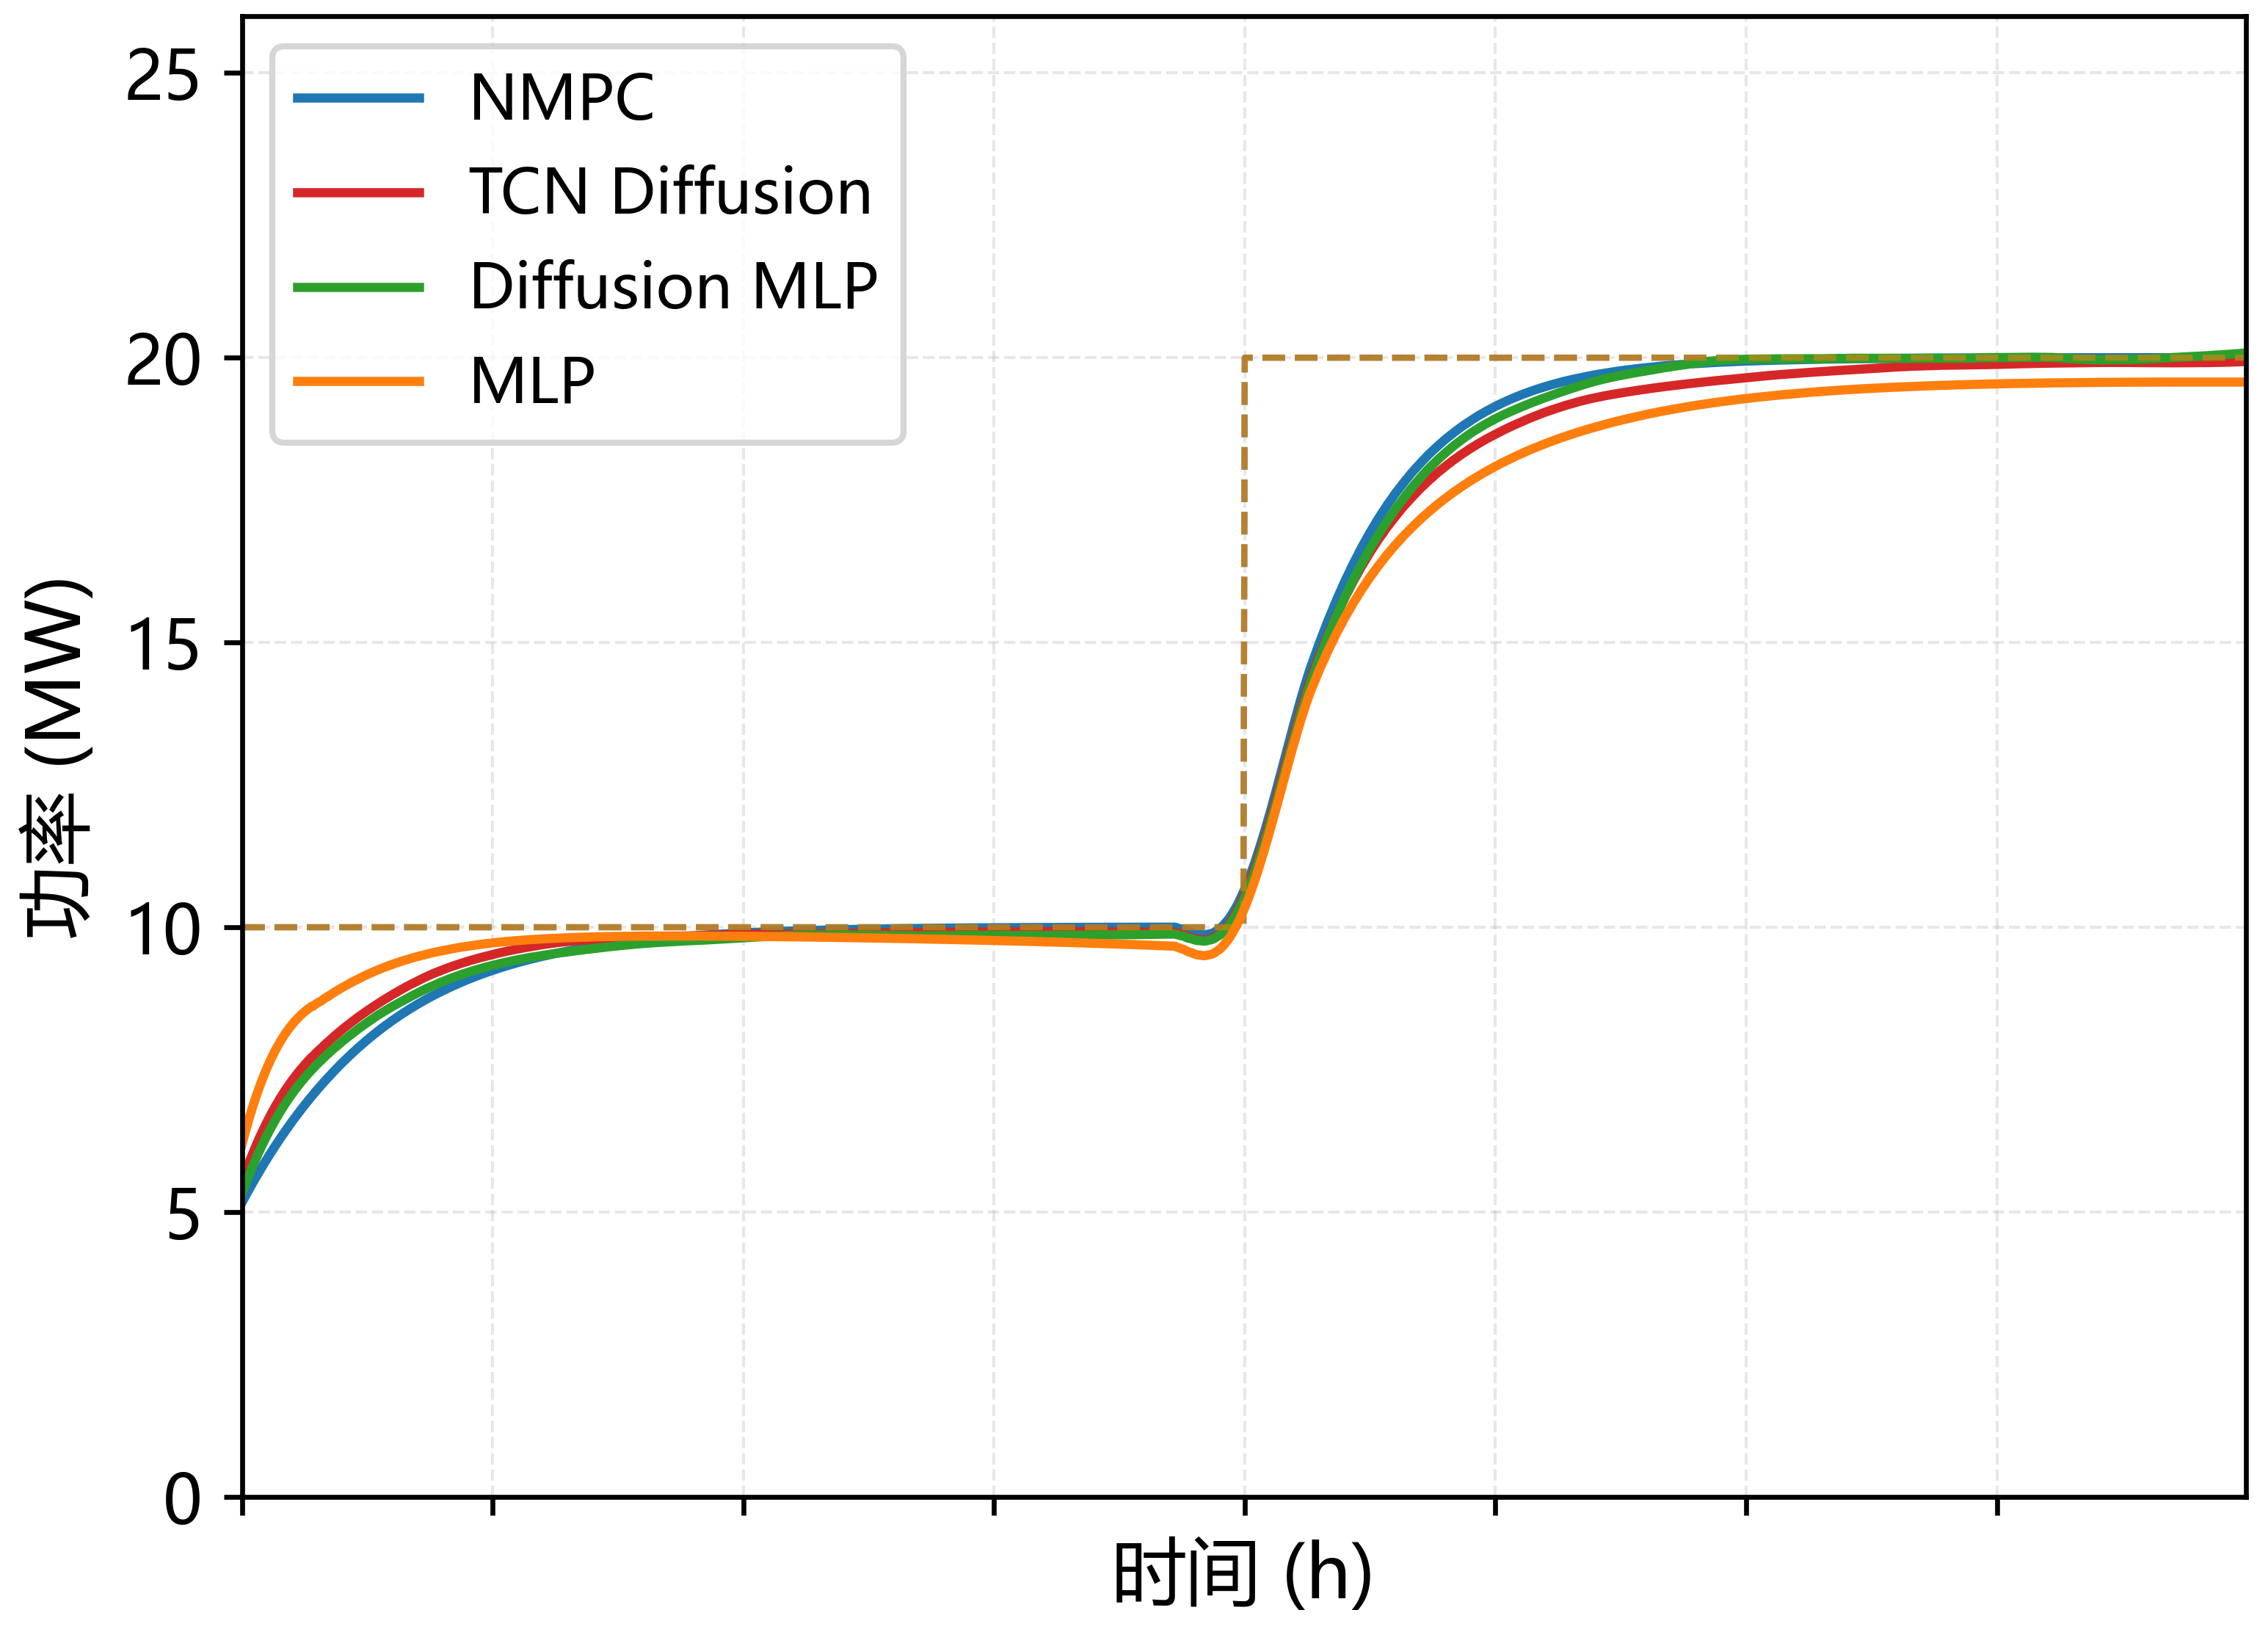
\includegraphics[width=\linewidth]{figures/controller_step_comparison_a.png}
    \caption{}
  \end{subfigure}
  \hfill
  \begin{subfigure}{0.48\textwidth}
    \centering
    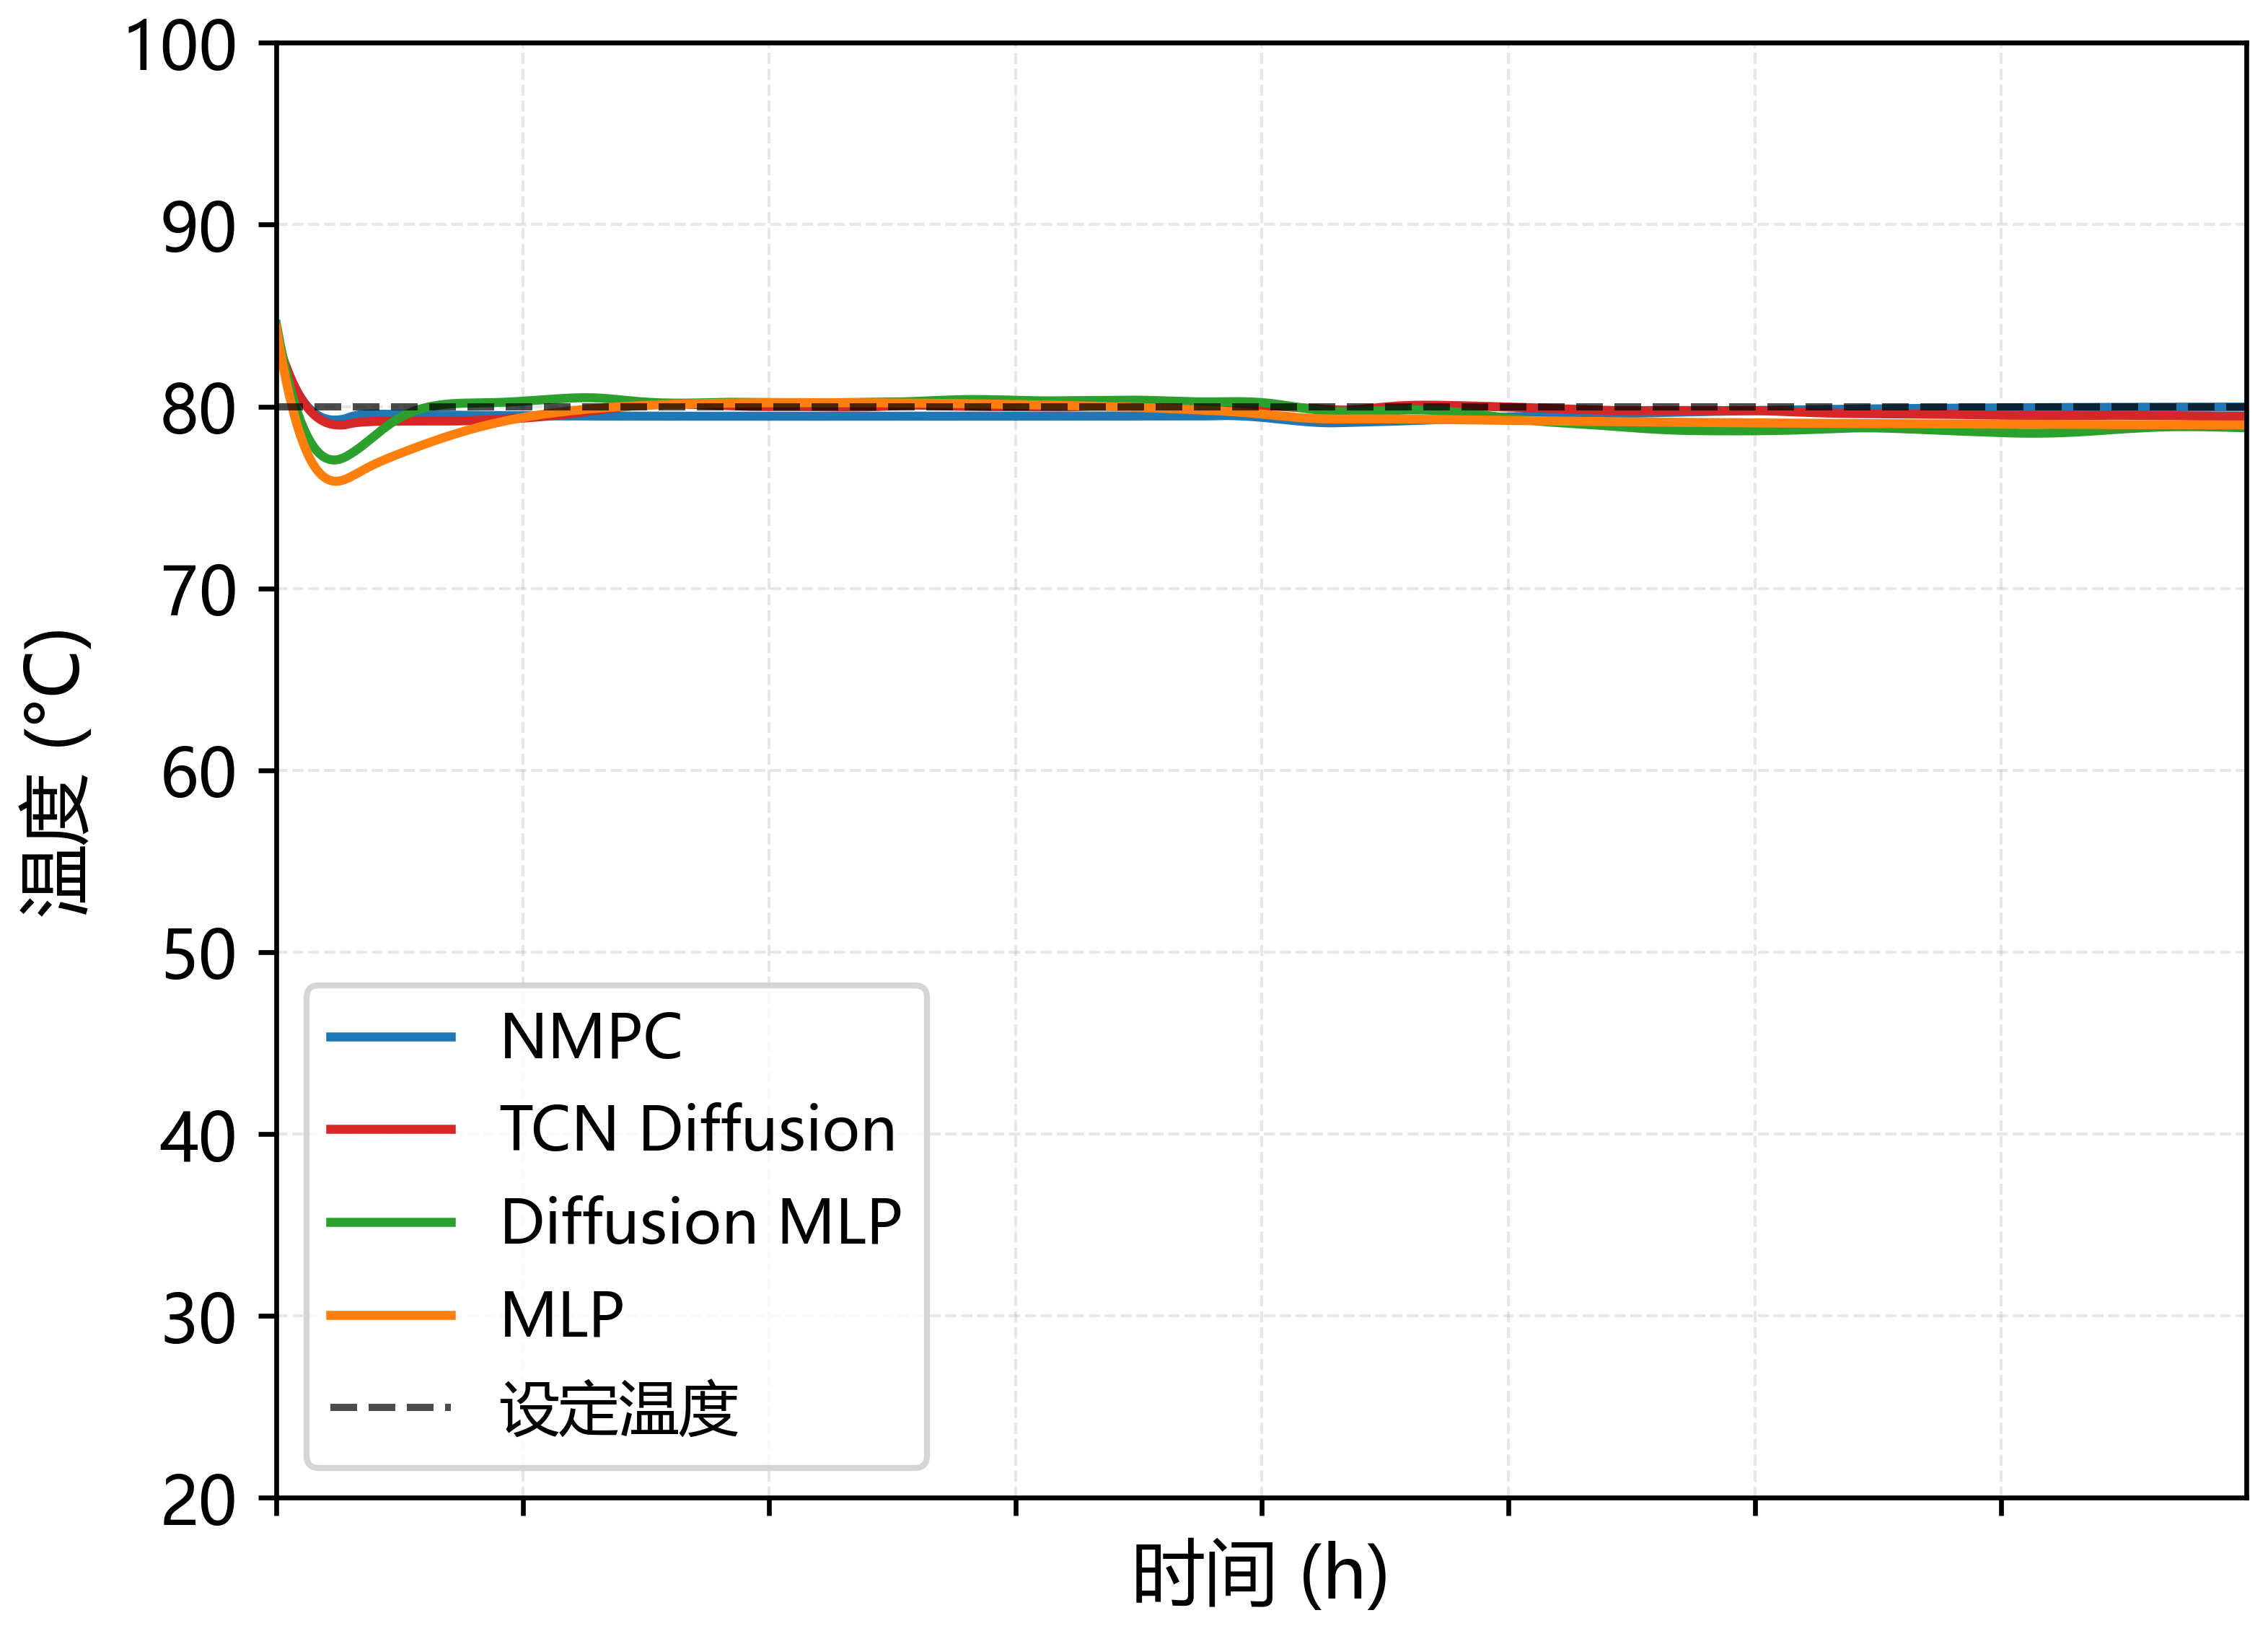
\includegraphics[width=\linewidth]{figures/controller_step_comparison_b.png}
    \caption{}
  \end{subfigure}

  \begin{subfigure}{0.48\textwidth}
    \centering
    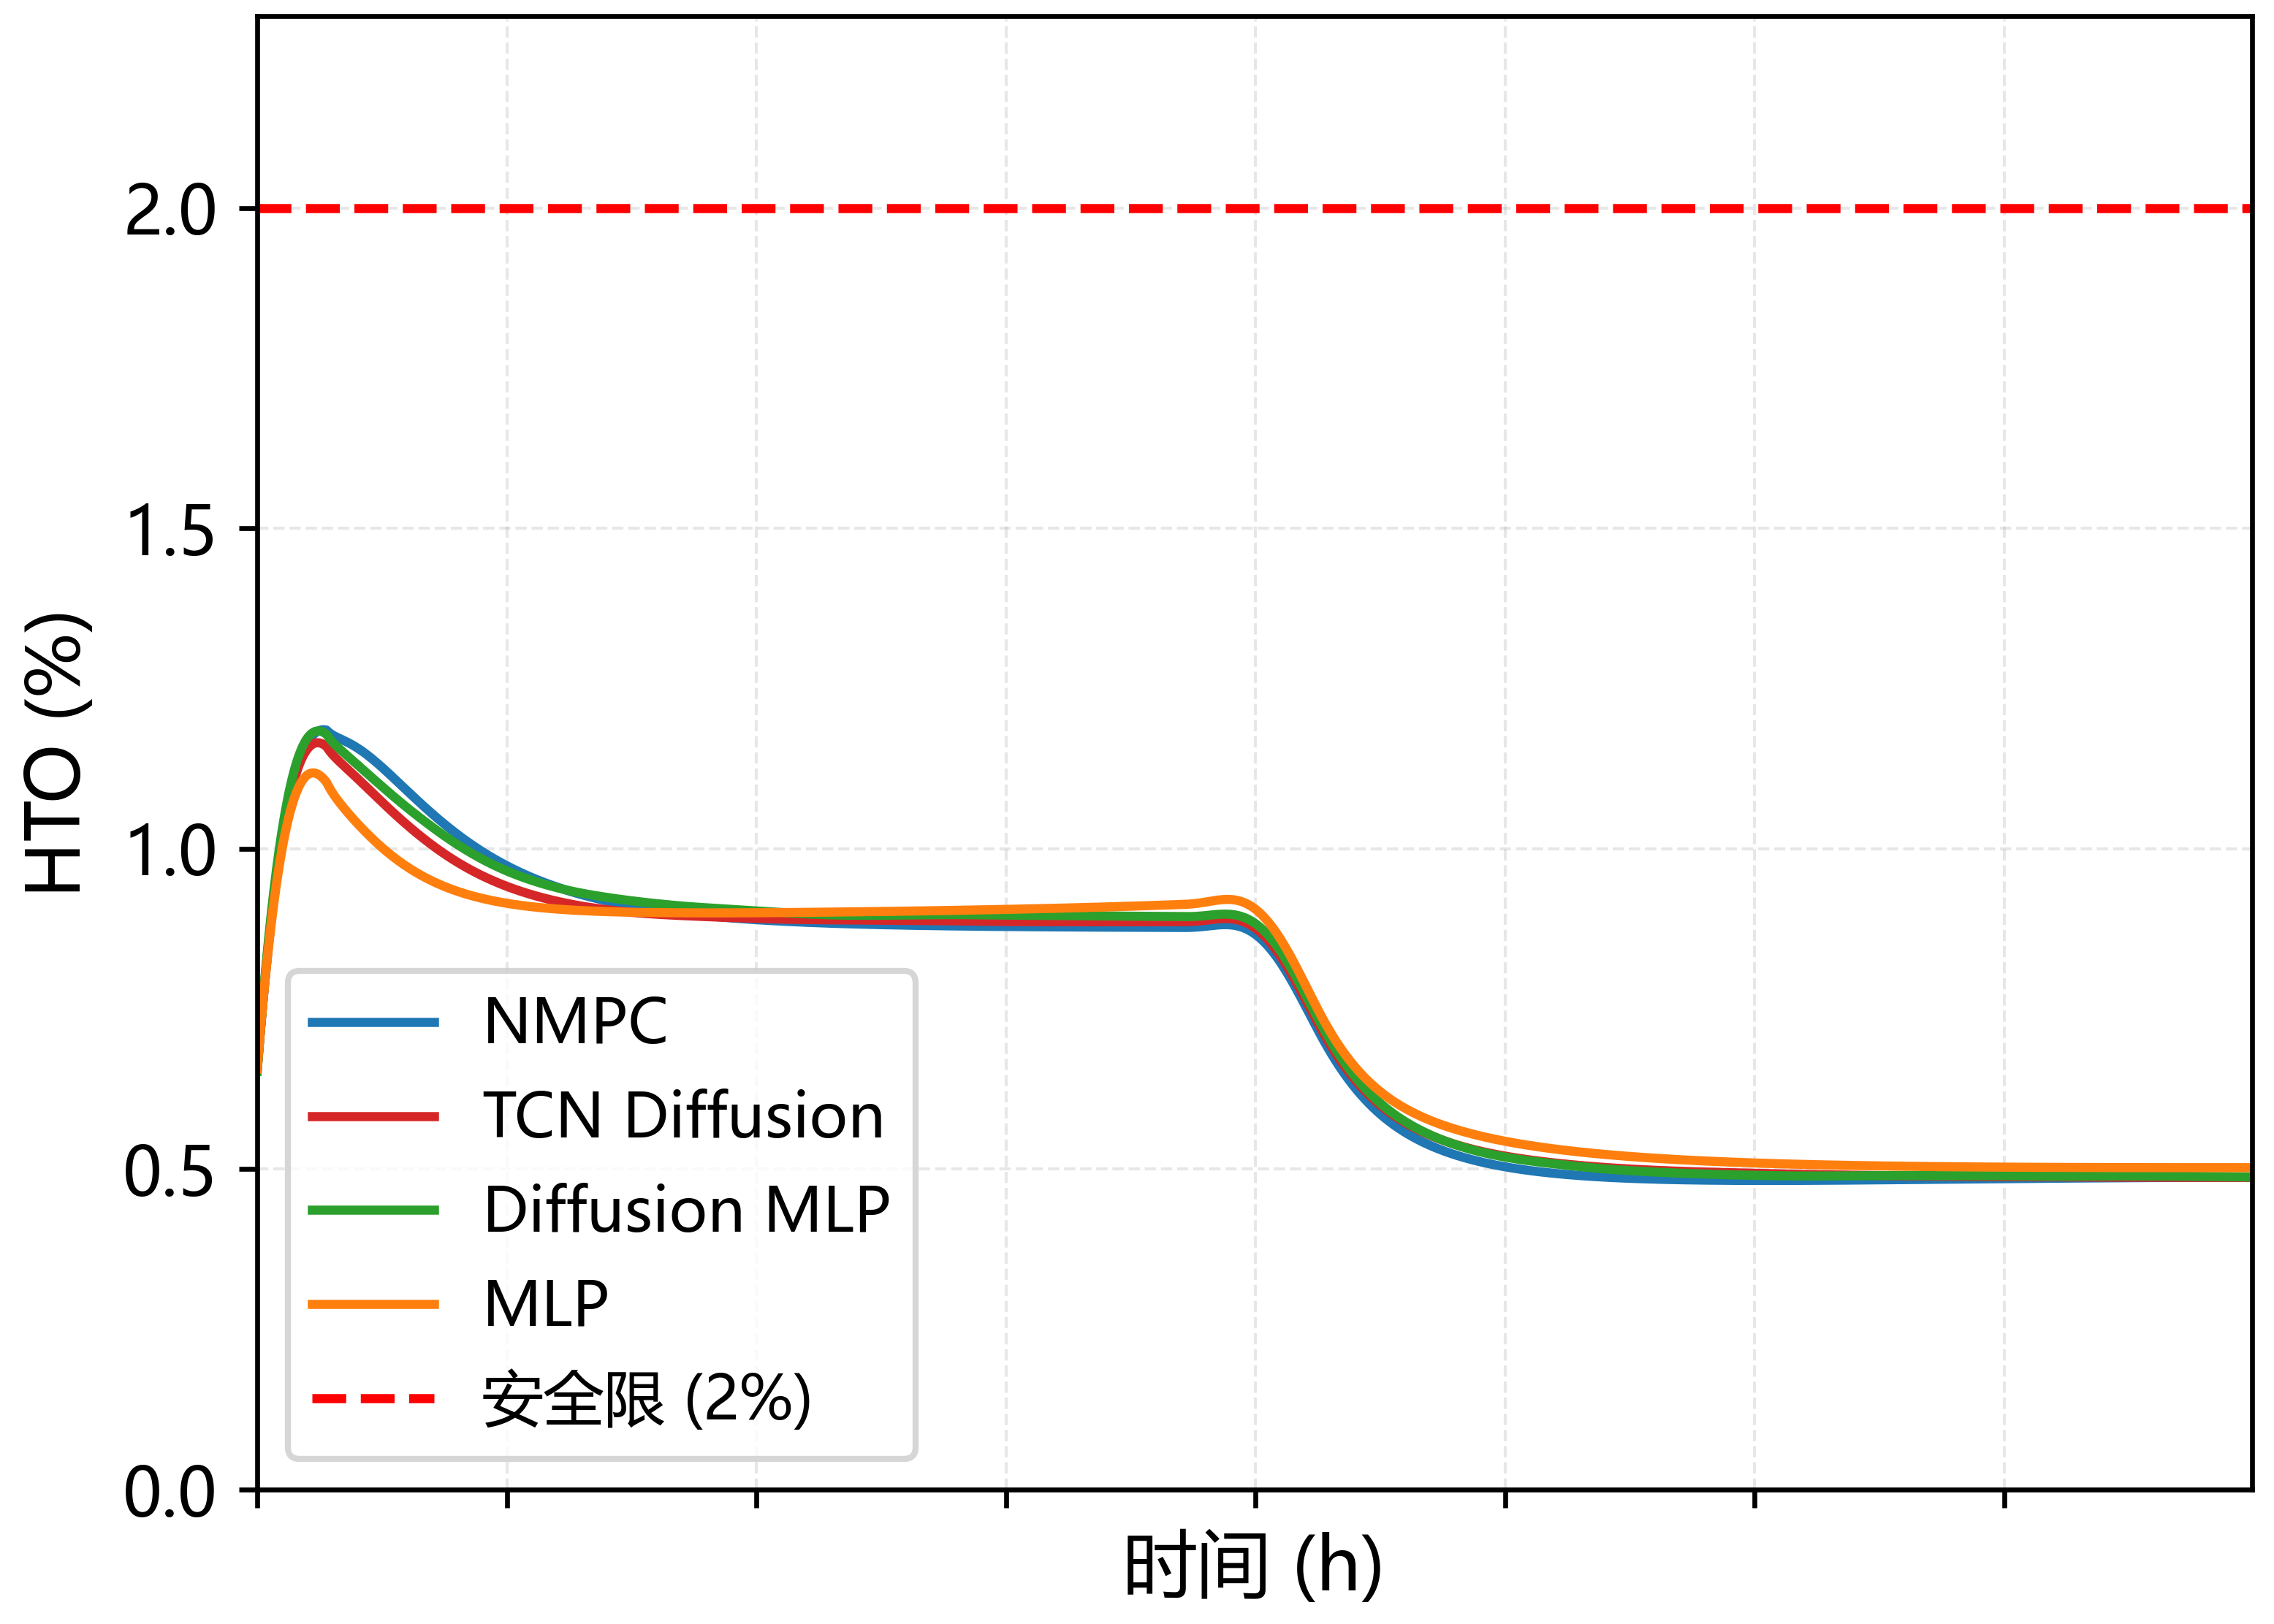
\includegraphics[width=\linewidth]{figures/controller_step_comparison_c.png}
    \caption{}
  \end{subfigure}
  \hfill
  \begin{subfigure}{0.48\textwidth}
    \centering
    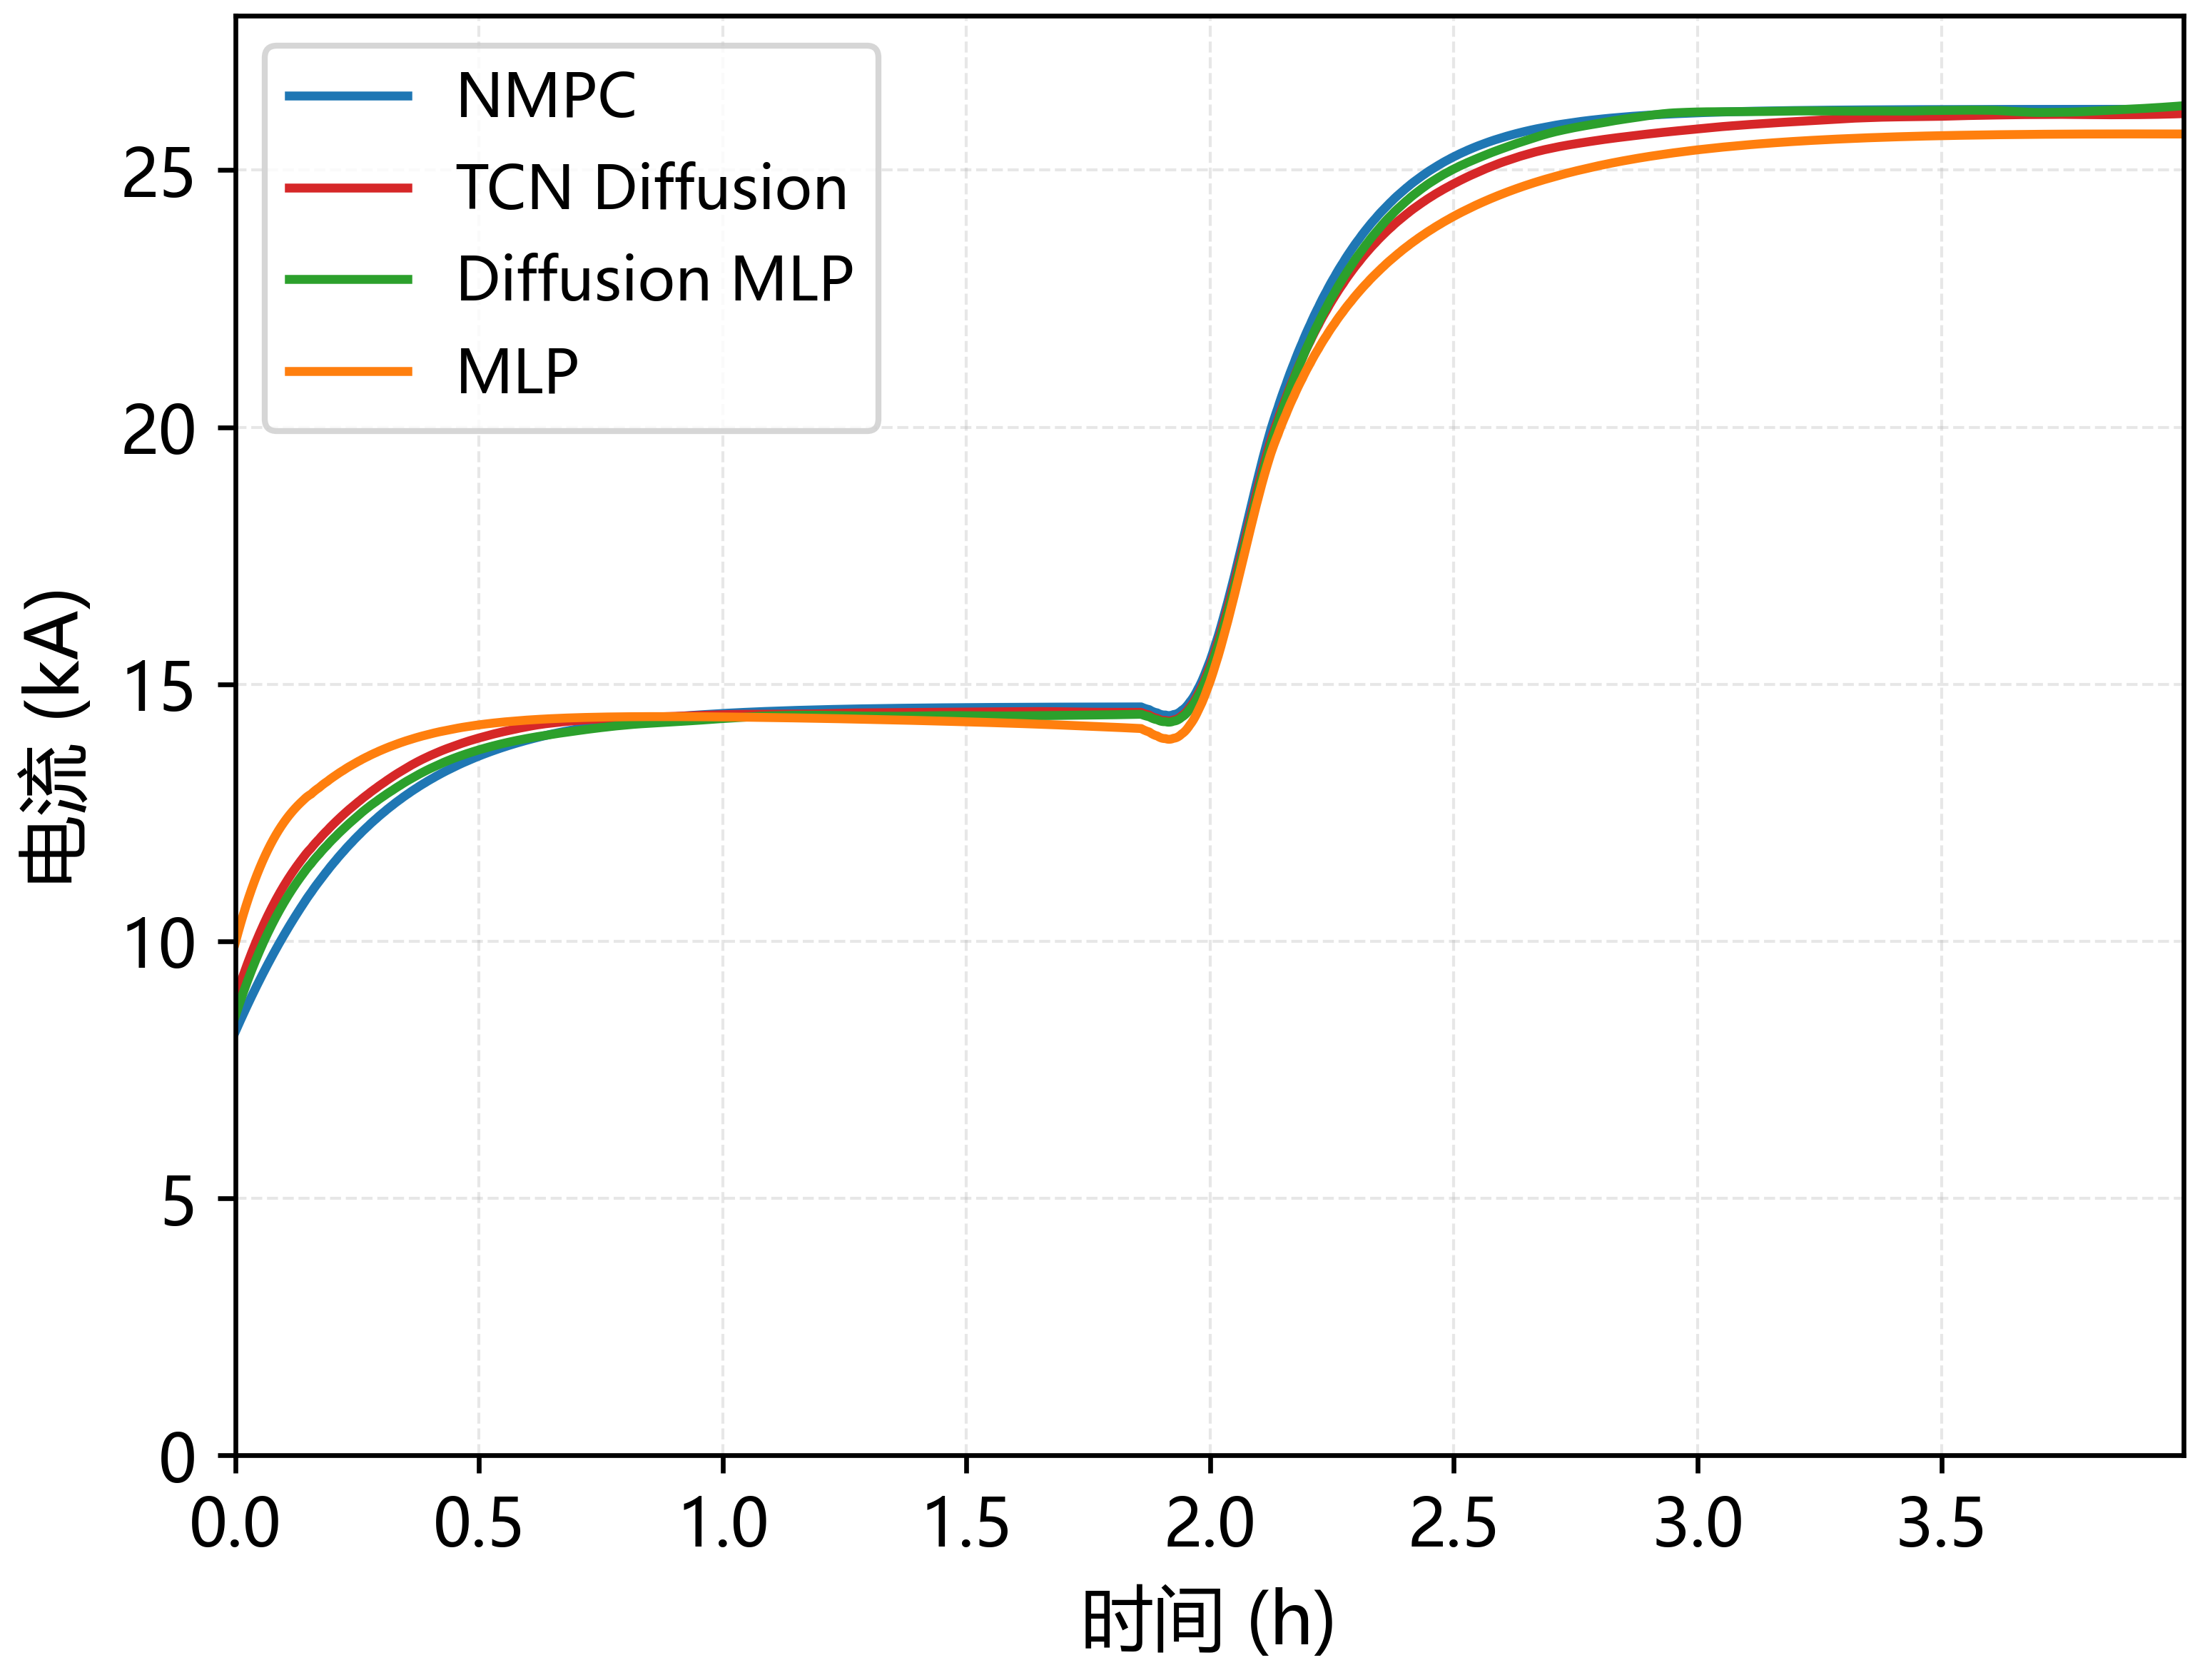
\includegraphics[width=\linewidth]{figures/controller_step_comparison_d.png}
    \caption{}
  \end{subfigure}

  \begin{subfigure}{0.48\textwidth}
    \centering
    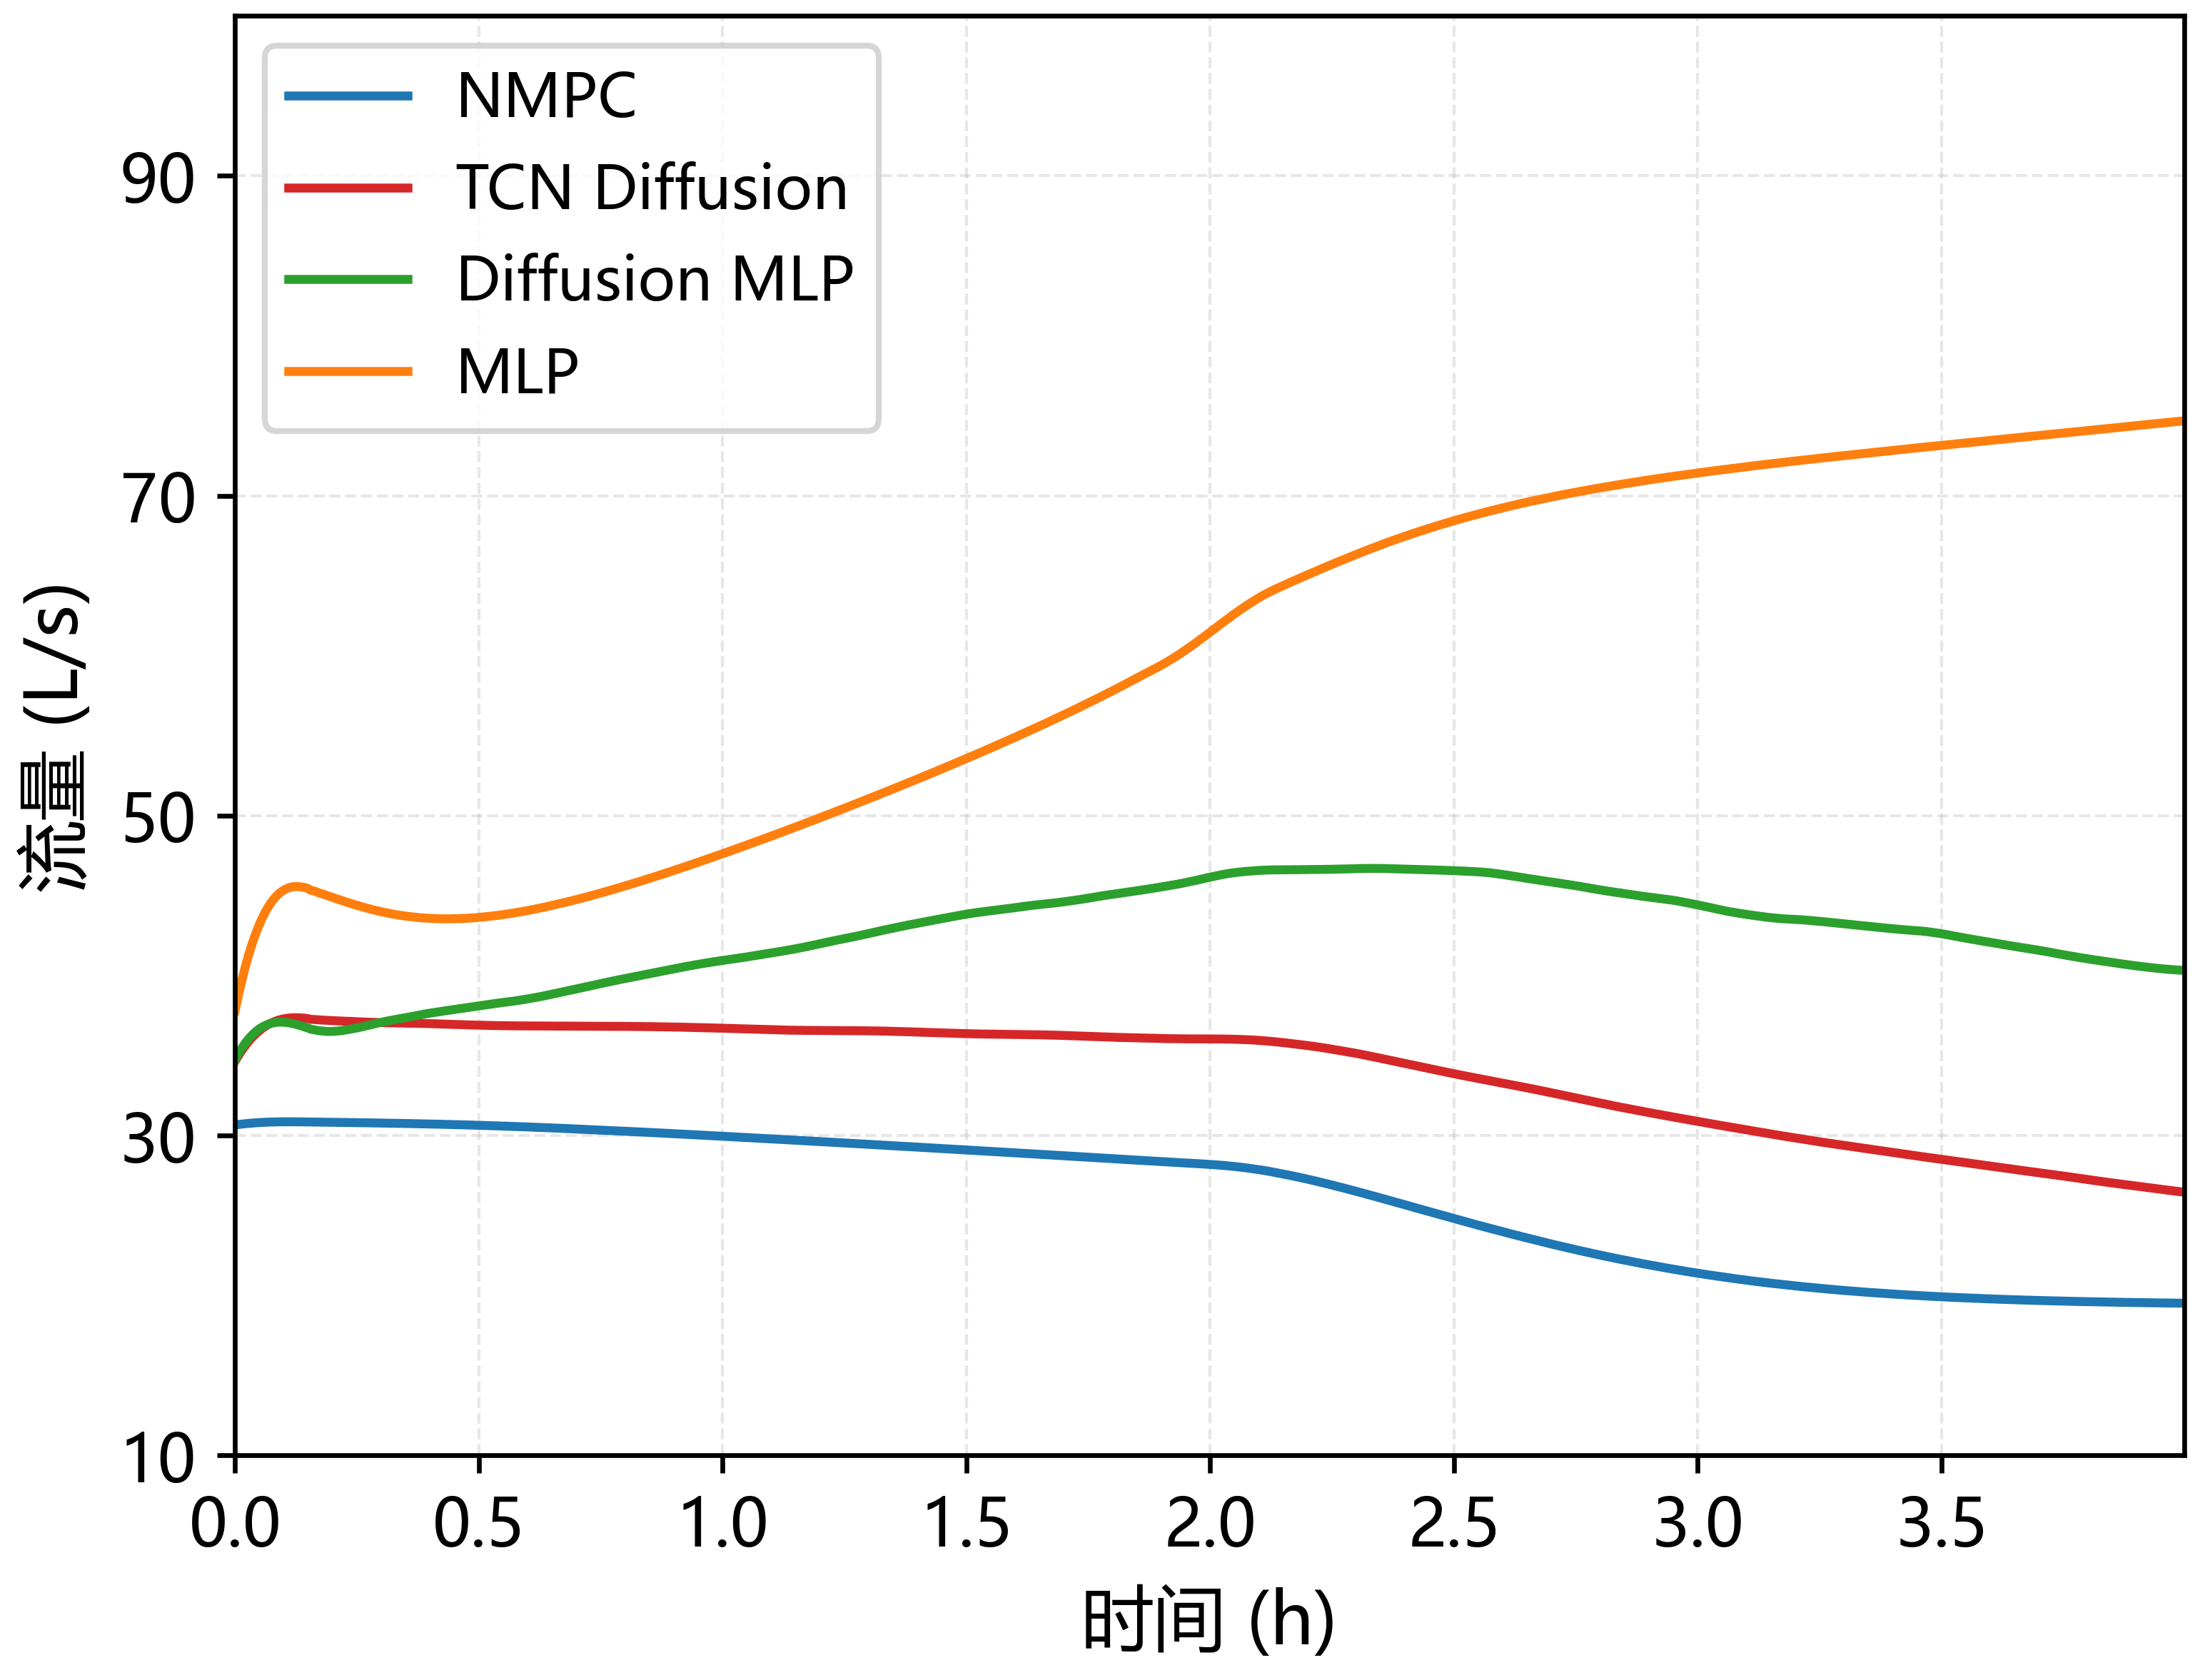
\includegraphics[width=\linewidth]{figures/controller_step_comparison_e.png}
    \caption{}
  \end{subfigure}
  \hfill
  \begin{subfigure}{0.48\textwidth}
    \centering
    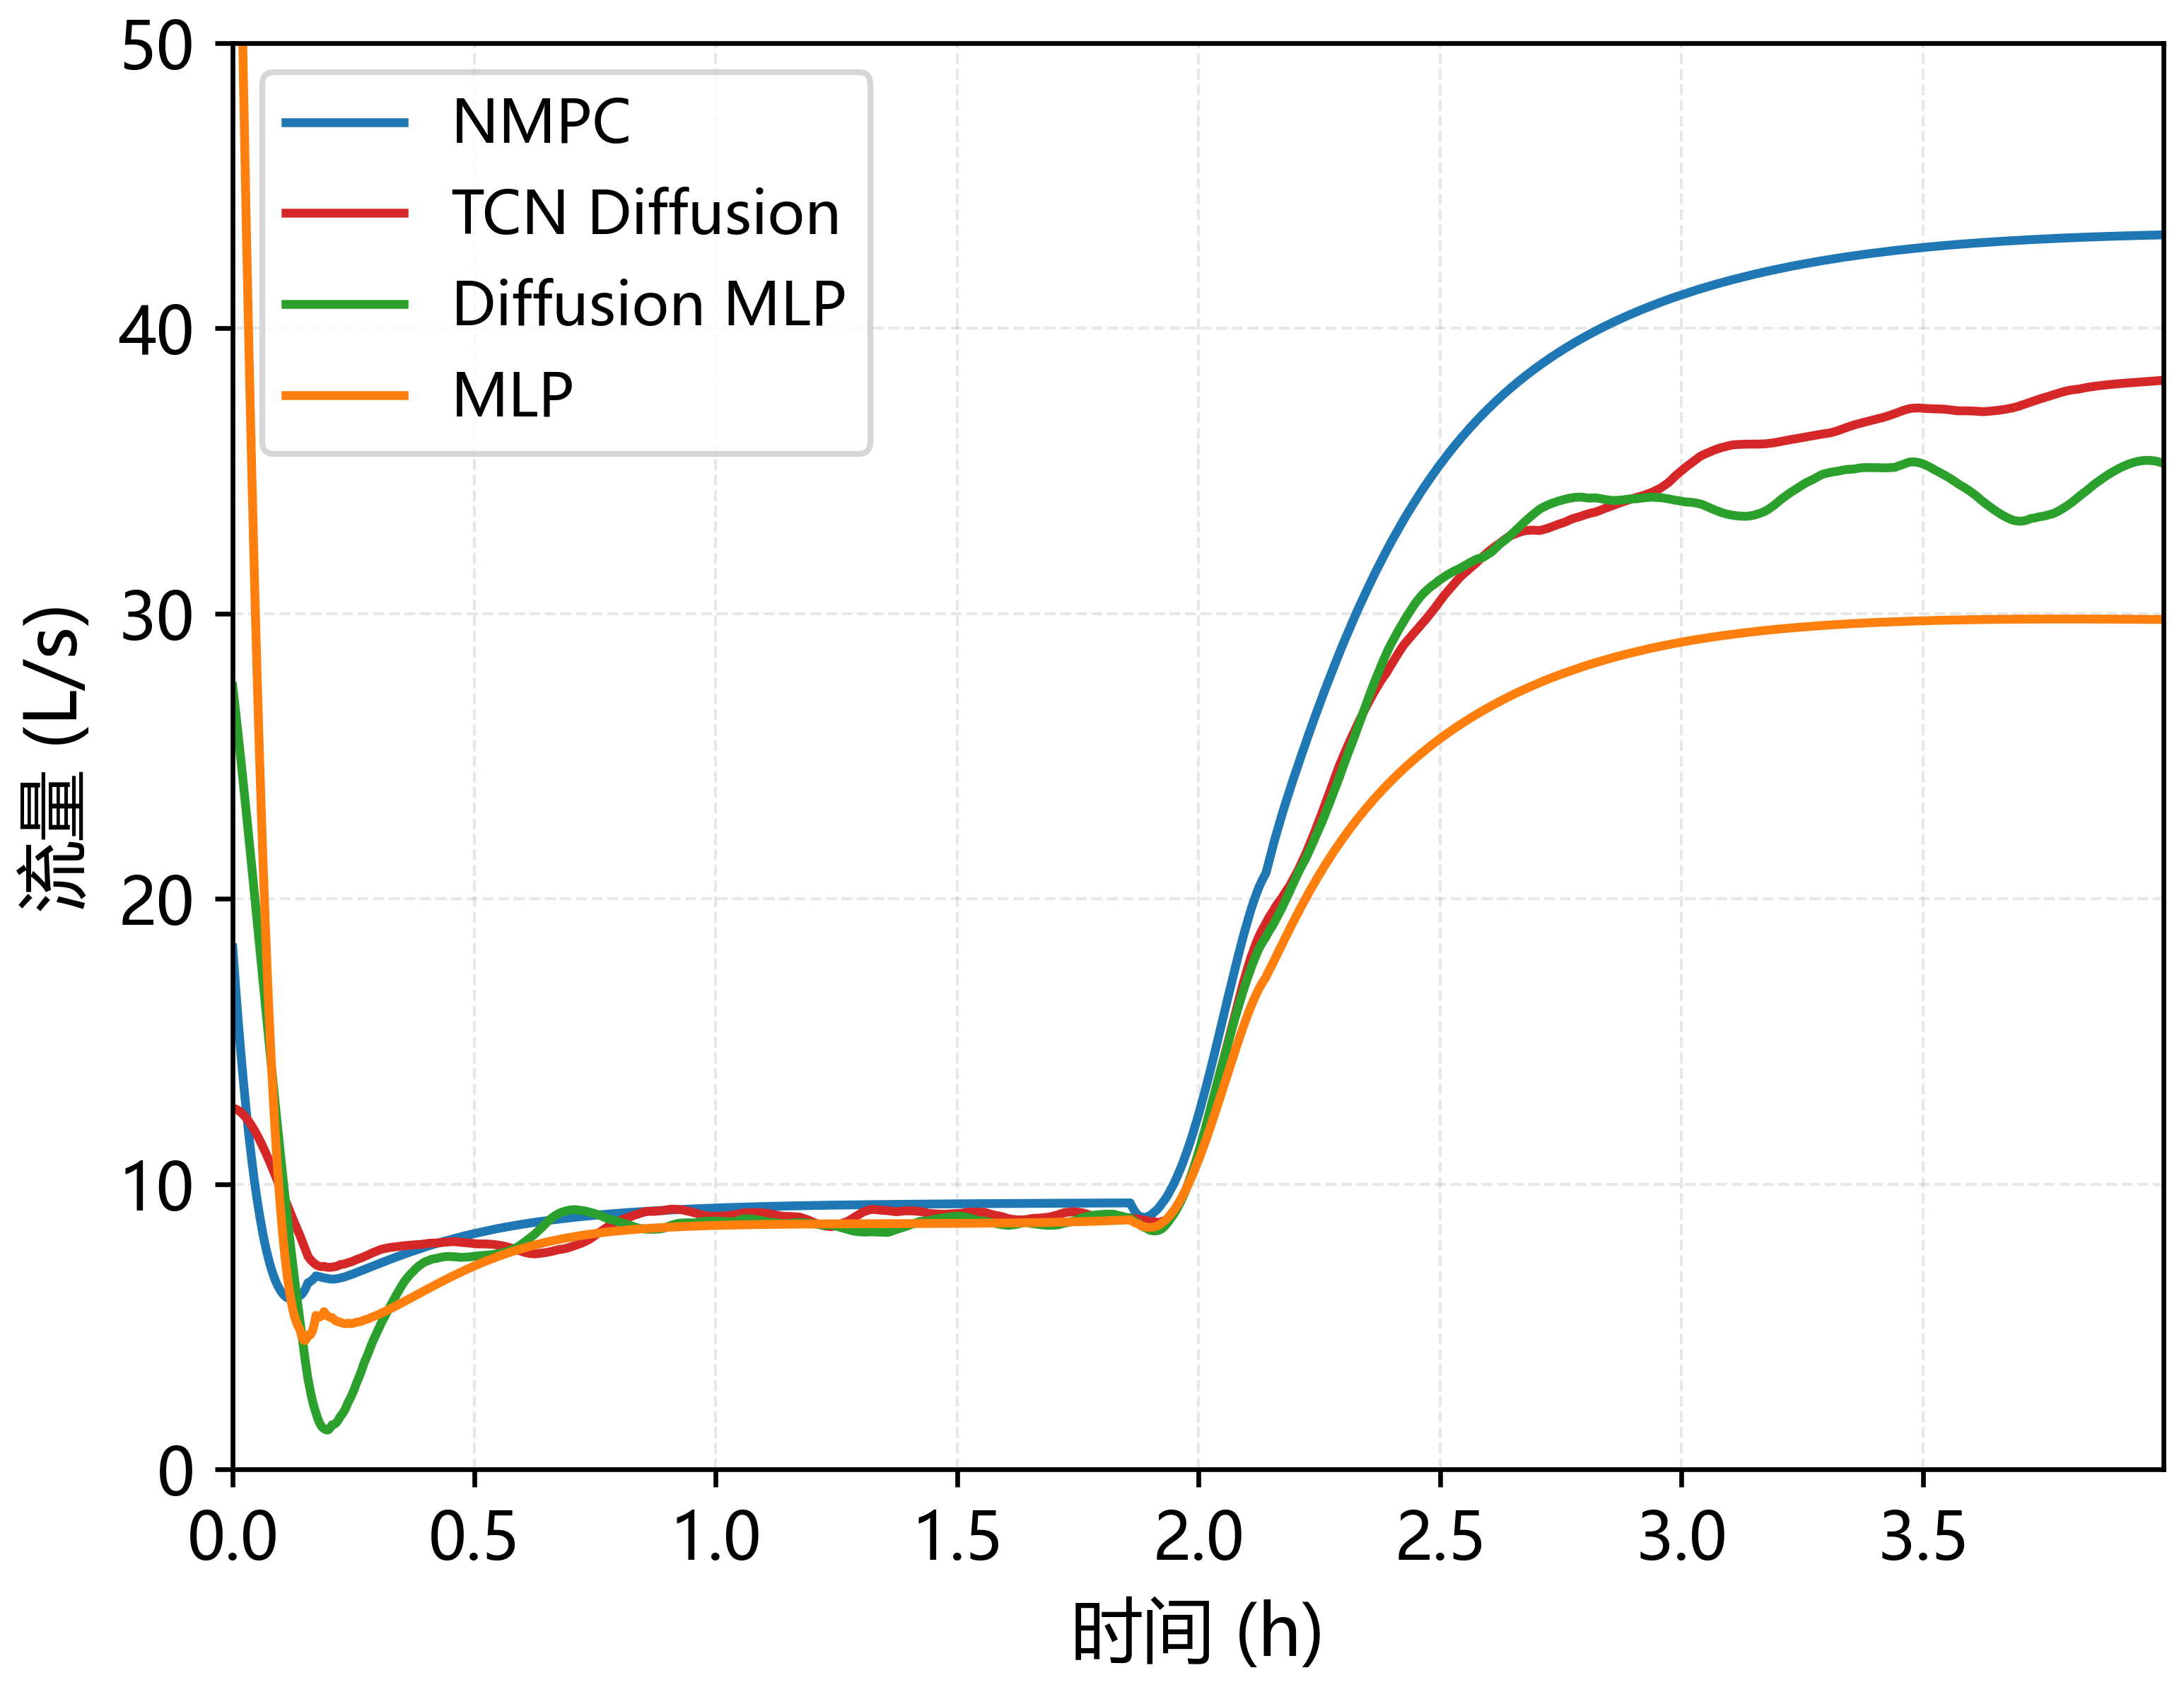
\includegraphics[width=\linewidth]{figures/controller_step_comparison_f.png}
    \caption{}
  \end{subfigure}
  \caption{TCN Diffusion、Diffusion MLP、NMPC与MLP阶跃响应对比}
  \captionsetup{font=normalfont}
  \caption*{(a) 总功率跟踪；(b) 电解槽温度；(c) 氢氧杂质含量；(d) 电解槽电流；(e) 碱液流量；(f) 冷却水流量}
  \label{fig:controller_step_comparison}
\end{figure}

为定量评估四种方法的控制品质并对比其计算效率，基于NMPC目标函数计算累计成本，同时结合单步计算时间基准测试，结果如图~\ref{fig:controller_cost_comparison}所示。
从总成本来看，TCN Diffusion的累计成本最低（6,511），NMPC次之（6,597），Diffusion MLP再次（7,273），MLP最高（7,974）。
MLP总成本显著高于其他方法，根源在于其温度控制品质差导致温度惩罚项大幅累积，同时碱液流量的剧烈振荡也带来了高额的平滑性惩罚；其功率跟踪的微弱优势远不足以弥补上述缺陷。
TCN Diffusion总成本最低，且在温度控制、碱液平滑与生产均衡性上均表现优异，综合控制品质最为均衡。
单步计算时间方面（图~\ref{fig:controller_cost_comparison}(b)），MLP作为最简单的网络结构，单步耗时仅约10.9~ms；Diffusion MLP与TCN Diffusion由于需要多次去噪迭代，计算时间分别为约155~ms和177~ms，但仍比NMPC的在线优化求解快约两个数量级；NMPC的单步计算时间高达约17.6~s，这使其难以满足实时控制需求。
结果表明，基于扩散模型的策略在保持接近NMPC控制品质的同时，将单步计算时间从秒级降低到毫秒级，具备显著的实时应用优势。

\begin{figure}[!htbp]
  \centering
  \begin{subfigure}{0.48\textwidth}
    \centering
    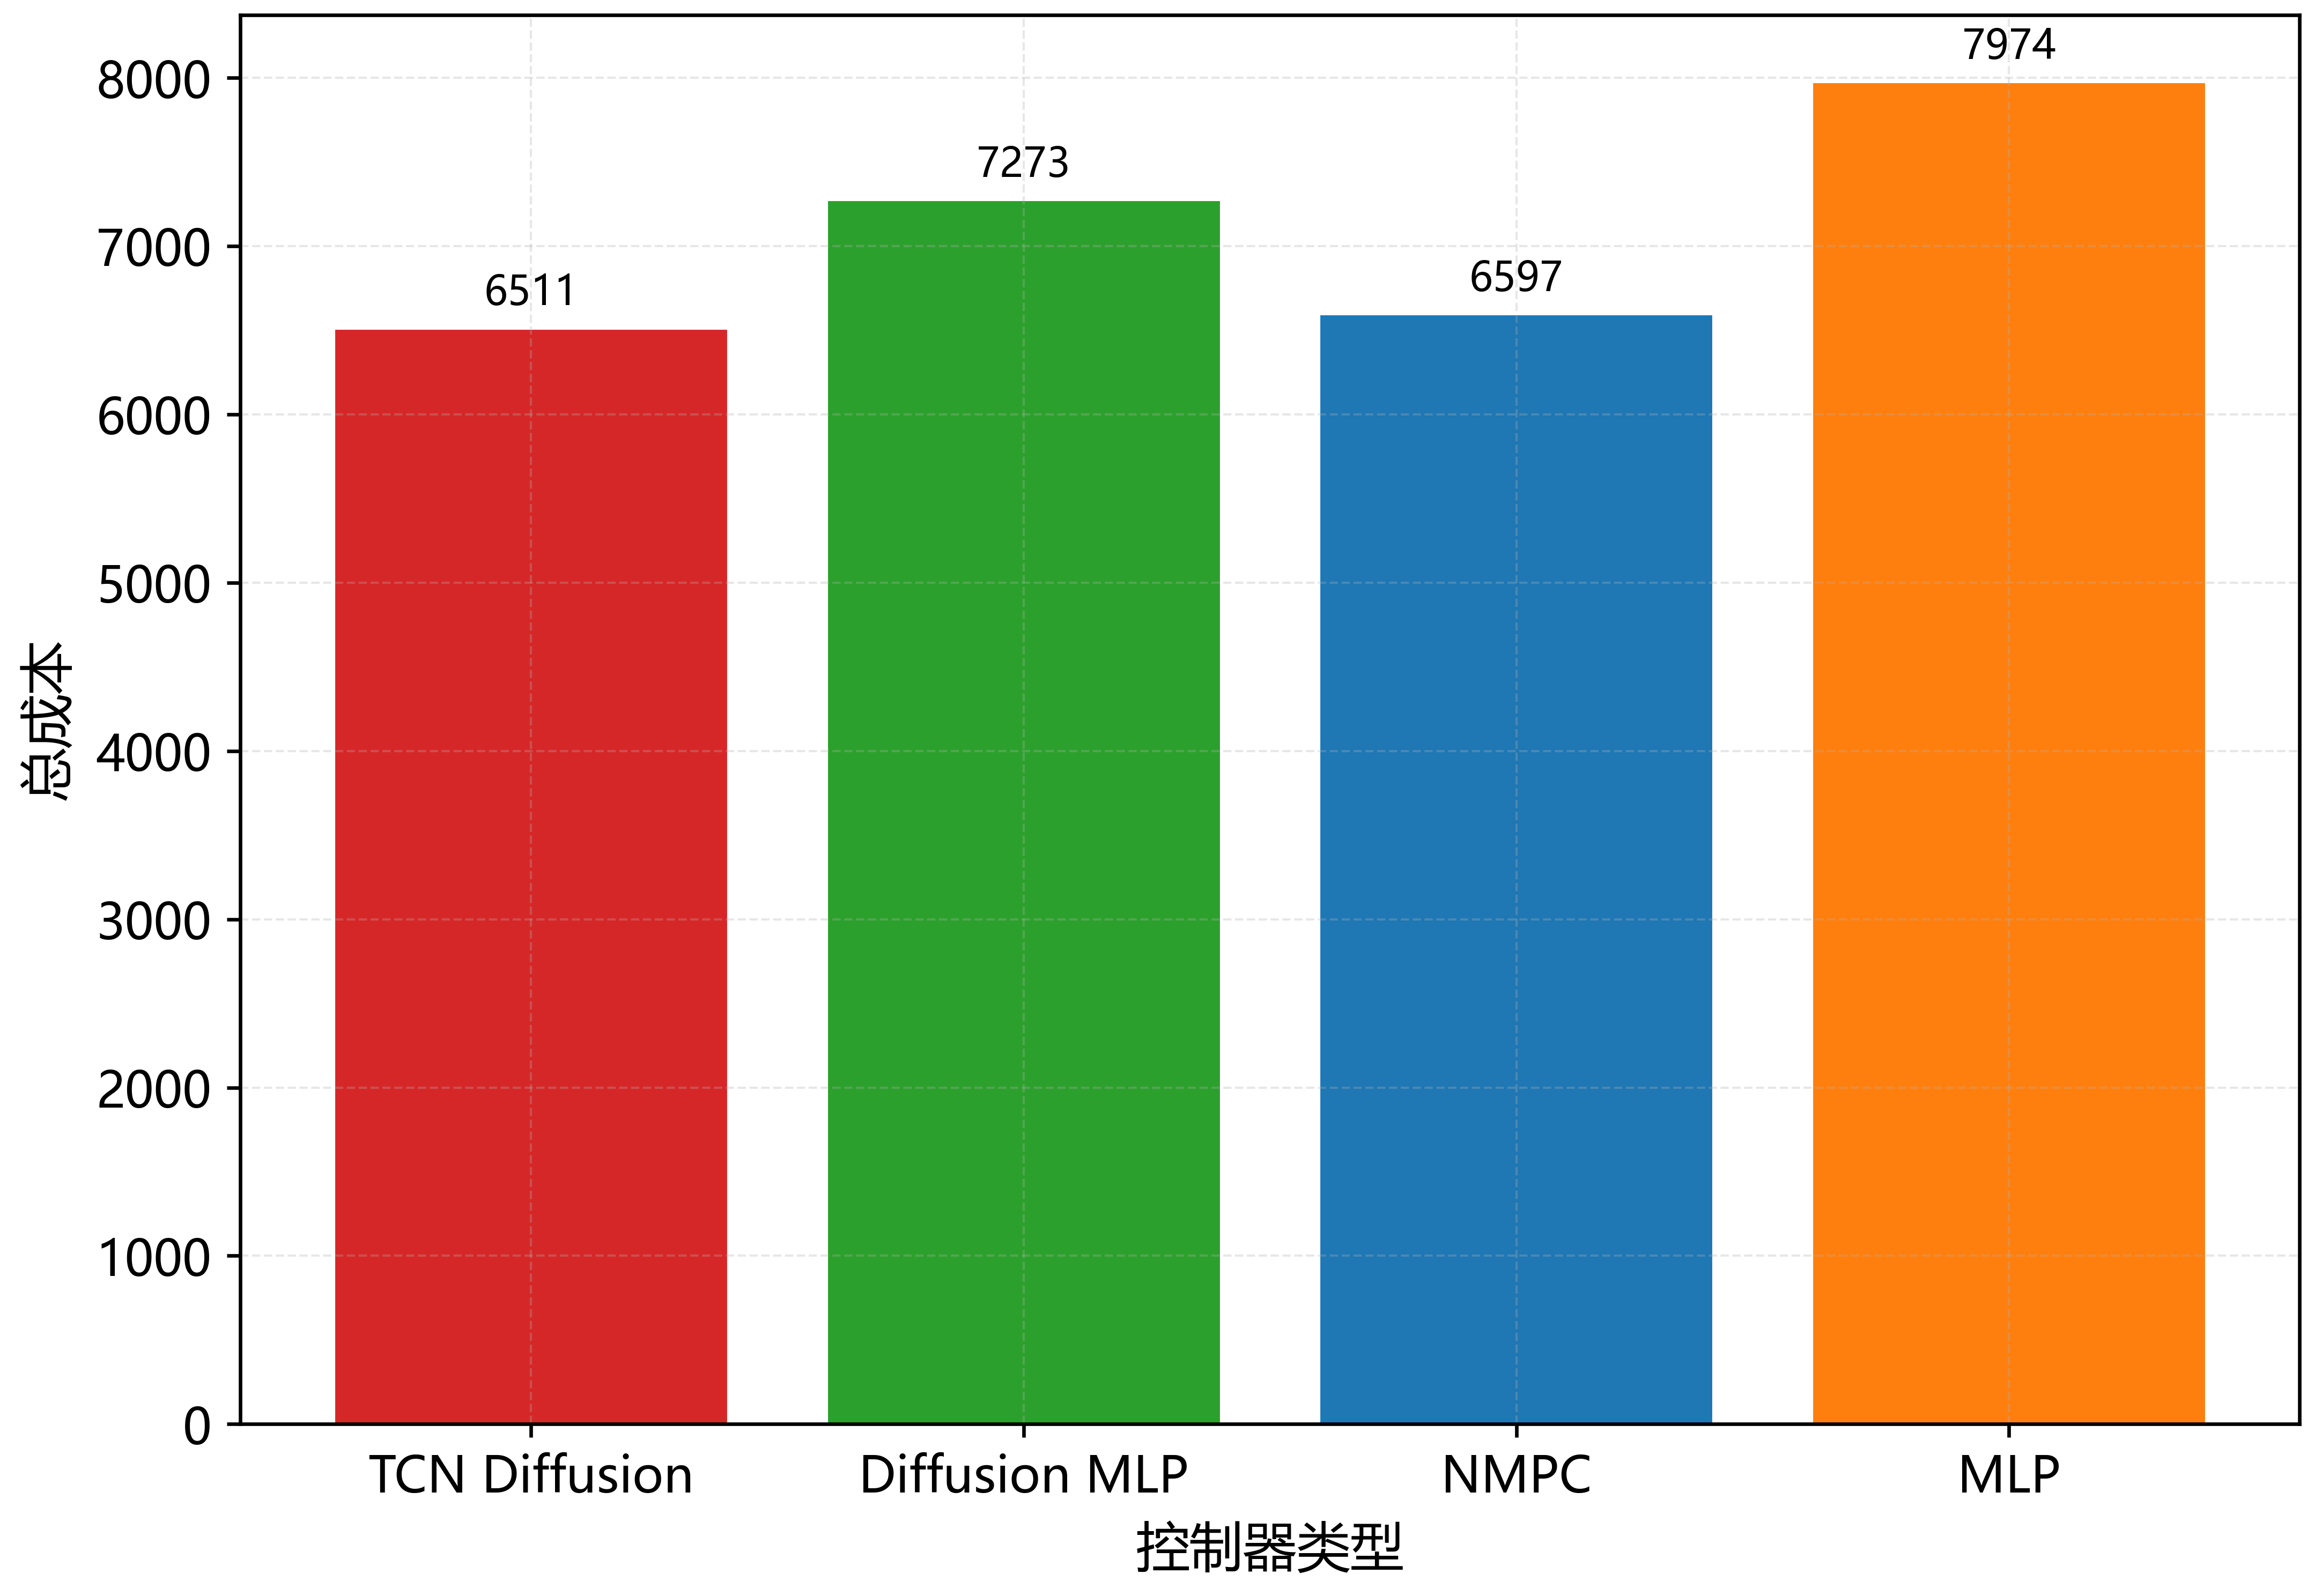
\includegraphics[width=\linewidth]{figures/controller_cost_comparison_a.png}
    \caption{}
  \end{subfigure}
  \hfill
  \begin{subfigure}{0.48\textwidth}
    \centering
    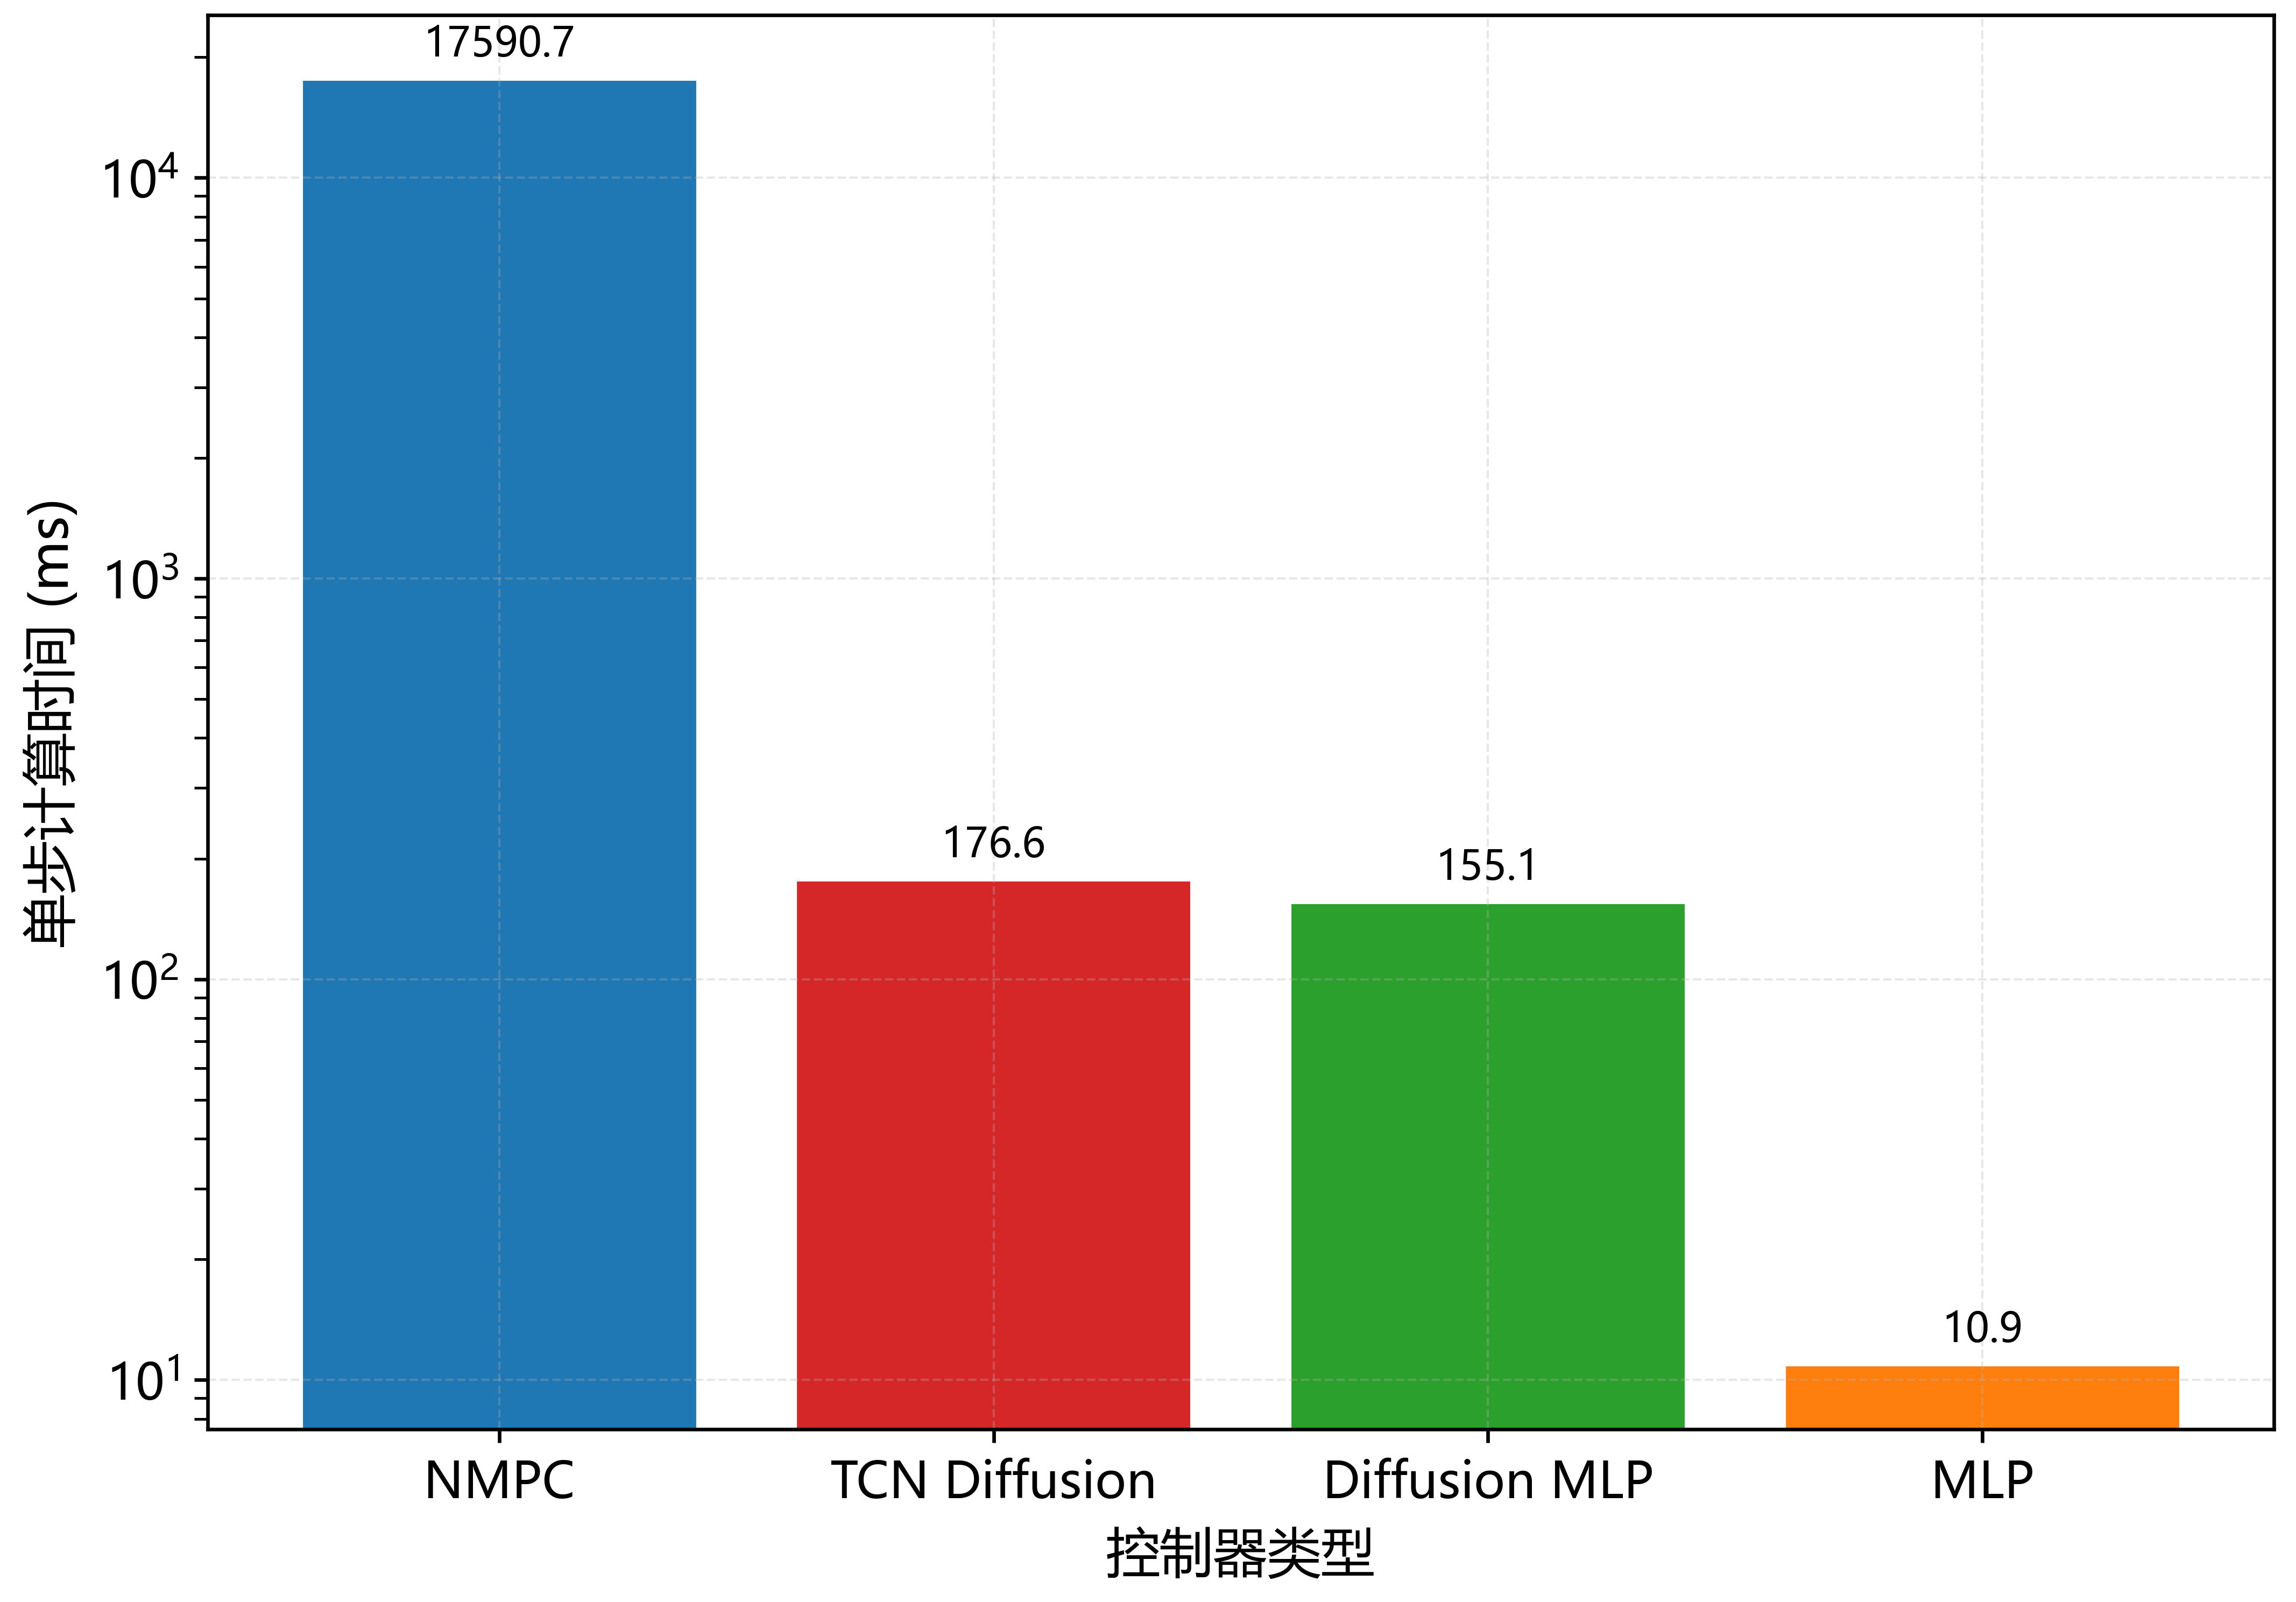
\includegraphics[width=\linewidth]{figures/controller_cost_comparison_b.png}
    \caption{}
  \end{subfigure}
  \caption{四种控制方法总成本及单步计算时间对比}
  \captionsetup{font=normalfont}
  \caption*{(a) 各成本分量对比；(b) 单步计算时间对比}
  \label{fig:controller_cost_comparison}
\end{figure}

\subsubsection{风电场景实验对比}

阶跃响应实验验证了功率突变工况下的动态特性，而持续波动的风电场景则进一步检验控制器的稳态跟踪品质与长期运行鲁棒性。为此，基于某风电场实测功率曲线开展24小时闭环仿真对比实验，对象包括TCN Diffusion、Diffusion MLP、NMPC与MLP四种控制器，其中NMPC作为优化基准，MLP作为无扩散过程的纯神经网络基线，Diffusion MLP与TCN Diffusion则分别检验扩散去噪机制与时序卷积结构的贡献。仿真中真实风电功率在0--40~MW范围内剧烈波动，包含大量陡升/陡降与频繁变向工况，对控制器的动态响应与约束保持能力提出较高要求。评价指标涵盖功率跟踪精度（RMSE、MAE、最大偏差）、温度控制品质（MAE、波动范围）、HTO安全性（峰值、99分位值）以及控制量平滑性（碱液流量与冷却水流量的极差与标准差）。

图~\ref{fig:controller_wind_comparison} 展示了四种方法在24小时风电跟踪场景下的闭环响应。功率跟踪方面，四种方法均能跟踪风电功率的剧烈波动，整体RMSE均在6.10~MW左右，MAE约5.22--5.31~MW，最大跟踪误差约8.64~MW，整体精度相近。这说明在功率波动相对平稳、不存在剧烈阶跃突变时，各方法的功率跟踪能力差异不大。温度控制方面，四种方法均能将电解槽温度控制在安全范围内，但表现分化明显：NMPC凭借在线优化与完整模型信息取得最优温度精度（MAE~0.229~K）；纯MLP在持续波动场景下温度MAE仅0.233~K，已接近NMPC甚至优于TCN Diffusion（0.238~K），这与阶跃工况中其1.42~K的较差表现形成鲜明对比，表明纯前馈网络对平稳波动的拟合能力尚可，但对剧烈瞬态的预测仍存在显著滞后；Diffusion MLP因MLP主干网络时序建模能力不足，温度偏差最大（0.328~K）。HTO安全方面，所有方法均能将气相氢气浓度控制在2\%安全阈值以下，峰值均为0.87\%，99分位值在0.63\%--0.64\%之间，安全裕度充足。控制量平滑性方面，碱液流量呈现显著分化：Diffusion MLP的碱液流量脉动最大（极差14.32~L/s），因其MLP主干难以学习气液分离动态的长期惯性；TCN Diffusion则凭借时序卷积结构实现了最平滑的碱液调节（极差5.70~L/s）；纯MLP的碱液平滑性尚可（极差7.50~L/s），但其冷却水流量波动范围最广（极差70.9~L/s），显著高于NMPC（55.9~L/s），反映出纯前馈结构在多变量协调控制上的不足——电流与碱液流量的决策相对独立，导致热管理回路与功率跟踪回路之间缺乏有效耦合，冷却水调节呈现高频振荡。

\begin{figure}[!htbp]
  \centering
  \begin{subfigure}{0.48\textwidth}
    \centering
    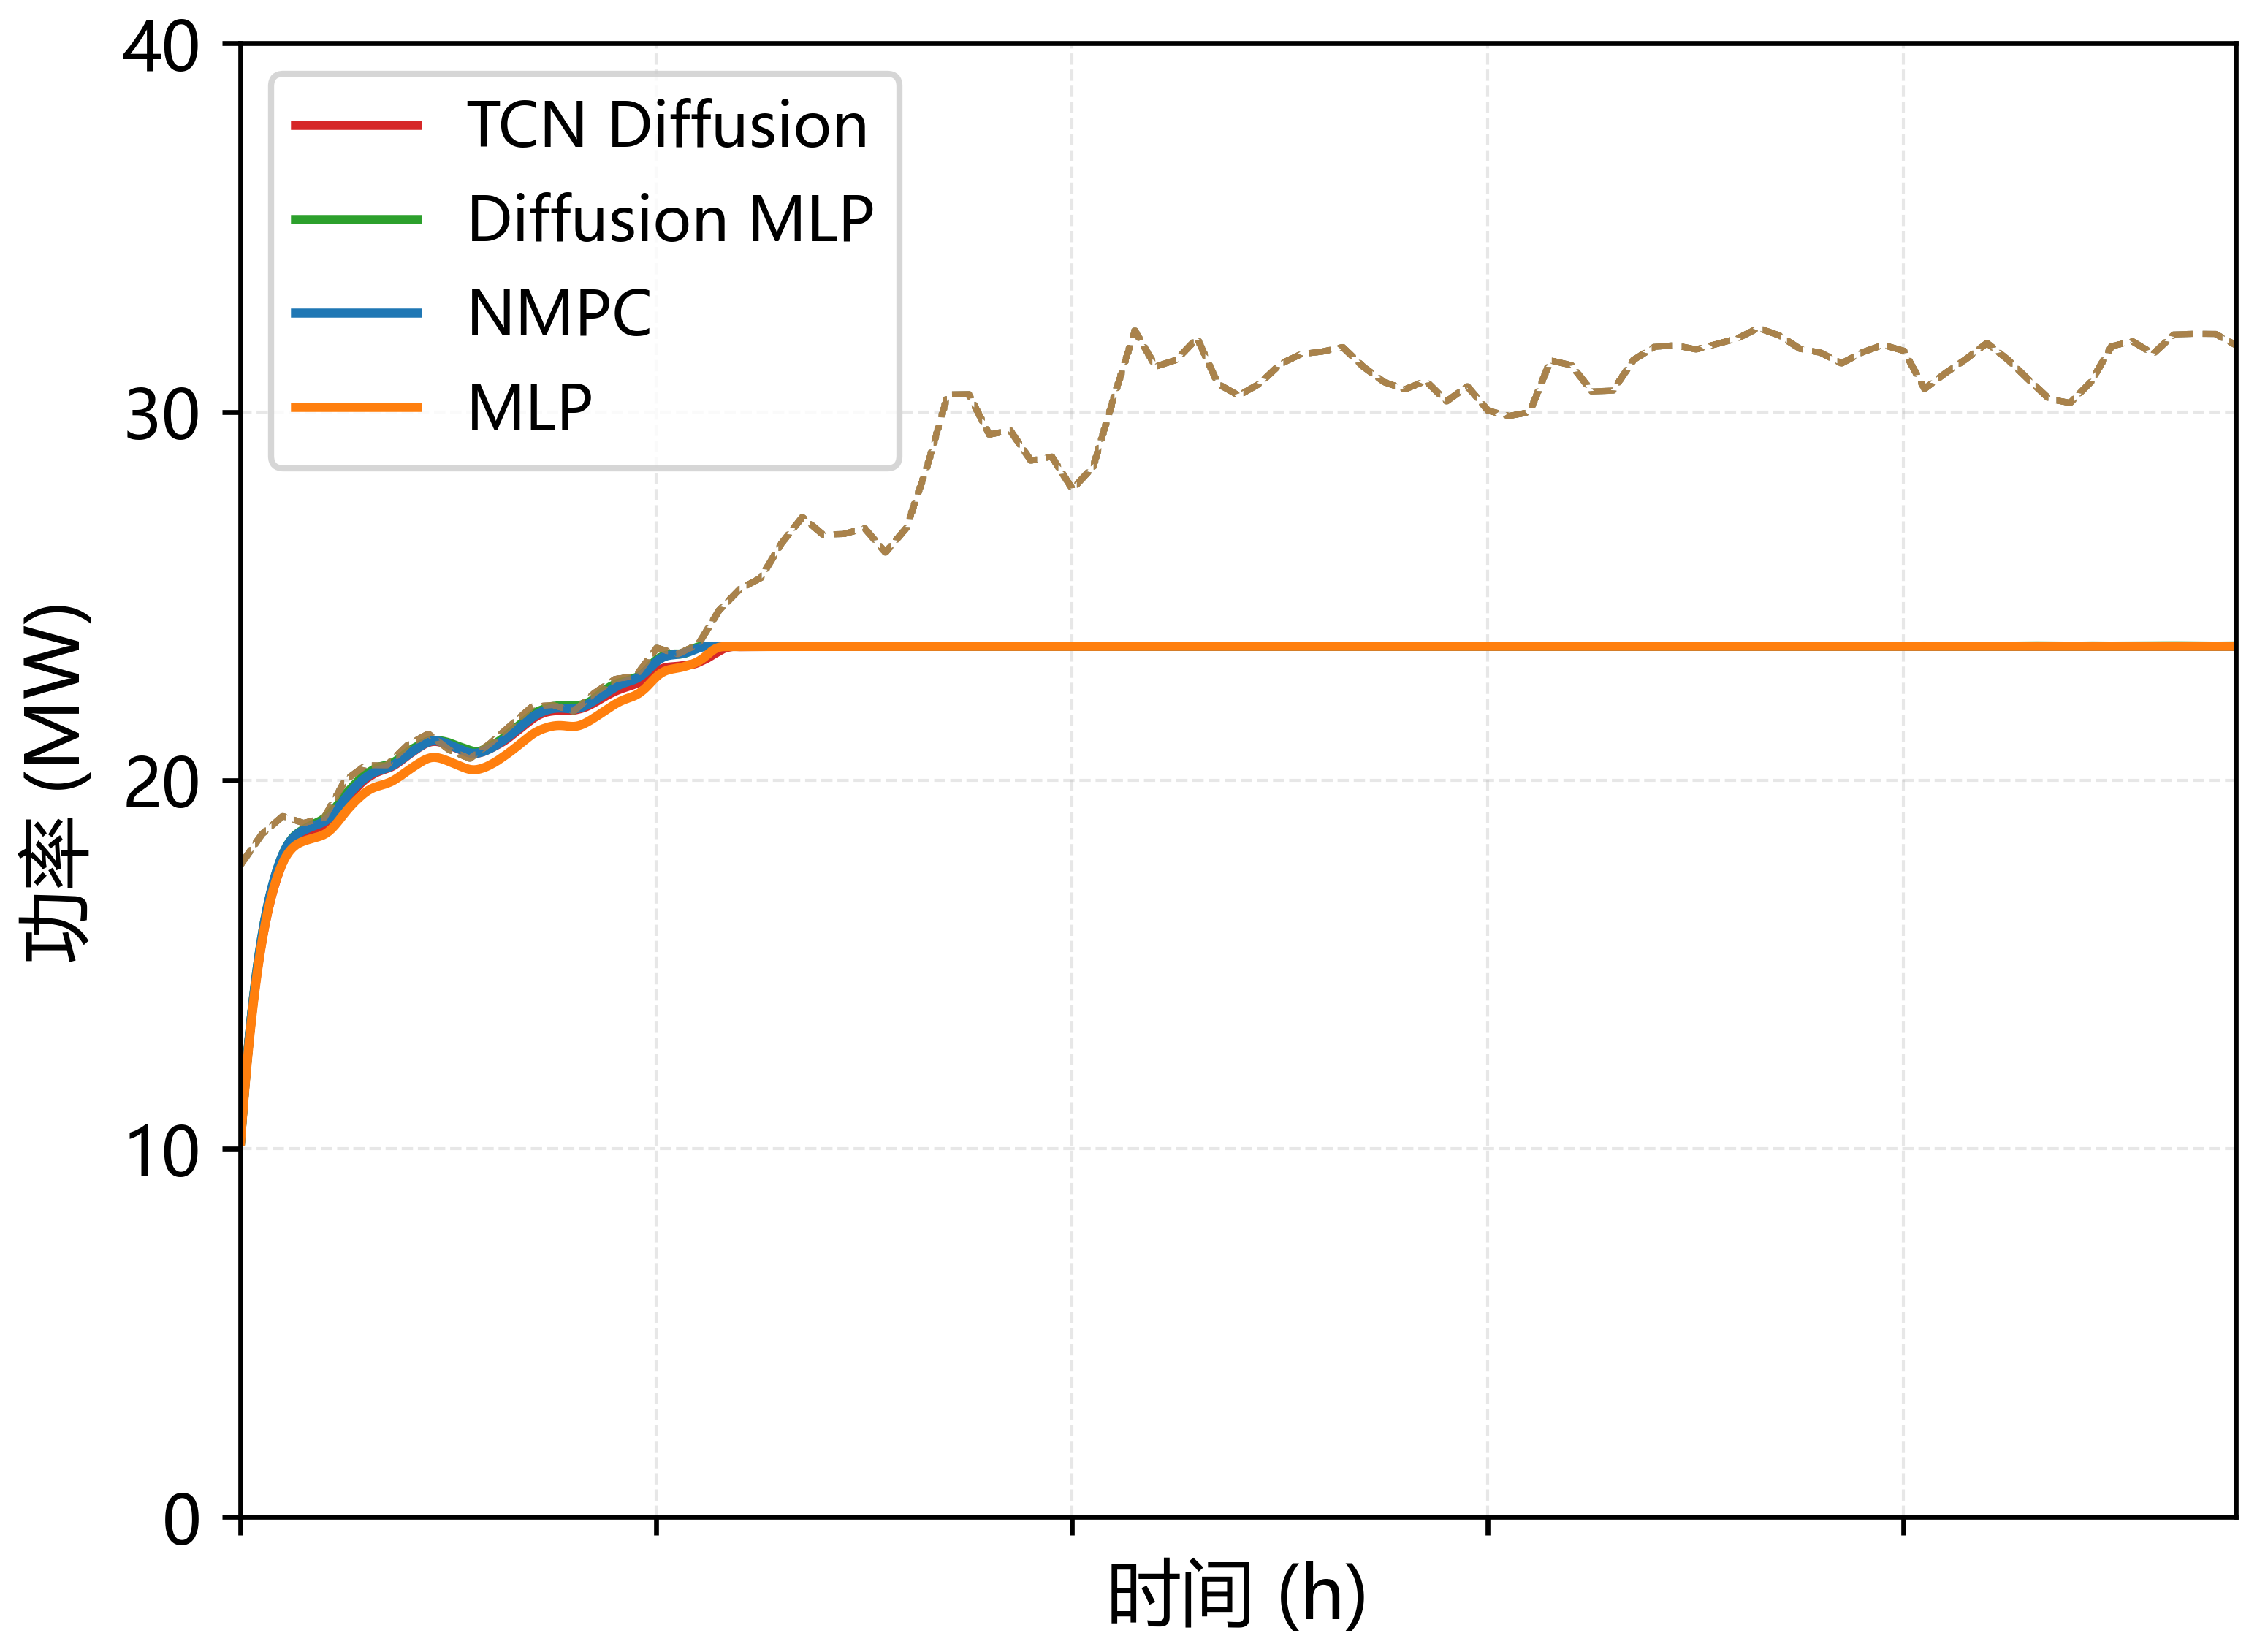
\includegraphics[width=\linewidth]{figures/controller_wind_comparison_a.png}
    \caption{}
  \end{subfigure}
  \hfill
  \begin{subfigure}{0.48\textwidth}
    \centering
    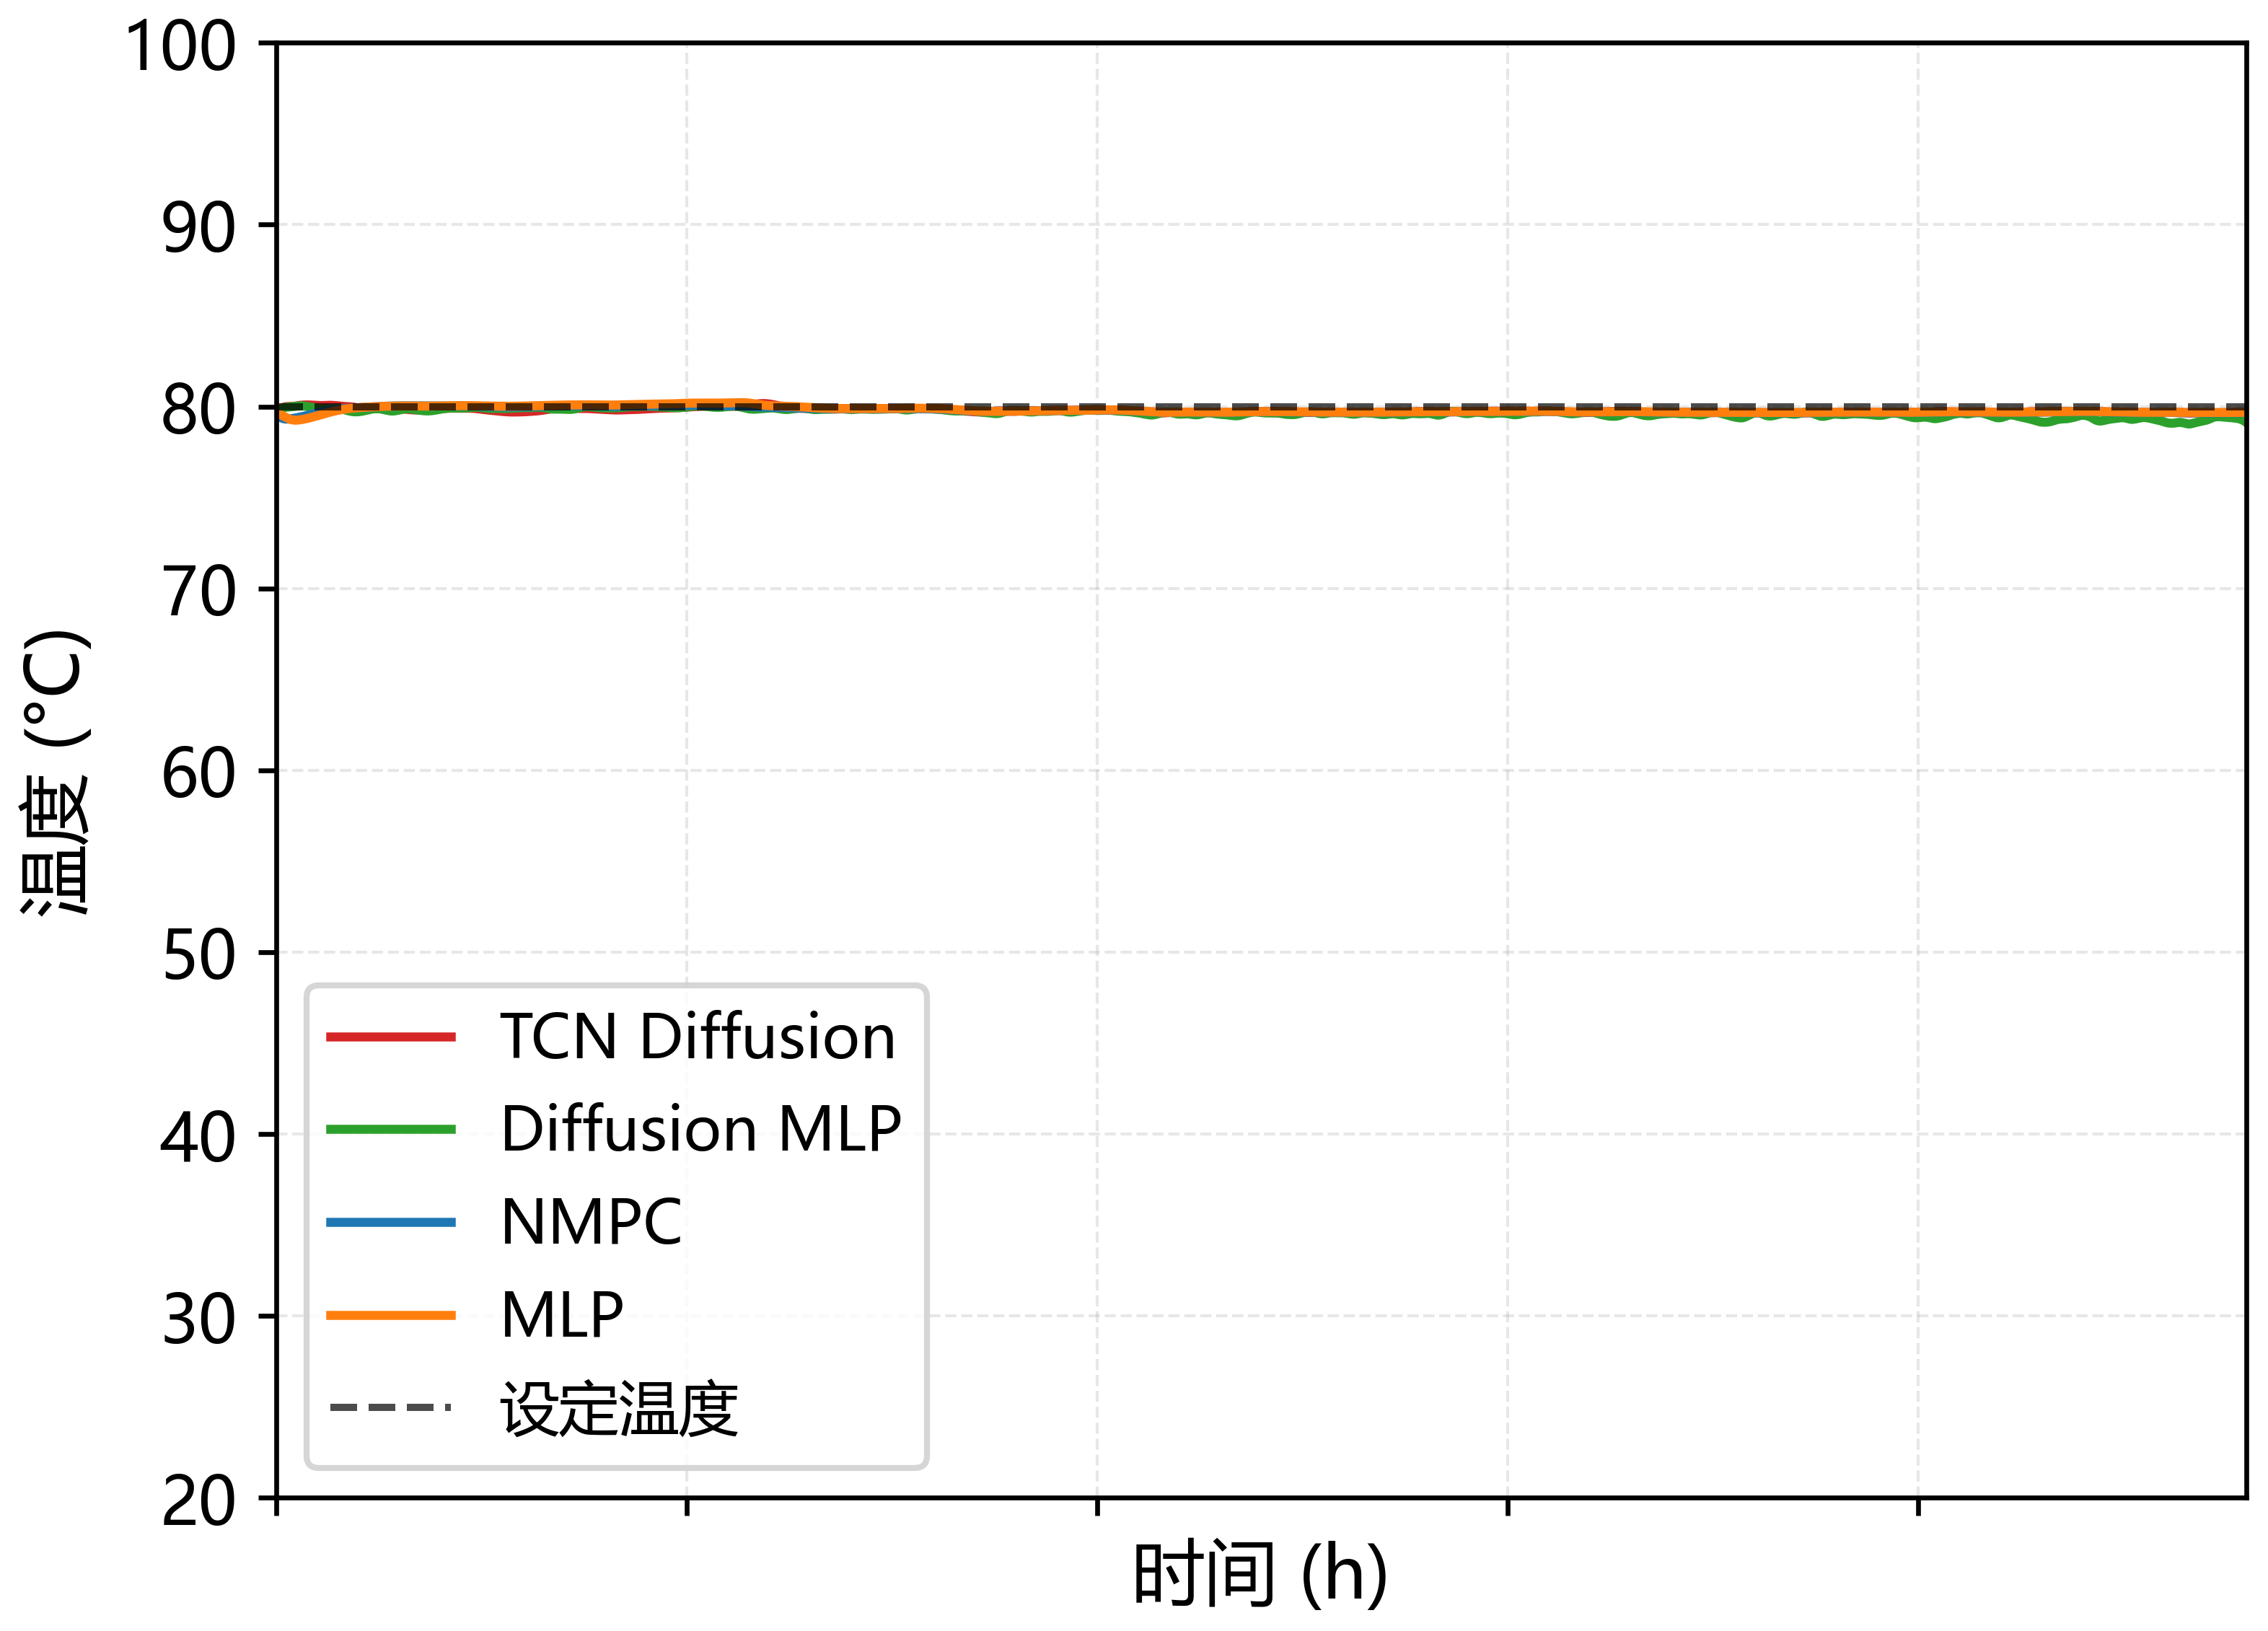
\includegraphics[width=\linewidth]{figures/controller_wind_comparison_b.png}
    \caption{}
  \end{subfigure}

  \begin{subfigure}{0.48\textwidth}
    \centering
    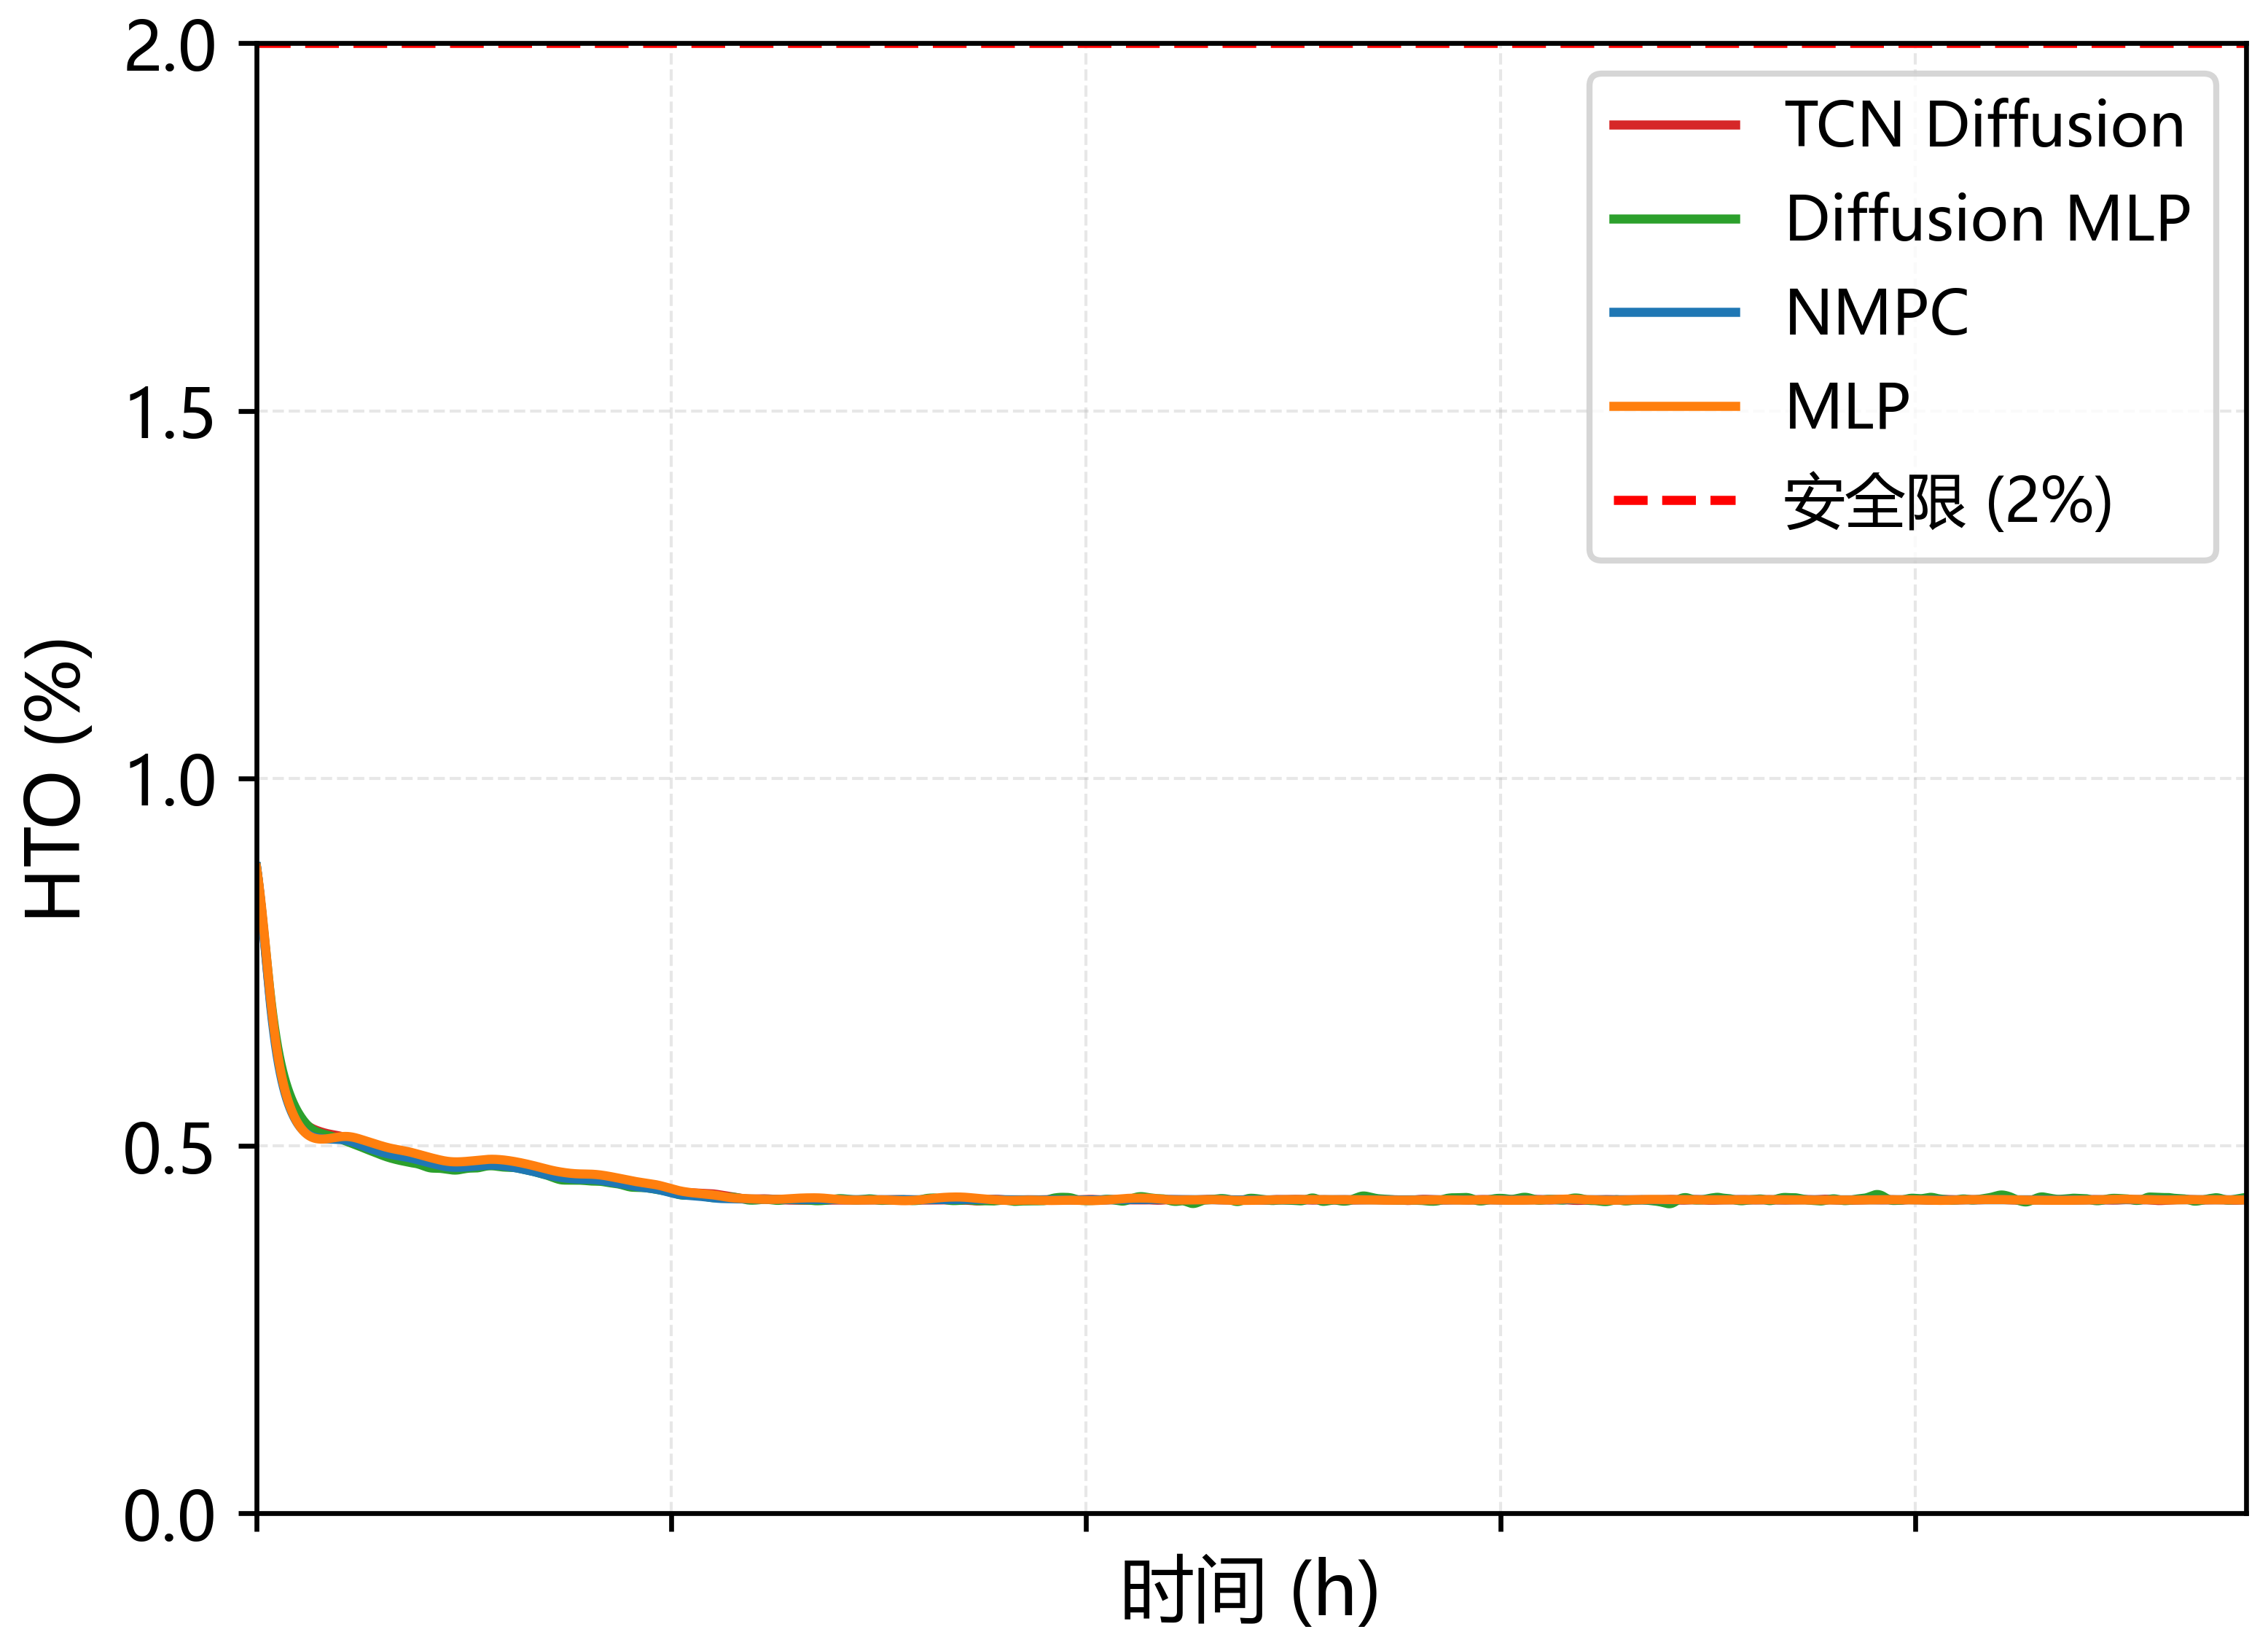
\includegraphics[width=\linewidth]{figures/controller_wind_comparison_c.png}
    \caption{}
  \end{subfigure}
  \hfill
  \begin{subfigure}{0.48\textwidth}
    \centering
    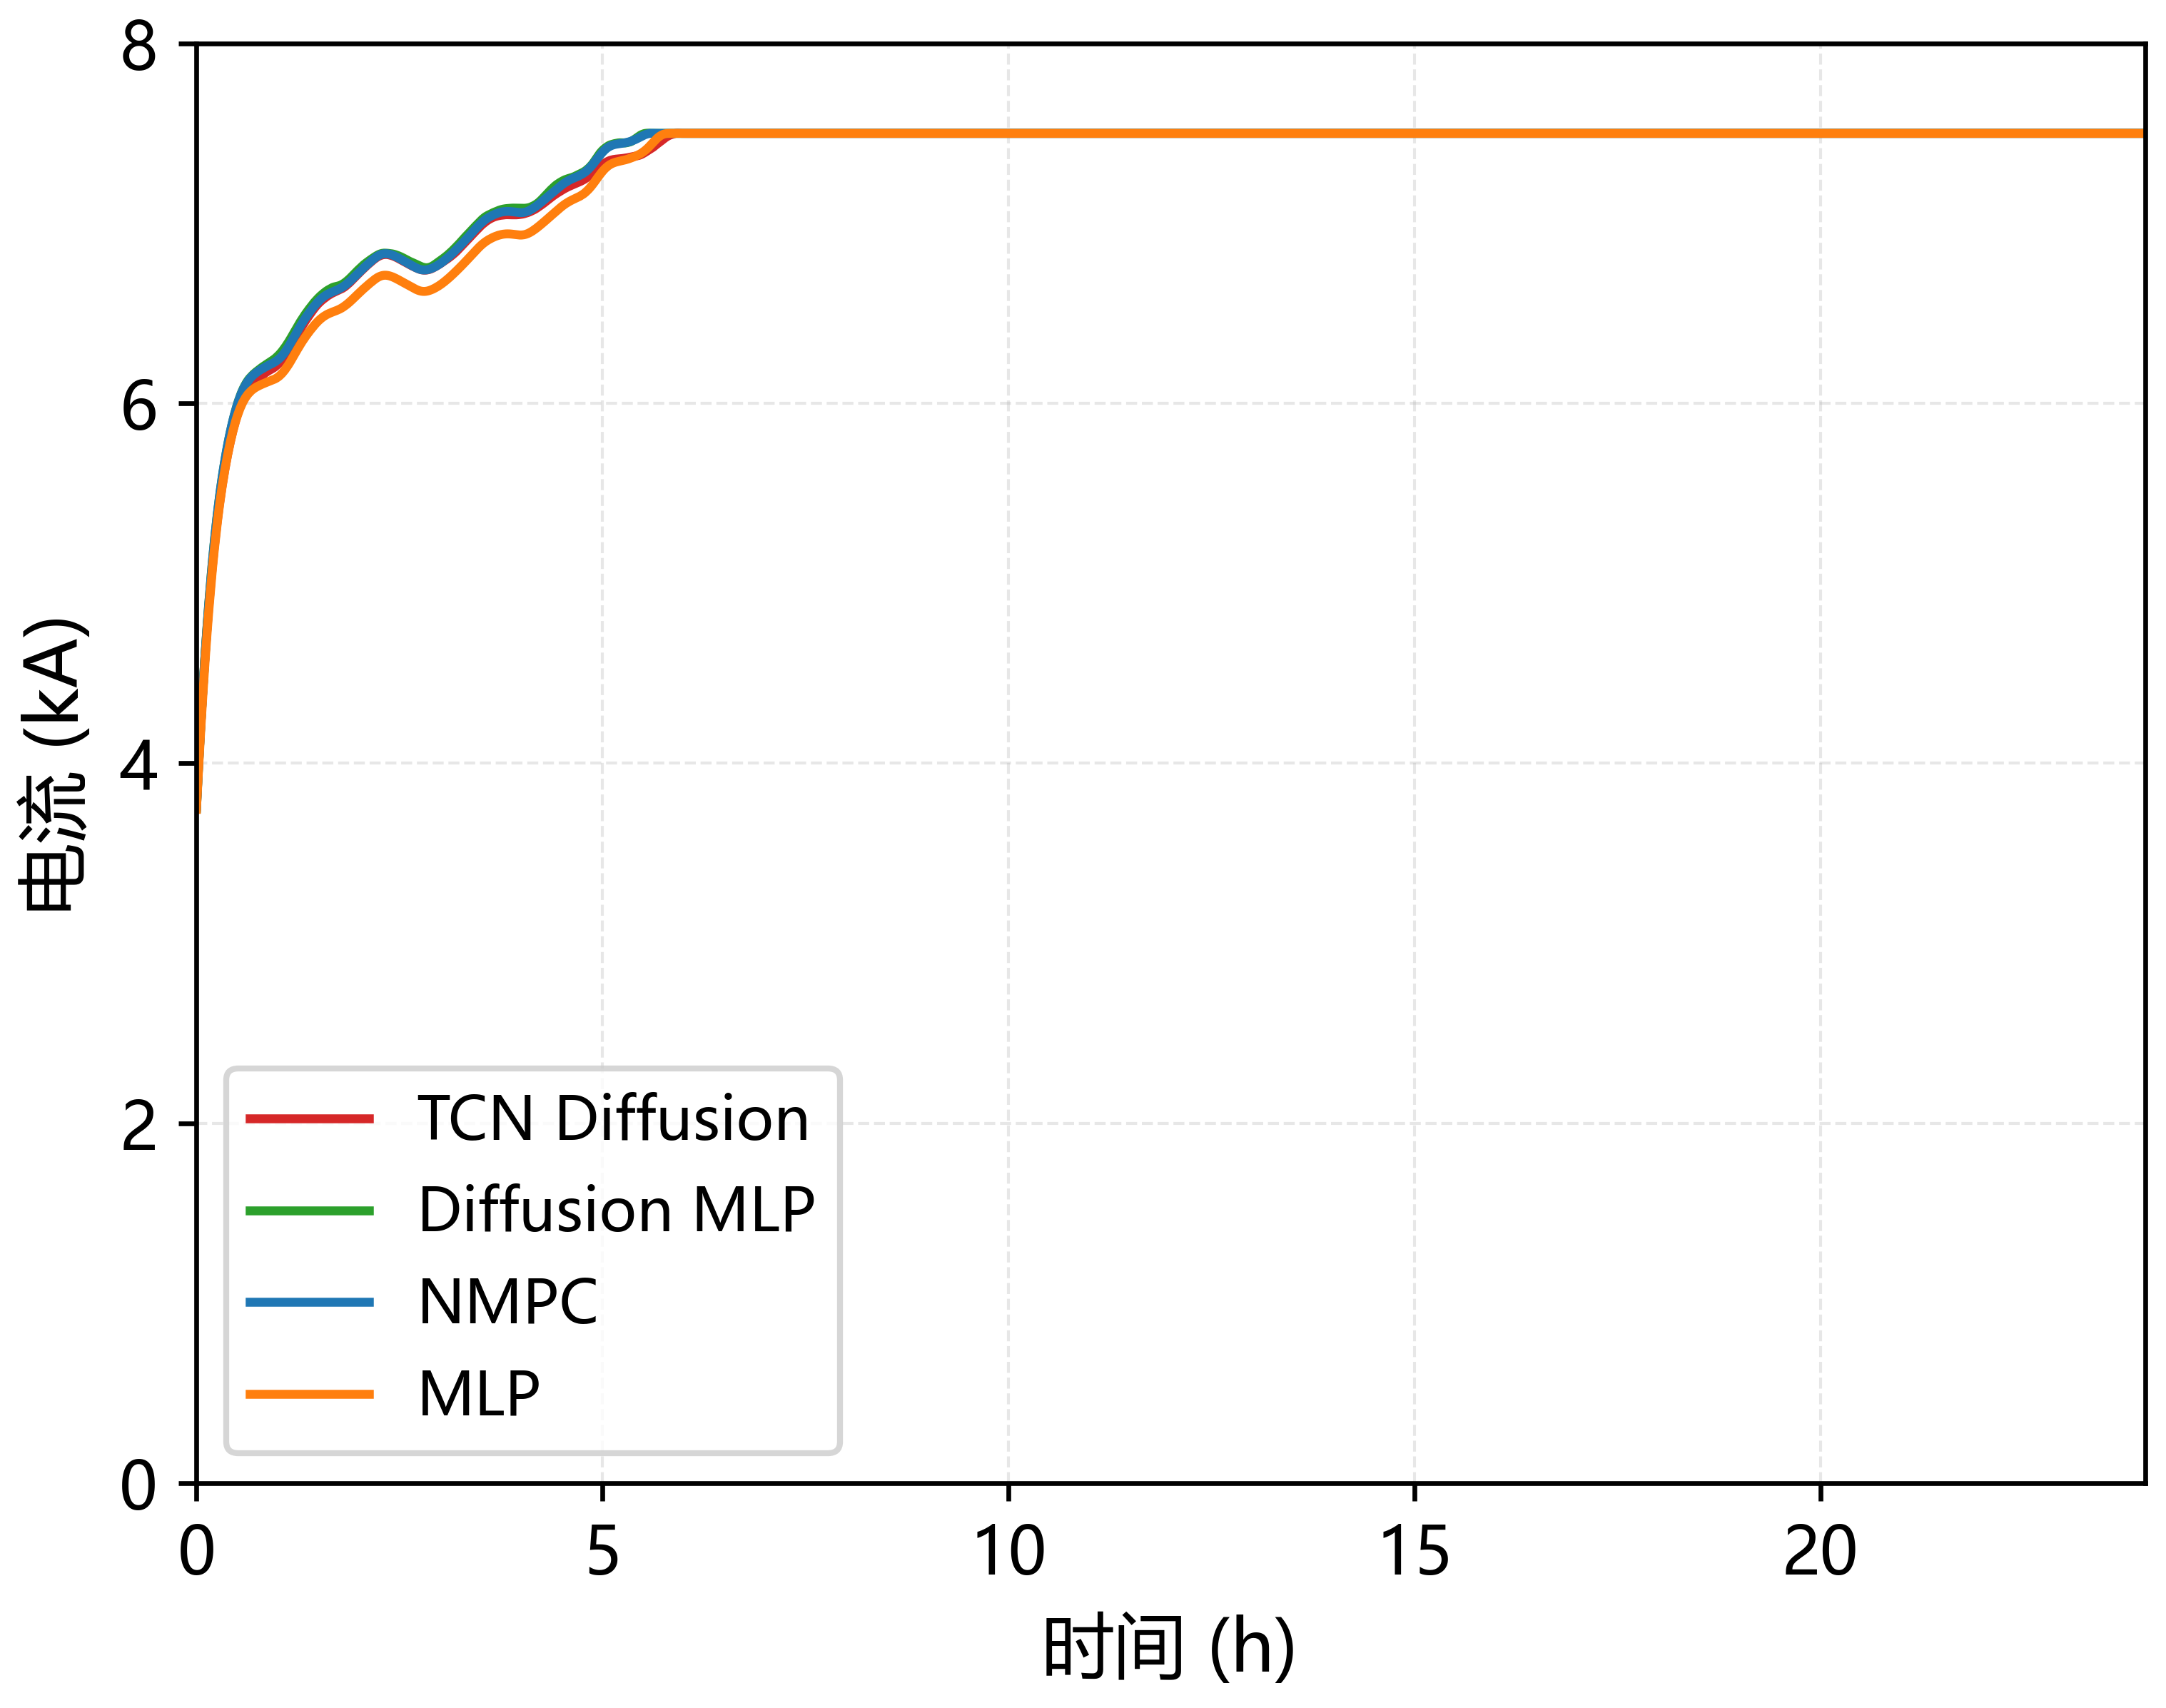
\includegraphics[width=\linewidth]{figures/controller_wind_comparison_d.png}
    \caption{}
  \end{subfigure}

  \begin{subfigure}{0.48\textwidth}
    \centering
    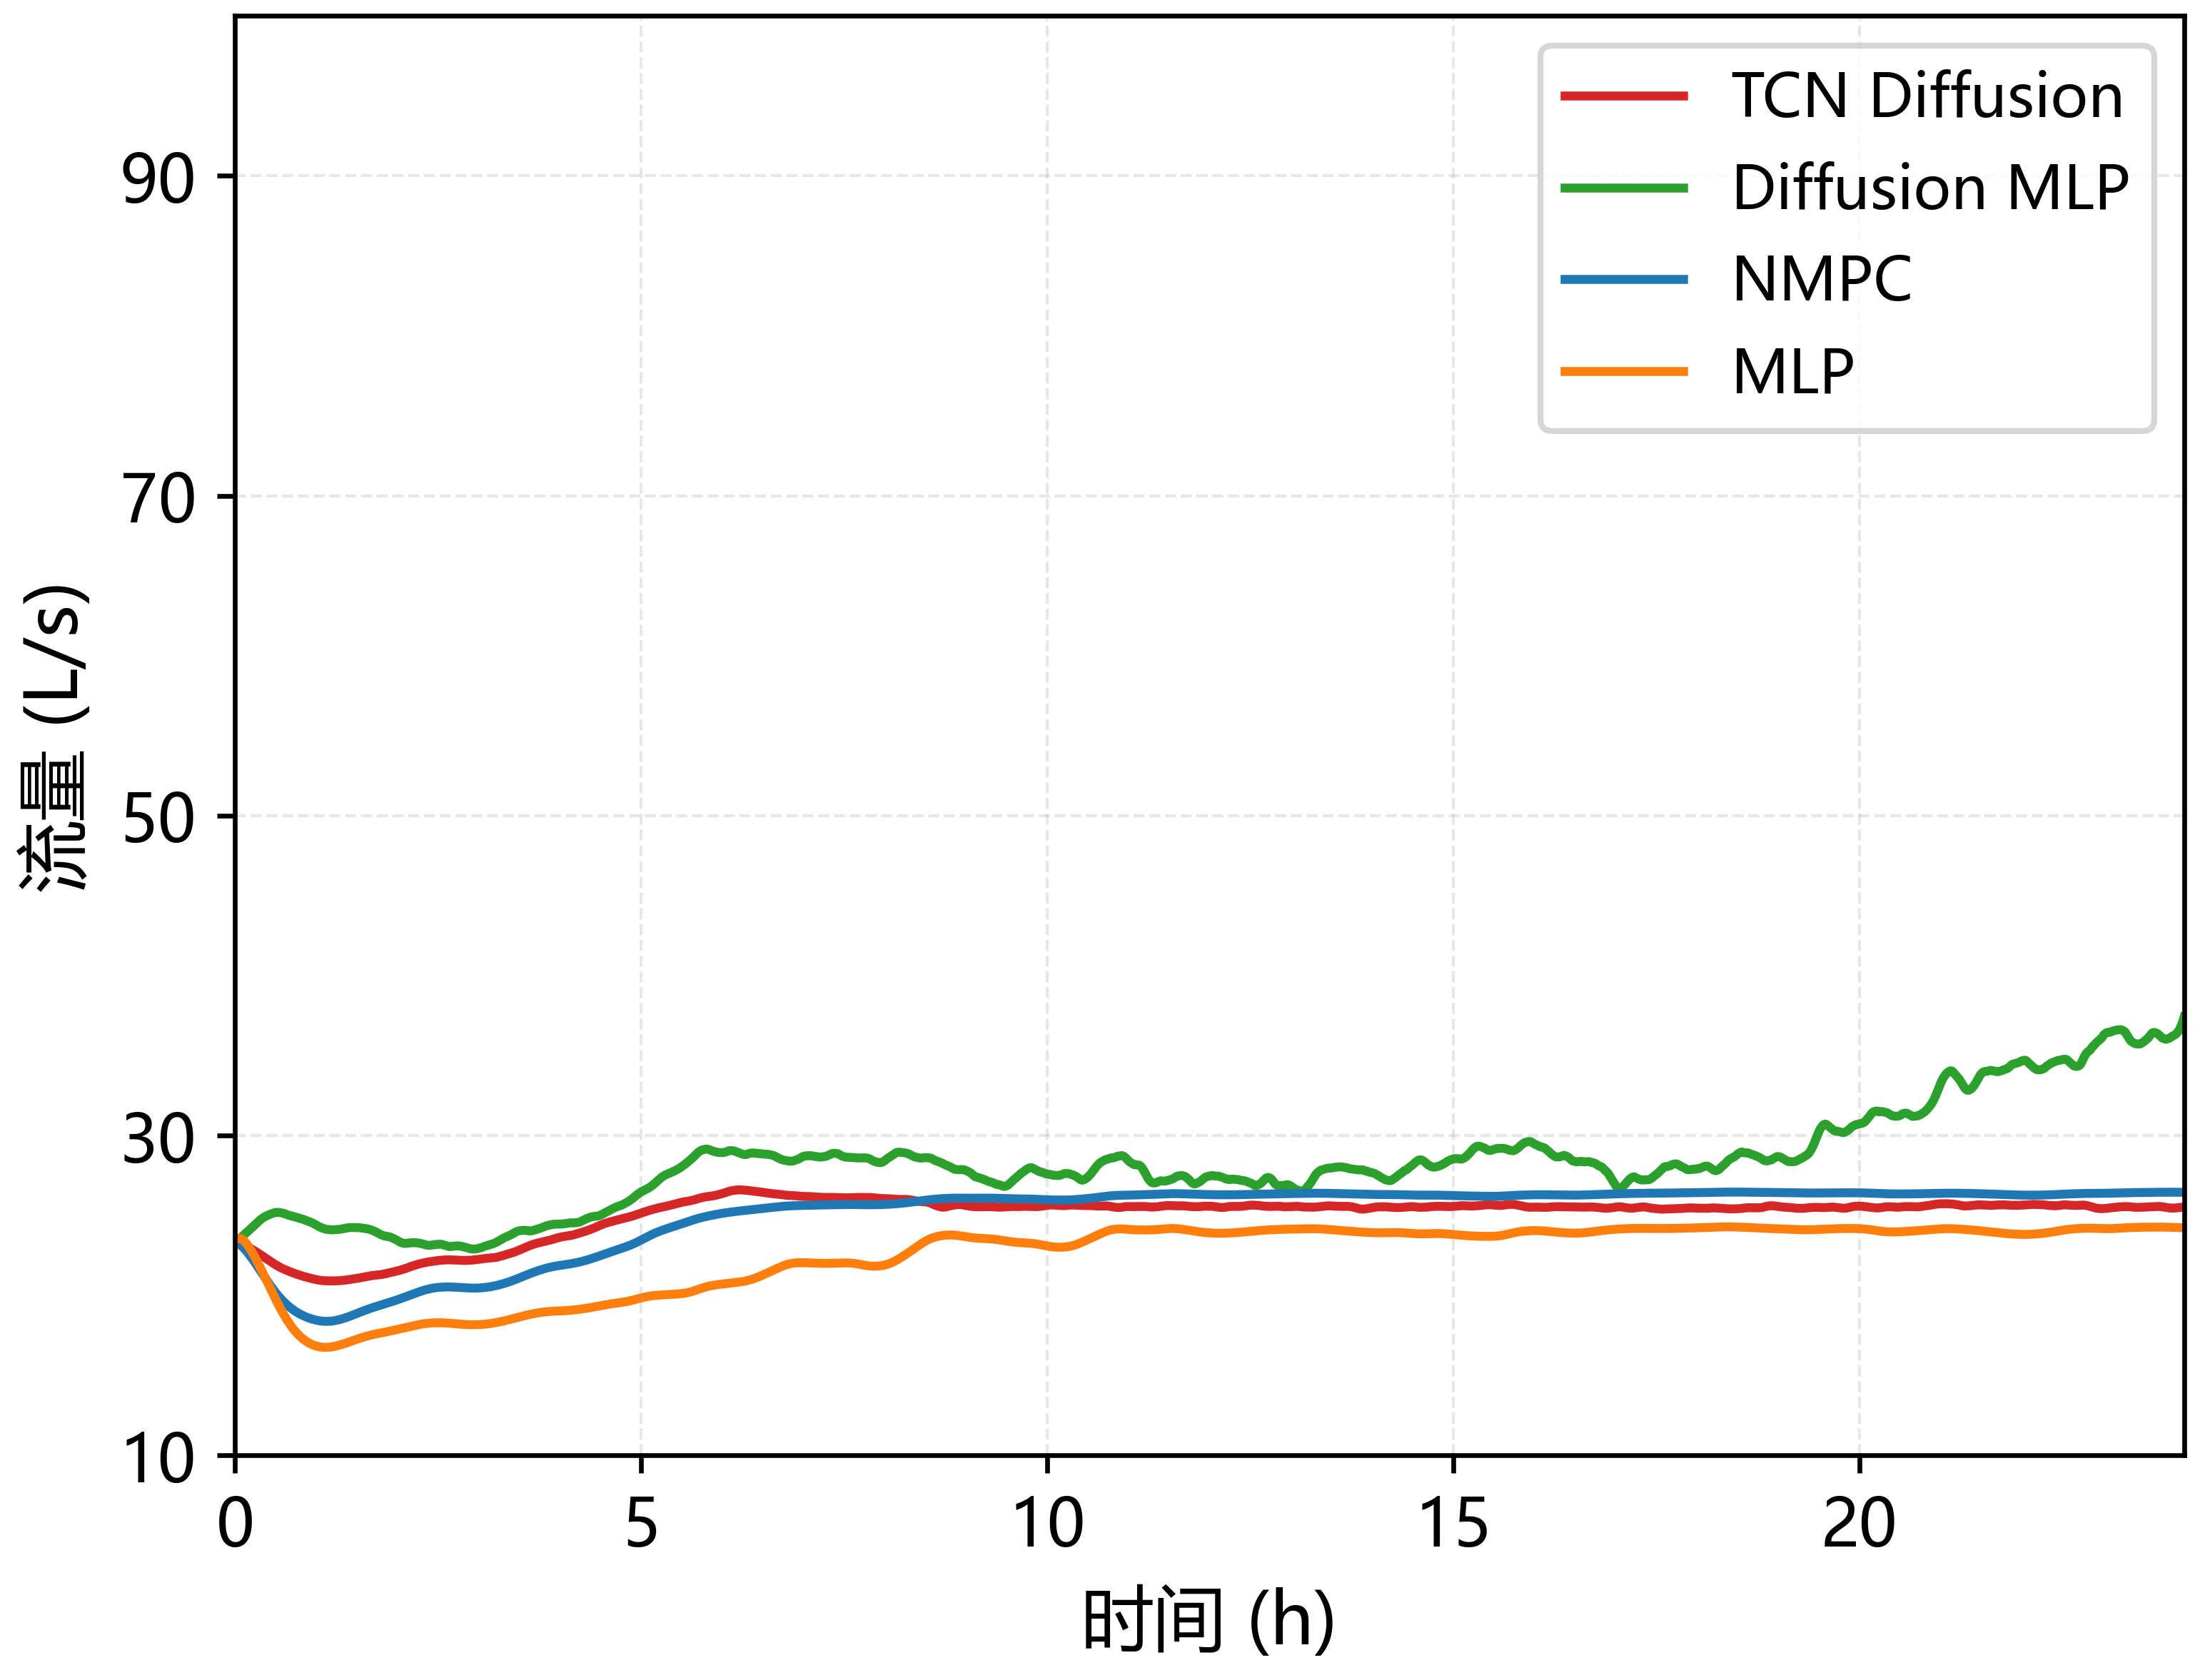
\includegraphics[width=\linewidth]{figures/controller_wind_comparison_e.png}
    \caption{}
  \end{subfigure}
  \hfill
  \begin{subfigure}{0.48\textwidth}
    \centering
    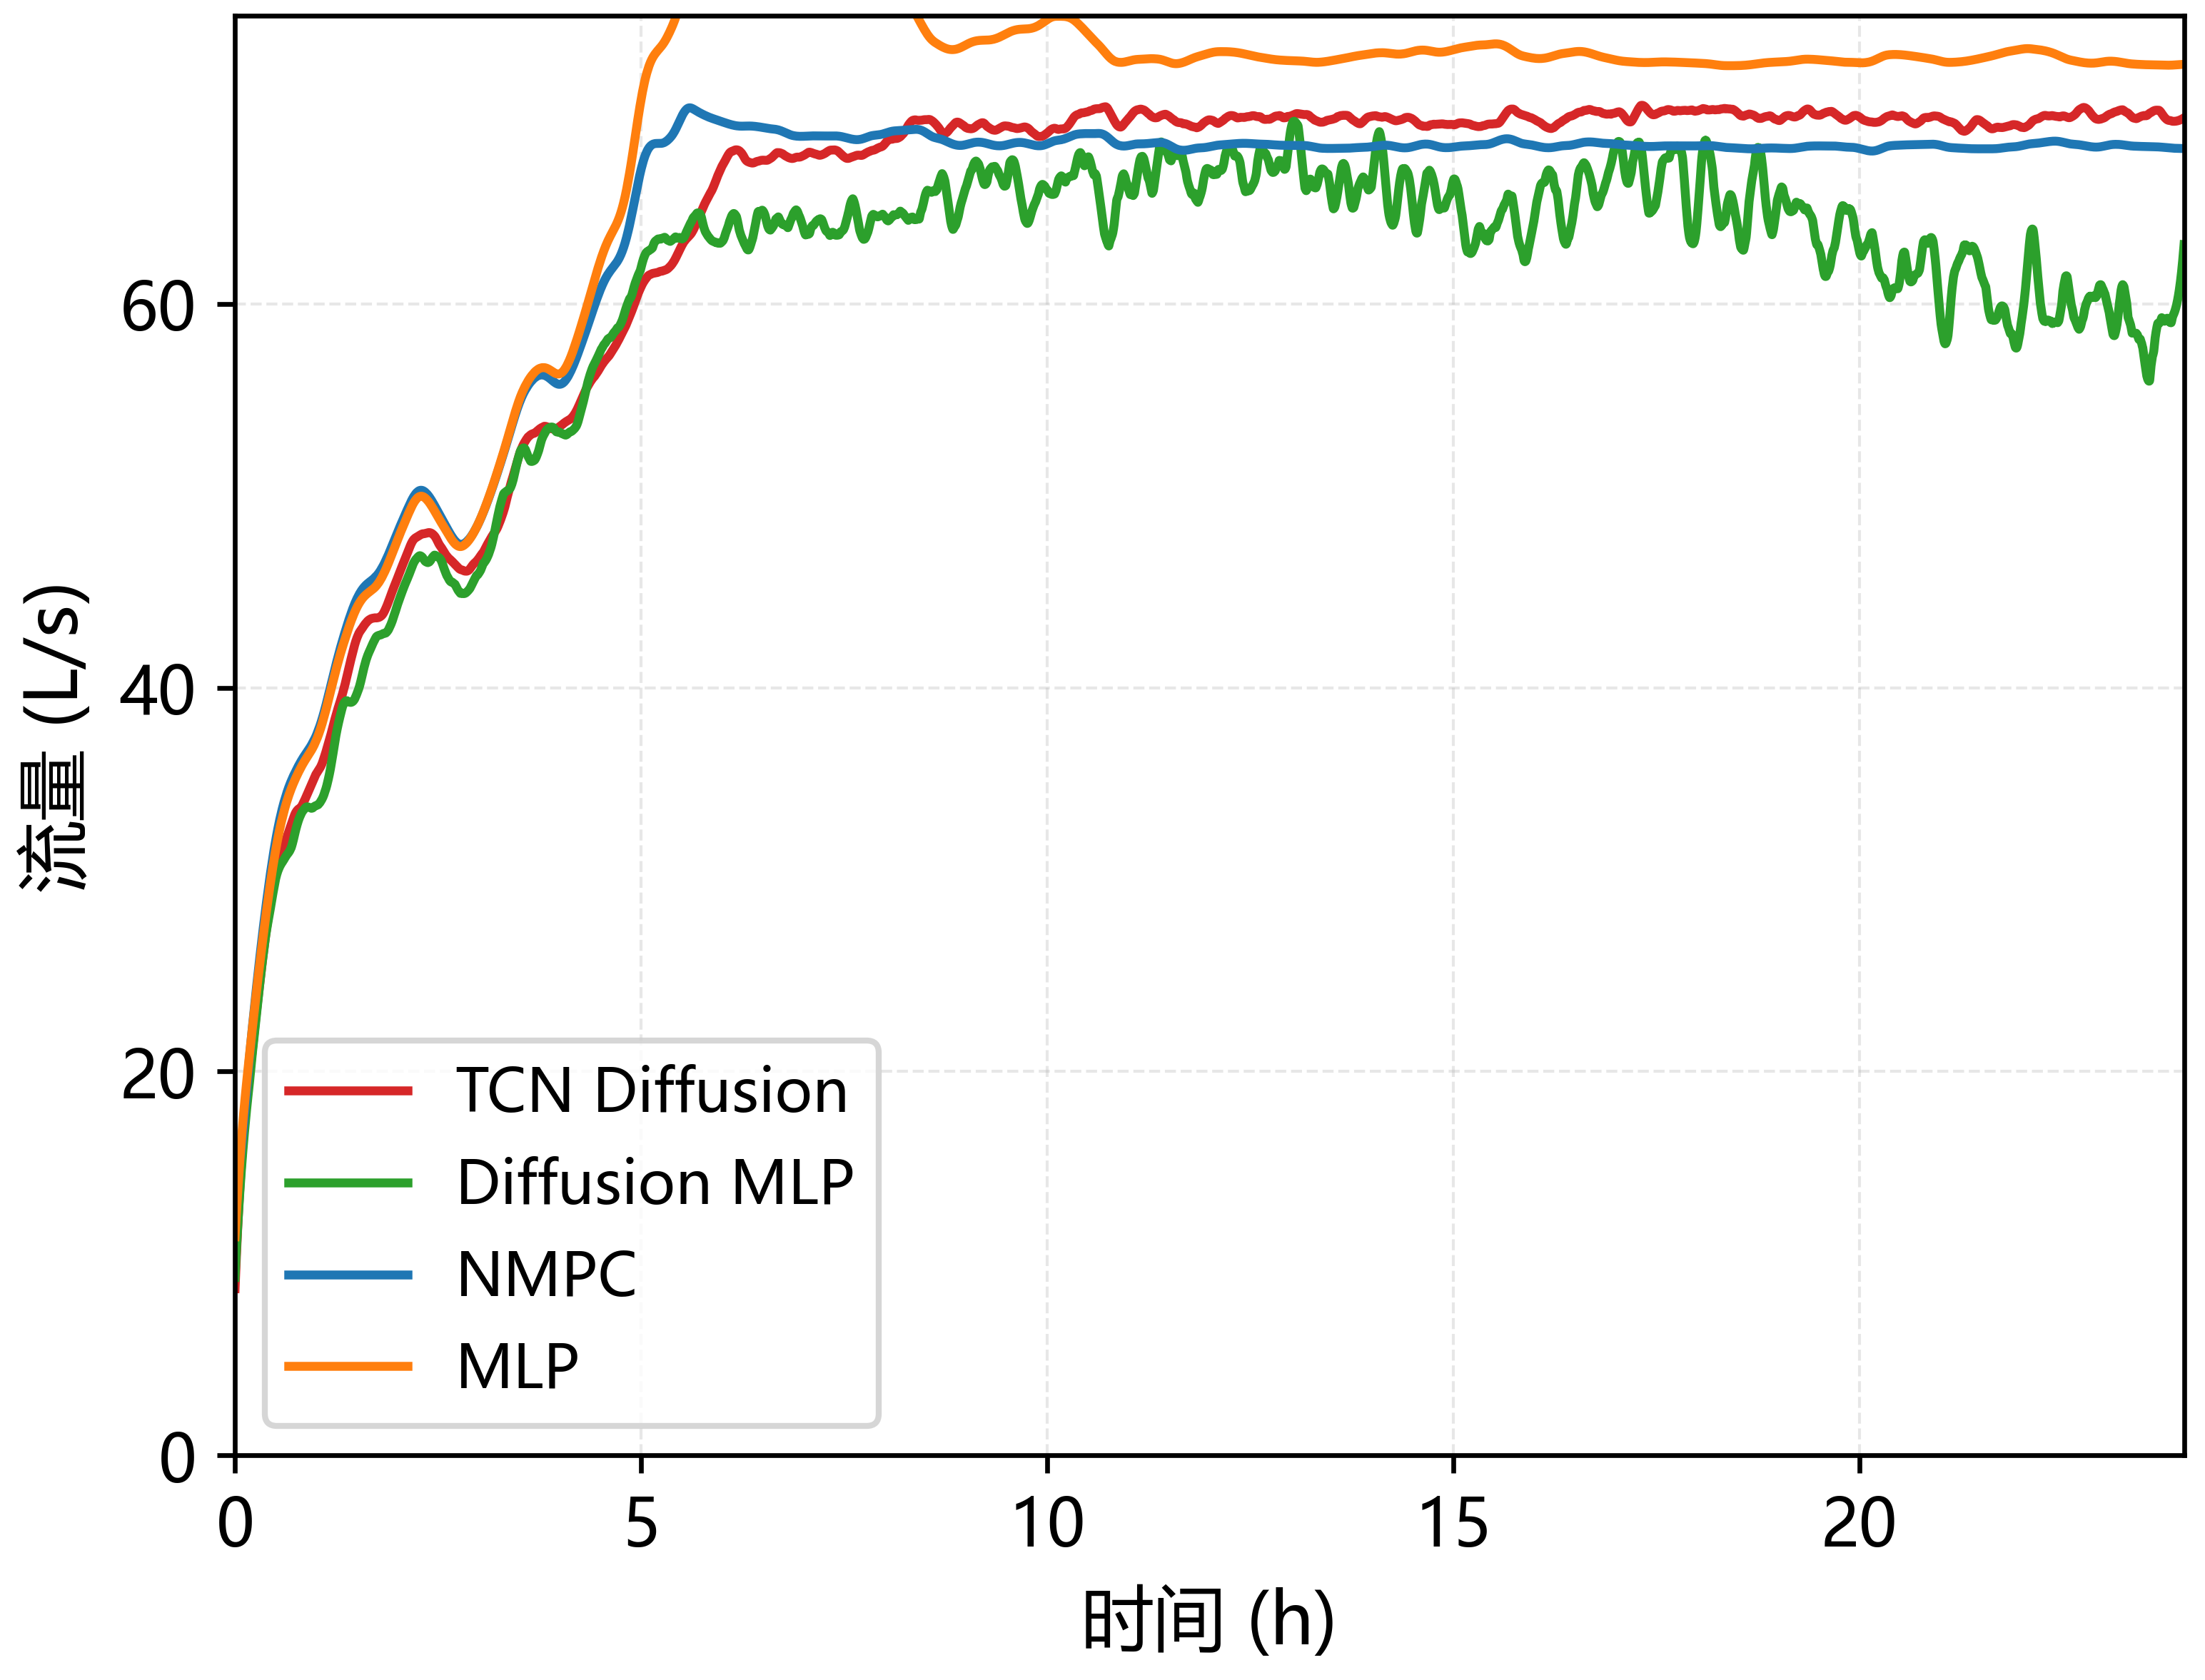
\includegraphics[width=\linewidth]{figures/controller_wind_comparison_f.png}
    \caption{}
  \end{subfigure}
  \caption{TCN Diffusion、Diffusion MLP、NMPC与MLP风电功率跟踪对比}
  \captionsetup{font=normalfont}
  \caption*{(a) 总功率跟踪；(b) 电解槽温度；(c) 氢氧杂质含量；(d) 电解槽电流；(e) 碱液流量；(f) 冷却水流量}
  \label{fig:controller_wind_comparison}
\end{figure}

% 上述实验检验了高动态波动场景，为进一步评估系统在低功率持续运行工况下的表现，补充了10月份风电功率曲线的24小时闭环仿真。如图~\ref{fig:controller_wind_oct_comparison}所示，10月份风电功率整体处于较低水平（8.00--10.78~MW，均值约8.33~MW），波动幅度远小于前文的剧烈波动场景，但持续低功率运行对系统的热平衡与气体分离动态提出了不同层面的挑战。在此场景下，Diffusion MLP的性能出现全面劣化：功率跟踪在低功率区间表现出明显滞后与过调，MAE骤升至1.597~MW；温度控制品质急剧恶化，MAE达4.940~K，峰值攀升至87.24$^\circ$C，已接近90$^\circ$C安全上限，表明MLP主干网络在低功率工况下对热动态的长期预测能力严重不足；HTO峰值升至1.44\%，安全裕度显著收窄；碱液流量波动极为剧烈（极差70.5~L/s），远超其他三种方法（12.0--13.3~L/s），大幅增加执行机构磨损与泵送能耗。相比之下，NMPC、TCN Diffusion与纯MLP在该场景下均保持稳定的控制品质：三者功率MAE均在0.11~MW以内，温度MAE在0.08--0.20~K之间，HTO峰值约1.06\%--1.07\%。纯MLP在此场景下的表现远优于Diffusion MLP，甚至接近NMPC，这一现象与阶跃工况中的较差表现形成鲜明对比，说明纯前馈网络在低功率平稳波动工况下具有良好的拟合能力，而扩散去噪过程与MLP主干的组合反而在低功率区间引入了对分布偏移的敏感性问题——训练数据中低功率样本相对稀疏，扩散去噪的迭代采样过程放大了MLP主干在该区域的预测偏差，导致性能劣化。

% \begin{figure}[!htbp]
%   \centering
%   \includegraphics[width=0.98\textwidth]{figures/controller_wind_oct_comparison.png}
%   \caption{TCN Diffusion、Diffusion MLP、NMPC与MLP 10月风电功率跟踪对比}
%   \label{fig:controller_wind_oct_comparison}
% \end{figure}

表~\ref{tab:wind_comparison} 汇总了四种方法在风电场景下的关键性能指标。在高动态场景中，四种方法的功率跟踪精度与HTO安全性相近，主要差异体现在控制量平滑性上。

\begin{table}[!htbp]
  \centering
  \caption{风电场景控制方法性能对比}
  \label{tab:wind_comparison}
  \begin{tabular}{@{}l c c c c@{}}
    \toprule
    \textbf{指标} & \textbf{NMPC} & \textbf{TCN Diffusion} & \textbf{Diffusion MLP} & \textbf{MLP} \\
    \midrule
    \multicolumn{5}{@{}l}{\textit{高动态风电场景}} \\
    功率RMSE (MW) & 6.101 & 6.103 & 6.098 & 6.108 \\
    功率MAE (MW) & 5.227 & 5.250 & 5.217 & 5.314 \\
    温度MAE (K) & 0.229 & 0.238 & 0.328 & 0.233 \\
    HTO峰值 (\%) & 0.87 & 0.87 & 0.87 & 0.87 \\
    碱液流量极差 (L/s) & 8.1 & 5.7 & 14.3 & 7.5 \\
    冷却水流量极差 (L/s) & 55.9 & 60.9 & 63.2 & 70.9 \\
    % \addlinespace
    % \multicolumn{5}{@{}l}{\textit{10月低功率风电场景}} \\
    % 功率RMSE (MW) & 0.162 & 0.170 & 1.758 & 0.172 \\
    % 功率MAE (MW) & 0.064 & 0.086 & 1.597 & 0.110 \\
    % 温度MAE (K) & 0.079 & 0.201 & 4.940 & 0.161 \\
    % HTO峰值 (\%) & 1.07 & 1.07 & 1.44 & 1.06 \\
    % 碱液流量极差 (L/s) & 12.0 & 13.3 & 70.5 & 12.2 \\
    % 冷却水流量极差 (L/s) & 5.3 & 6.7 & 6.5 & 5.1 \\
    \bottomrule
  \end{tabular}
\end{table}

% 综合两个风电场景可见：在风电功率剧烈波动的高动态场景中，四种方法的功率跟踪精度与HTO安全性相近，主要差异体现在控制量平滑性上。TCN Diffusion凭借时序卷积结构对历史动态的有效聚合，碱液与冷却水流量均最为平缓；Diffusion MLP因MLP主干缺乏时序记忆，碱液流量脉动最大；纯MLP的碱液调节尚可，但冷却水流量波动最广，反映出多变量协调能力不足；NMPC则通过在线优化保持较好的平滑性。纯MLP在高动态场景中的温度精度已接近NMPC，说明纯前馈网络对平稳波动的拟合能力尚可，但在阶跃突变工况中则表现出显著滞后，时序建模能力的缺失限制了其动态响应品质。而在低功率、小波动的持续运行场景中，Diffusion MLP因训练数据分布偏移问题导致性能全面劣化——功率跟踪滞后、温度逼近安全上限、HTO裕度收窄、碱液流量剧烈振荡；TCN Diffusion与纯MLP则始终保持稳定的控制品质，接近NMPC水平。这一对比表明：时序卷积结构对不同工况具有较强适应能力；纯前馈网络在平稳工况下可胜任，但对剧烈瞬态响应不足；扩散去噪机制虽能提升预测鲁棒性，但若与缺乏时序建模能力的主干网络结合，反而会在分布偏移区域放大预测偏差。

综合来看，在风电功率剧烈波动的高动态场景中，四种方法的功率跟踪精度与HTO安全性相近，主要差异体现在控制量平滑性上。TCN Diffusion凭借时序卷积结构对历史动态的有效聚合，碱液与冷却水流量均最为平缓；Diffusion MLP因MLP主干缺乏时序记忆，碱液流量脉动最大；纯MLP的碱液调节尚可，但冷却水流量波动最广，反映出多变量协调能力不足；NMPC则通过在线优化保持较好的平滑性。纯MLP在高动态场景中的温度精度已接近NMPC，说明纯前馈网络对平稳波动的拟合能力尚可，但在阶跃突变工况中则表现出显著滞后，时序建模能力的缺失限制了其动态响应品质。这一对比表明：时序卷积结构对不同工况具有较强适应能力；纯前馈网络在平稳工况下可胜任，但对剧烈瞬态响应不足；扩散去噪机制虽能提升预测鲁棒性，但若与缺乏时序建模能力的主干网络结合，反而会在分布偏移区域放大预测偏差。

\subsection{多重CBF联合约束闭环验证}

为验证3.4节所建立的多重CBF联合约束框架的实际控制效果，本节设计了两组典型工况实验：低功率HTO约束保护实验与高功率温度保护实验。前者检验系统在功率骤降工况下的HTO安全保持能力，后者检验系统在强产热工况下的温度上限约束能力。

\subsubsection{低功率HTO约束保护实验}

系统初始运行于3000~A稳态，$t=60$~min时刻参考电流阶跃降至1000~A，模拟可再生能源出力骤降。该工况下产气速率下降而气液分离动态滞后，阳极侧氢气累积导致HTO上升。CBF参数取$\gamma_{HTO}=1$、$\rho=5000$，与温度CBF联合构成多重约束体系。闭环验证结果如图~\ref{fig:cbf_hto_protection} 所示。

\begin{figure}[!htbp]
  \centering
  \begin{subfigure}{0.48\textwidth}
    \centering
    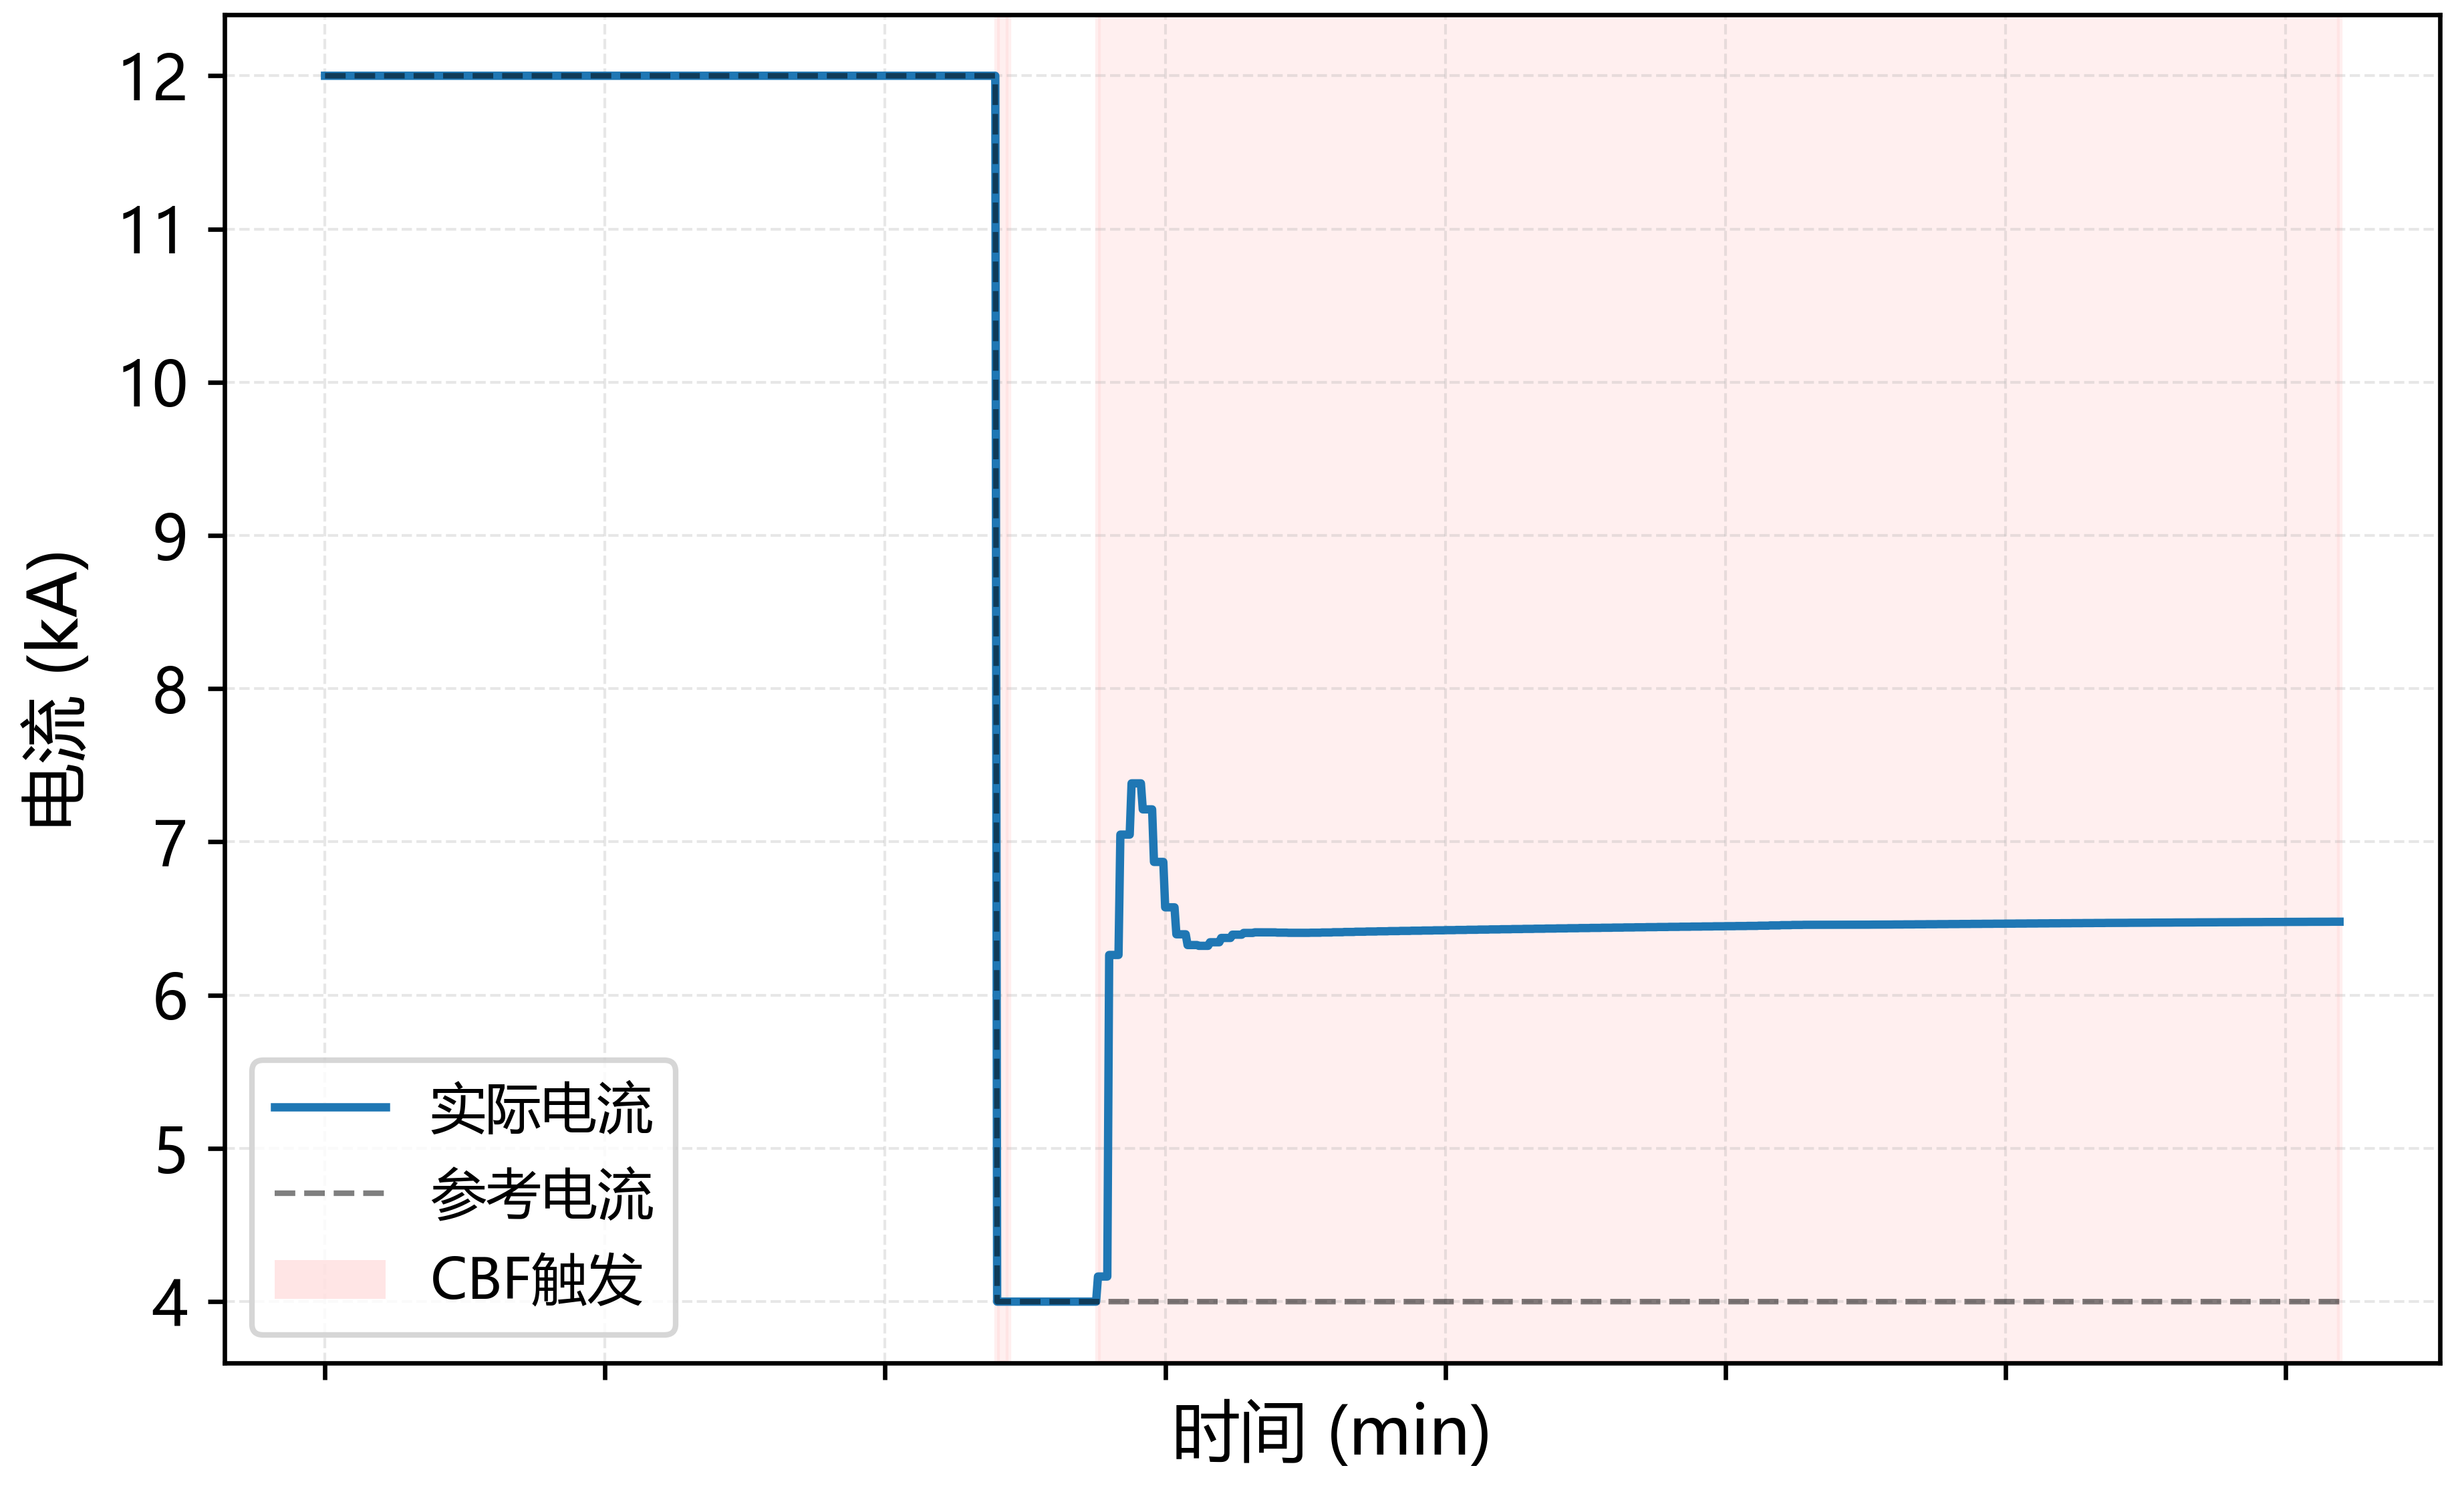
\includegraphics[width=\linewidth]{figures/cbf_hto_protection_a.png}
    \caption{}
  \end{subfigure}
  \hfill
  \begin{subfigure}{0.48\textwidth}
    \centering
    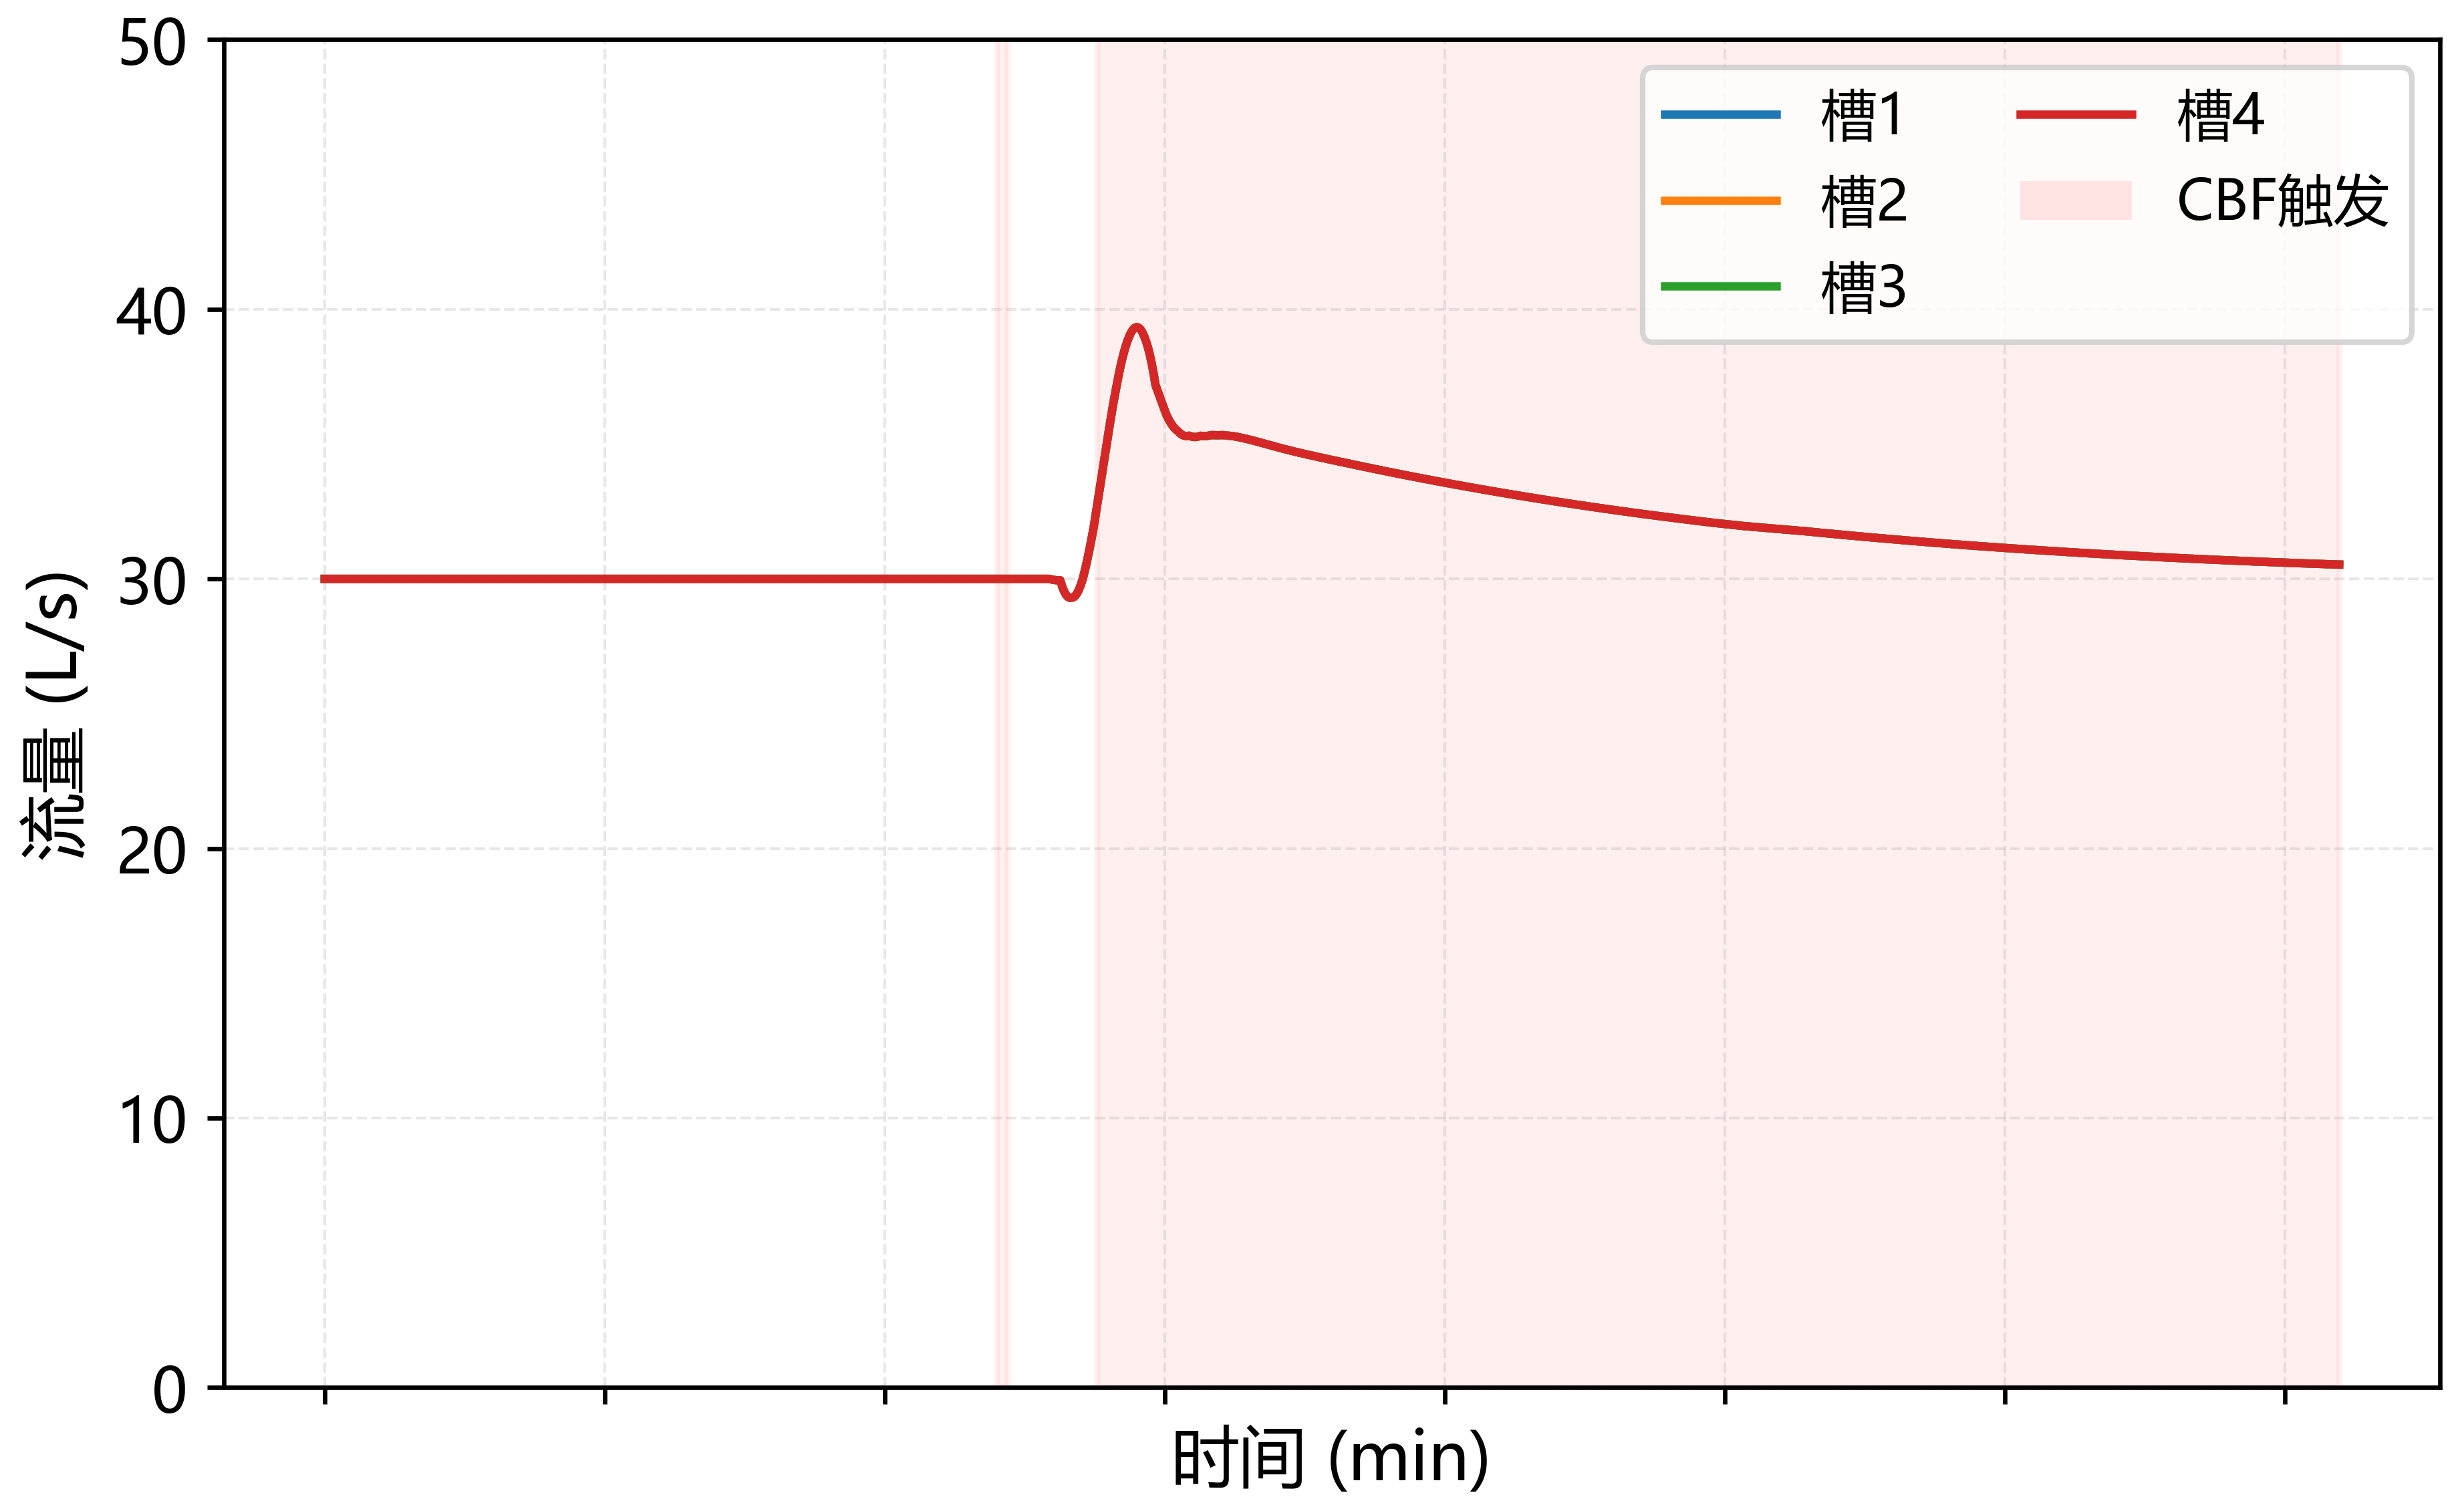
\includegraphics[width=\linewidth]{figures/cbf_hto_protection_b.png}
    \caption{}
  \end{subfigure}

  \begin{subfigure}{0.48\textwidth}
    \centering
    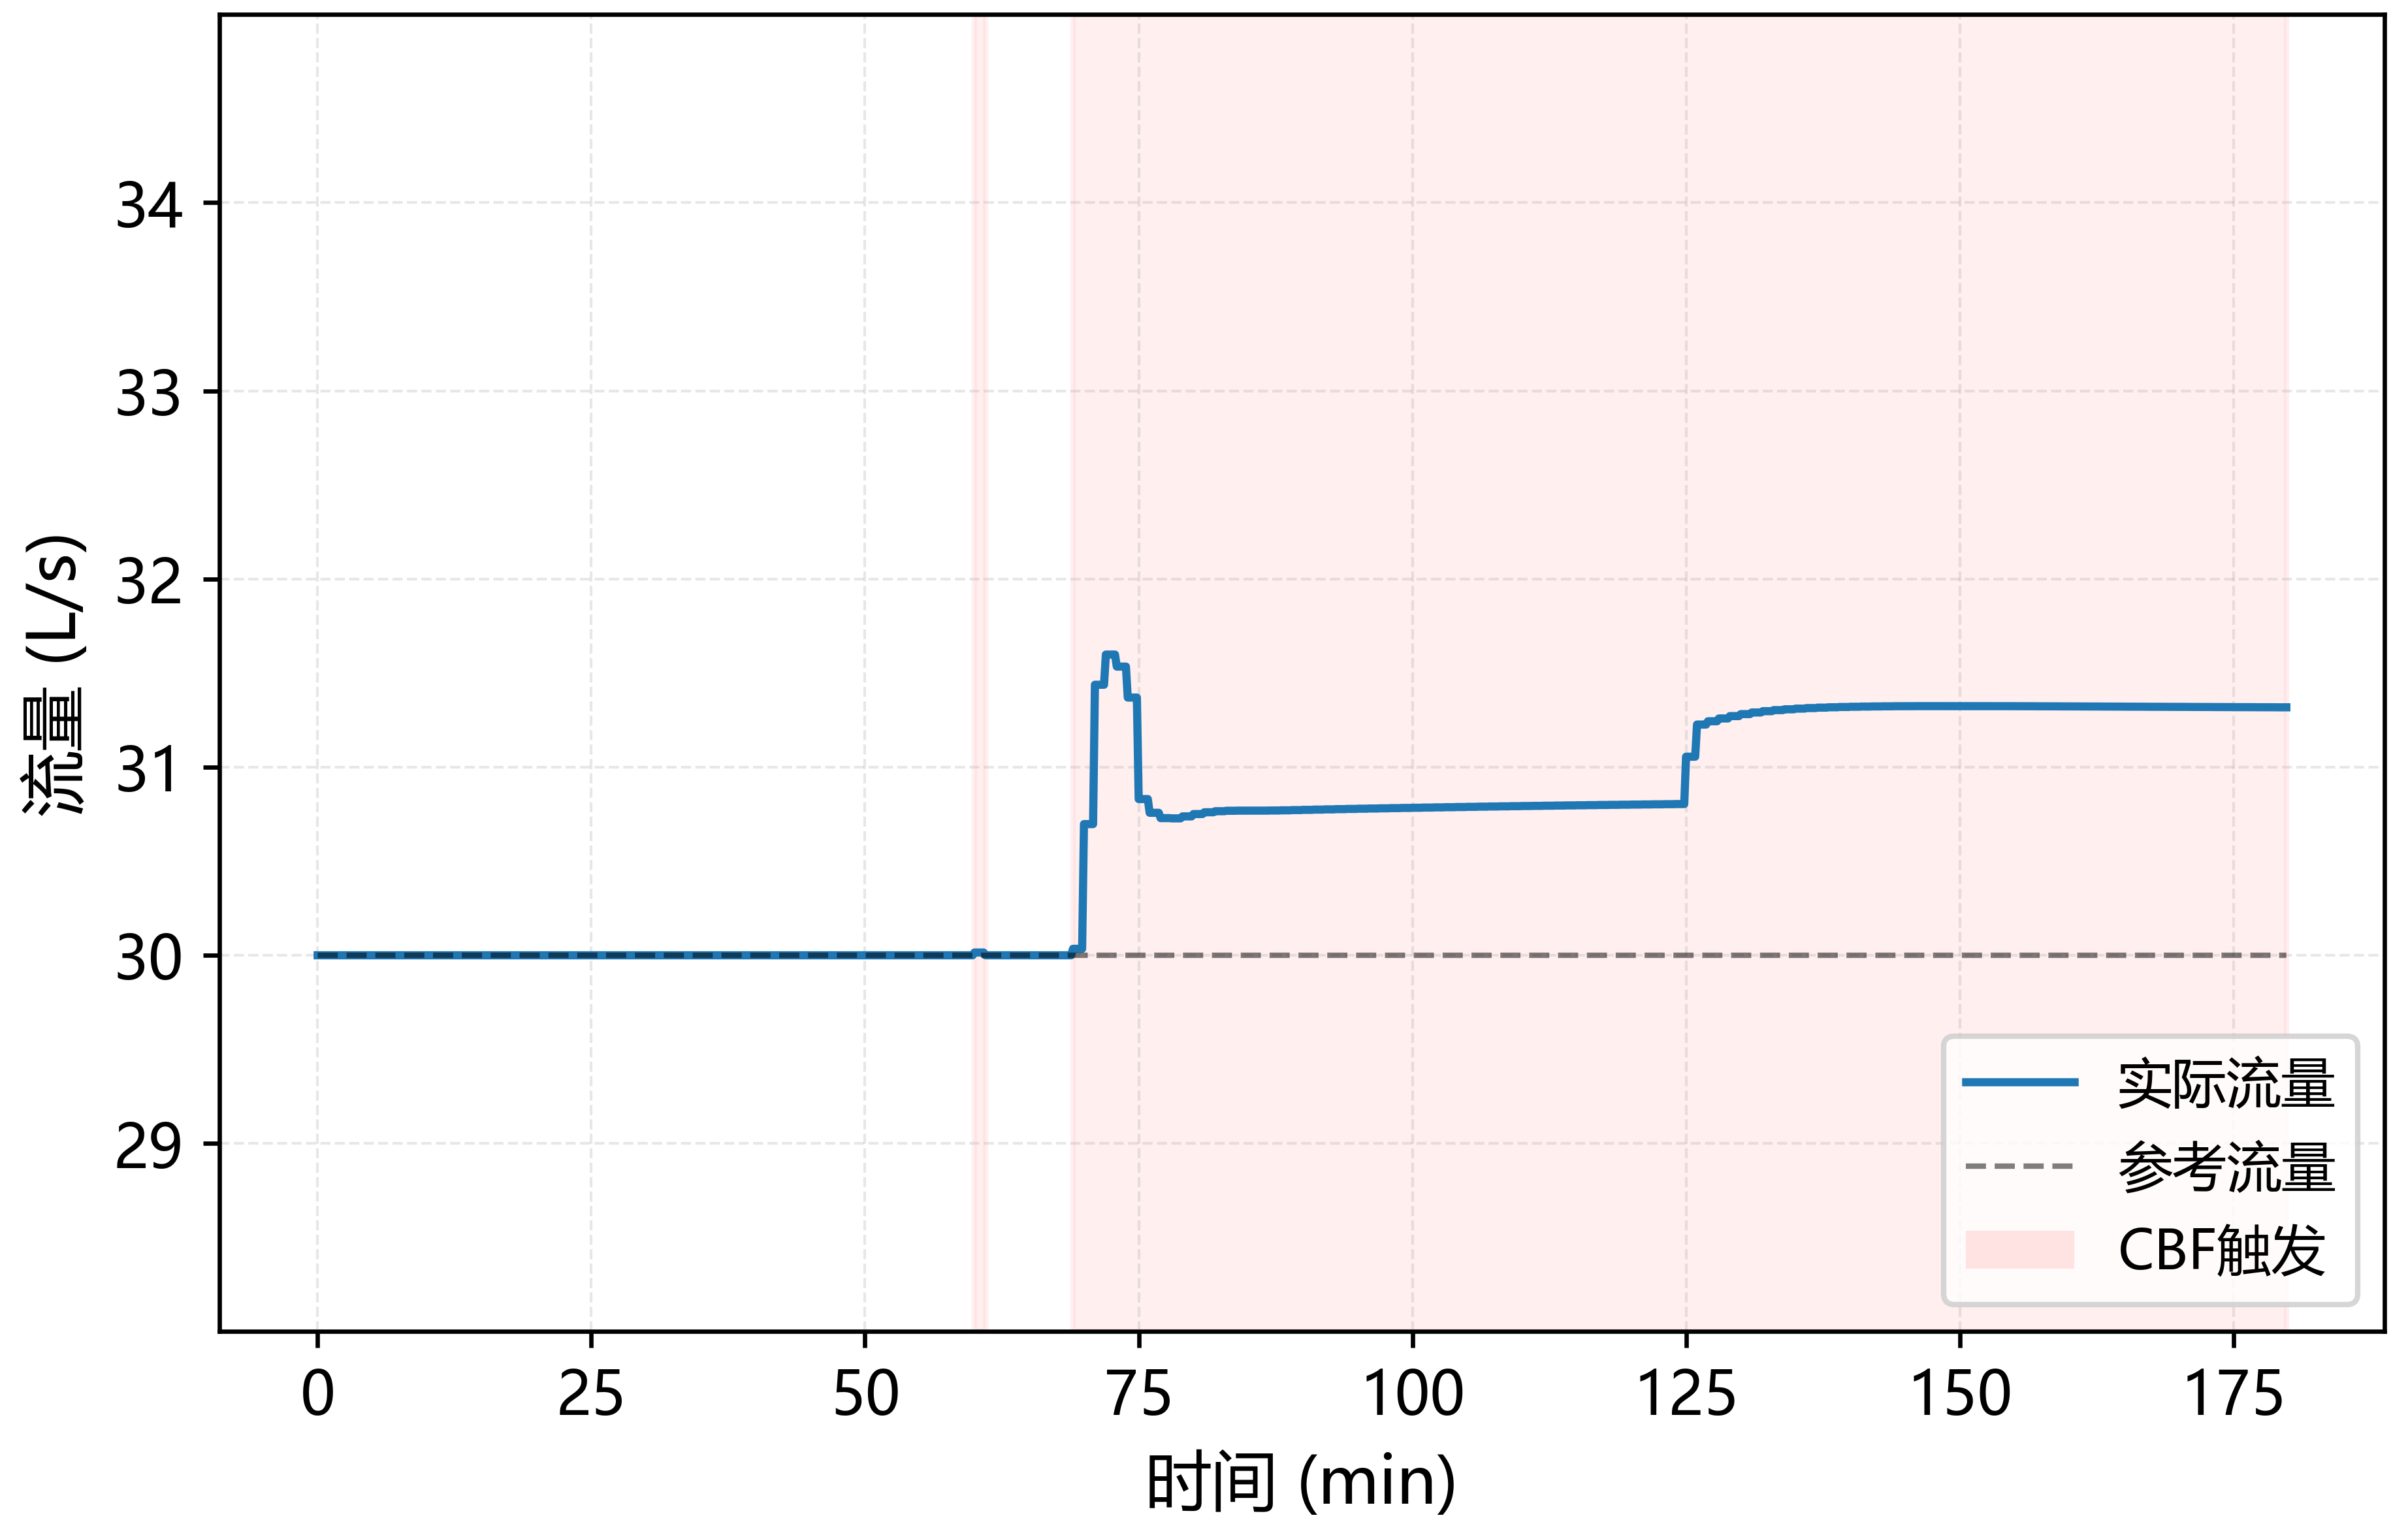
\includegraphics[width=\linewidth]{figures/cbf_hto_protection_c.png}
    \caption{}
  \end{subfigure}
  \hfill
  \begin{subfigure}{0.48\textwidth}
    \centering
    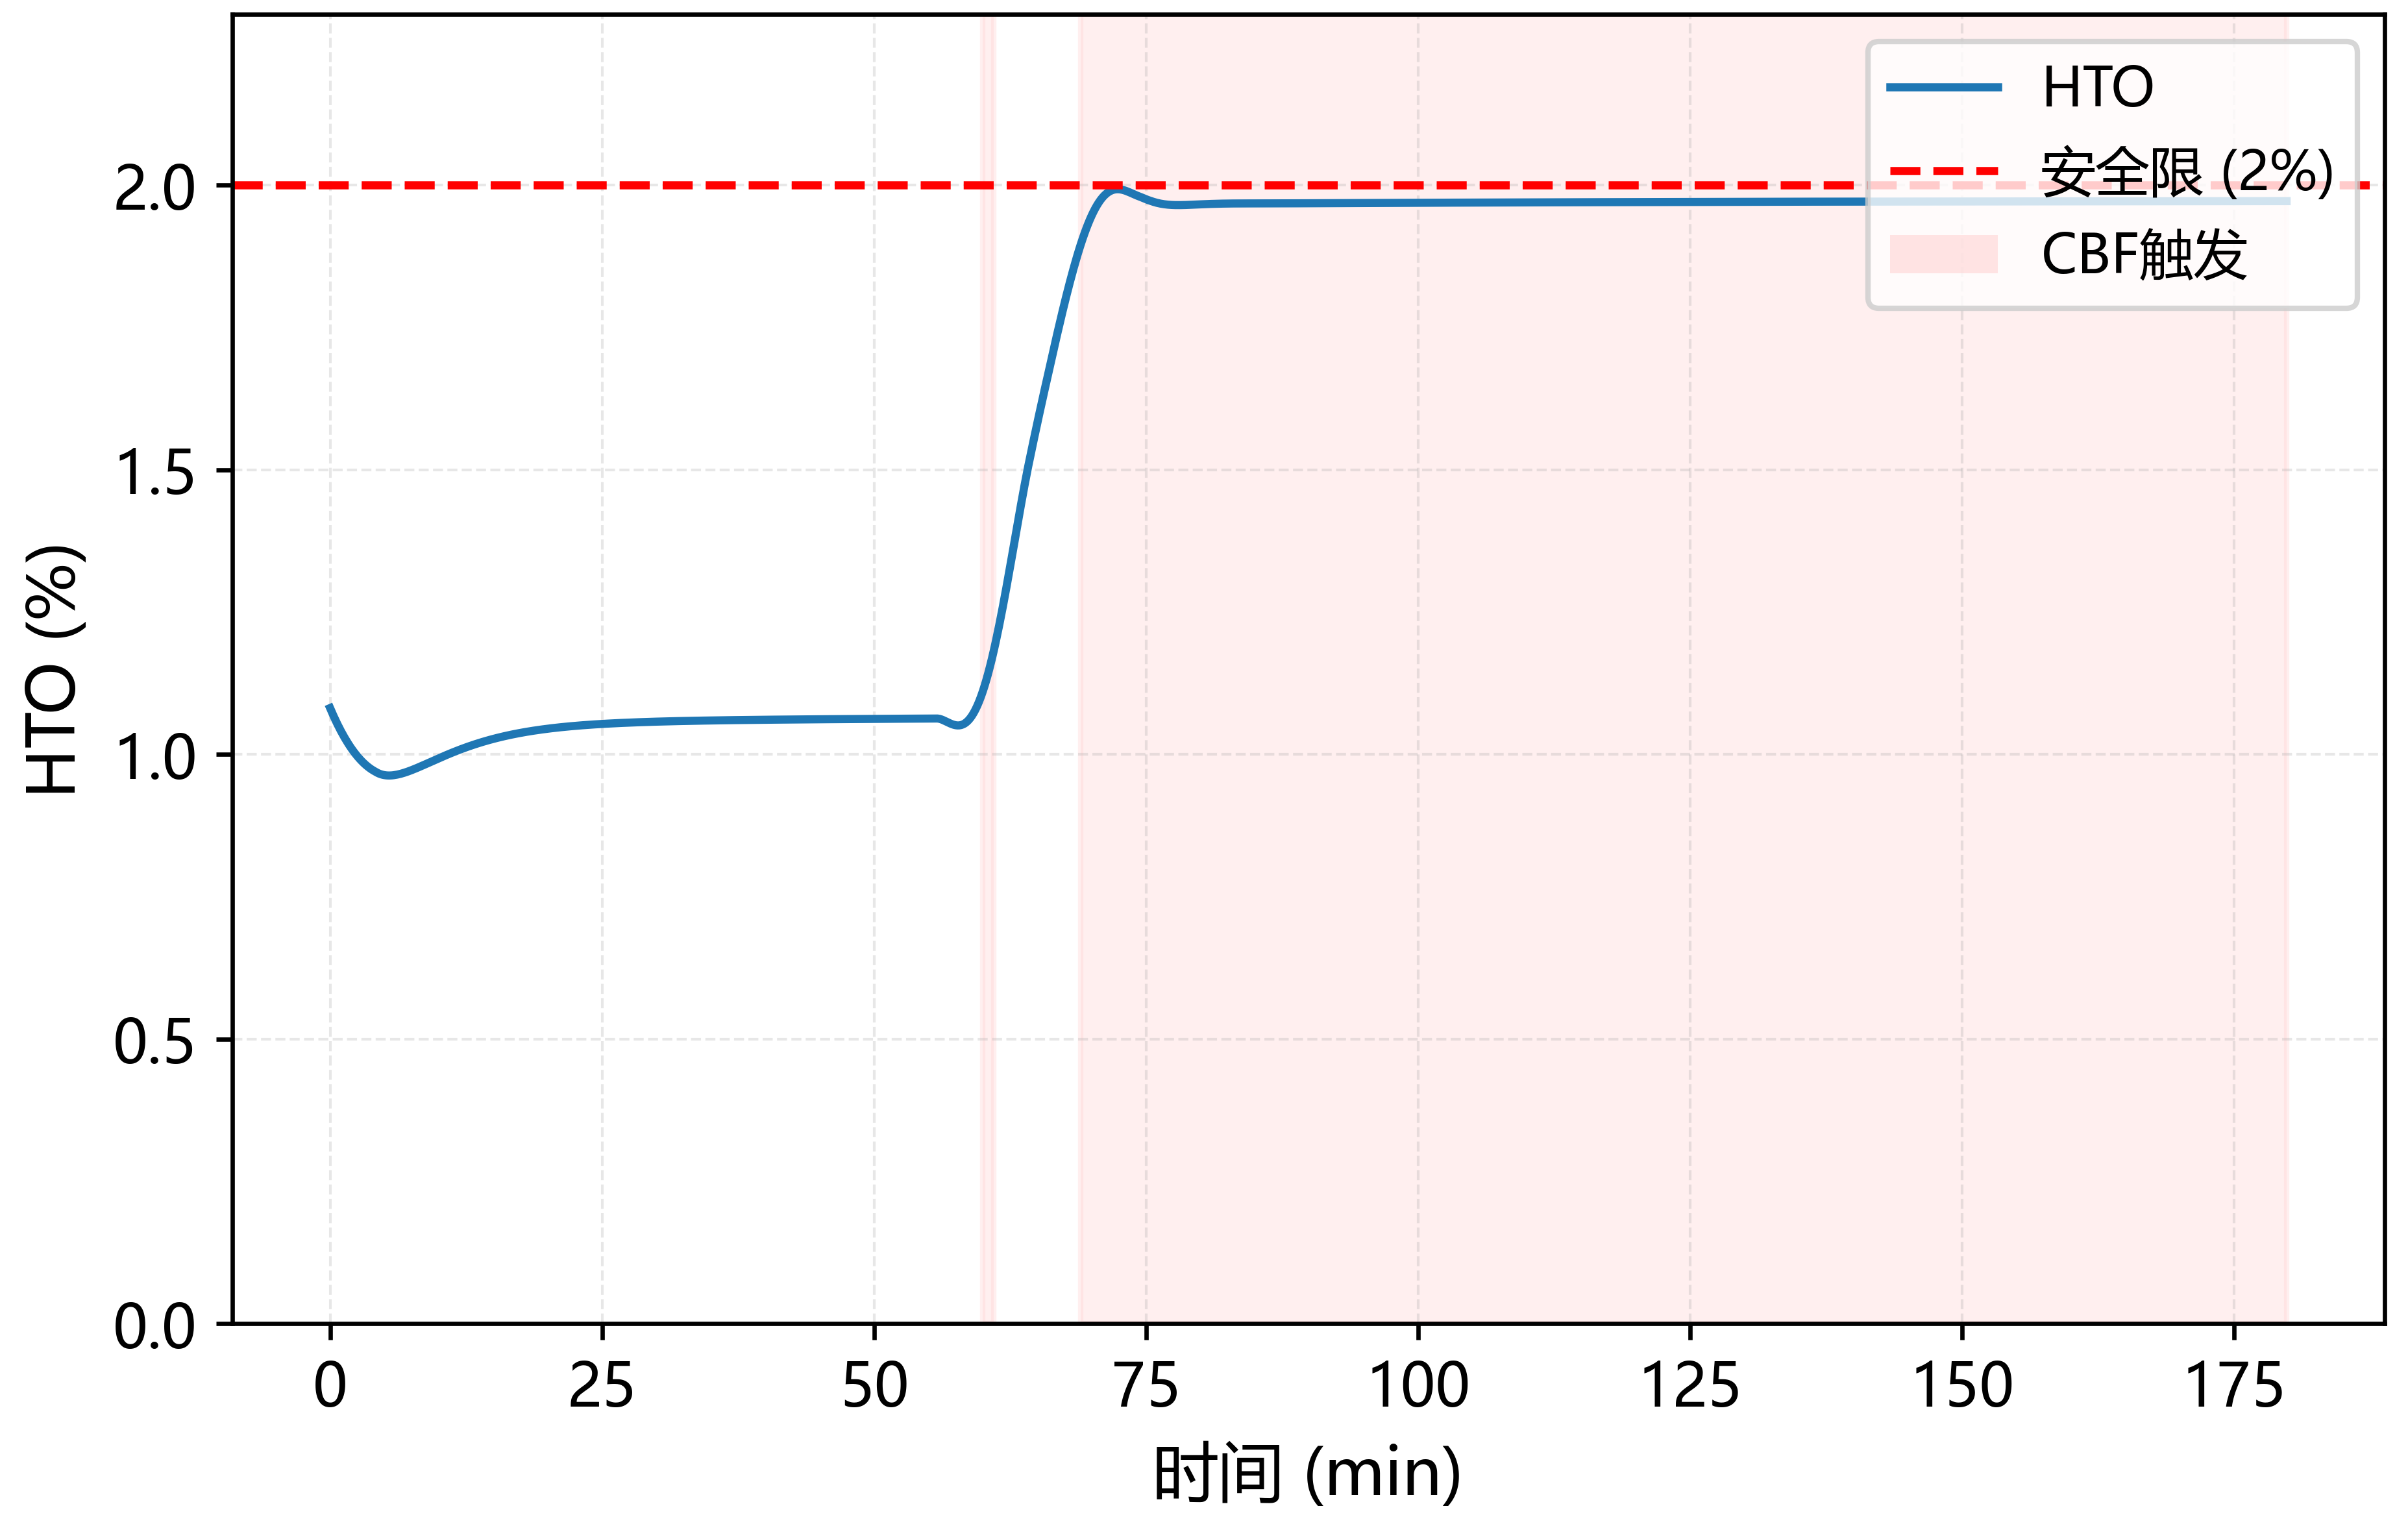
\includegraphics[width=\linewidth]{figures/cbf_hto_protection_d.png}
    \caption{}
  \end{subfigure}
  \caption{多重CBF联合约束闭环验证结果（HTO约束保护工况）}
  \captionsetup{font=normalfont}
  \caption*{(a) 电解槽电流；(b) 碱液流量；(c) 冷却水流量；(d) HTO安全控制}
  \label{fig:cbf_hto_protection}
\end{figure}

图~\ref{fig:cbf_hto_protection} 中HTO子图顶部红色指示条标记了CBF触发时刻。尽管动态滞后导致HTO呈上升趋势，CBF安全滤波通过及时增大碱液流量并适度调节电流，将HTO严格抑制在2\%安全阈值以下（峰值1.99\%）。这一控制分配与式~\eqref{eq:h_hto_expanded} 的物理结构一致：碱液流量以仿射形式直接作用于$\dot{h}_{HTO}$，调节灵敏度最高，故CBF优先通过增大流量快速抑制氢气累积；电流则以非仿射耦合项$\gamma(\mathbf{x}) \cdot u_1 \cdot \eta_F$进入约束，受法拉第效率饱和特性制约，其边际改善有限且伴随功率损失，因此仅被适度调节。一阶CBF通过合理设置$\gamma_{HTO}$与松弛惩罚系数$\rho$，在确保HTO不越界的同时实现了控制量的平滑过渡，验证了本节所建立的CBF安全滤波框架在低功率HTO约束保护工况下的有效性。
\begin{figure}[!htbp]
  \centering
  \begin{subfigure}{0.48\textwidth}
    \centering
    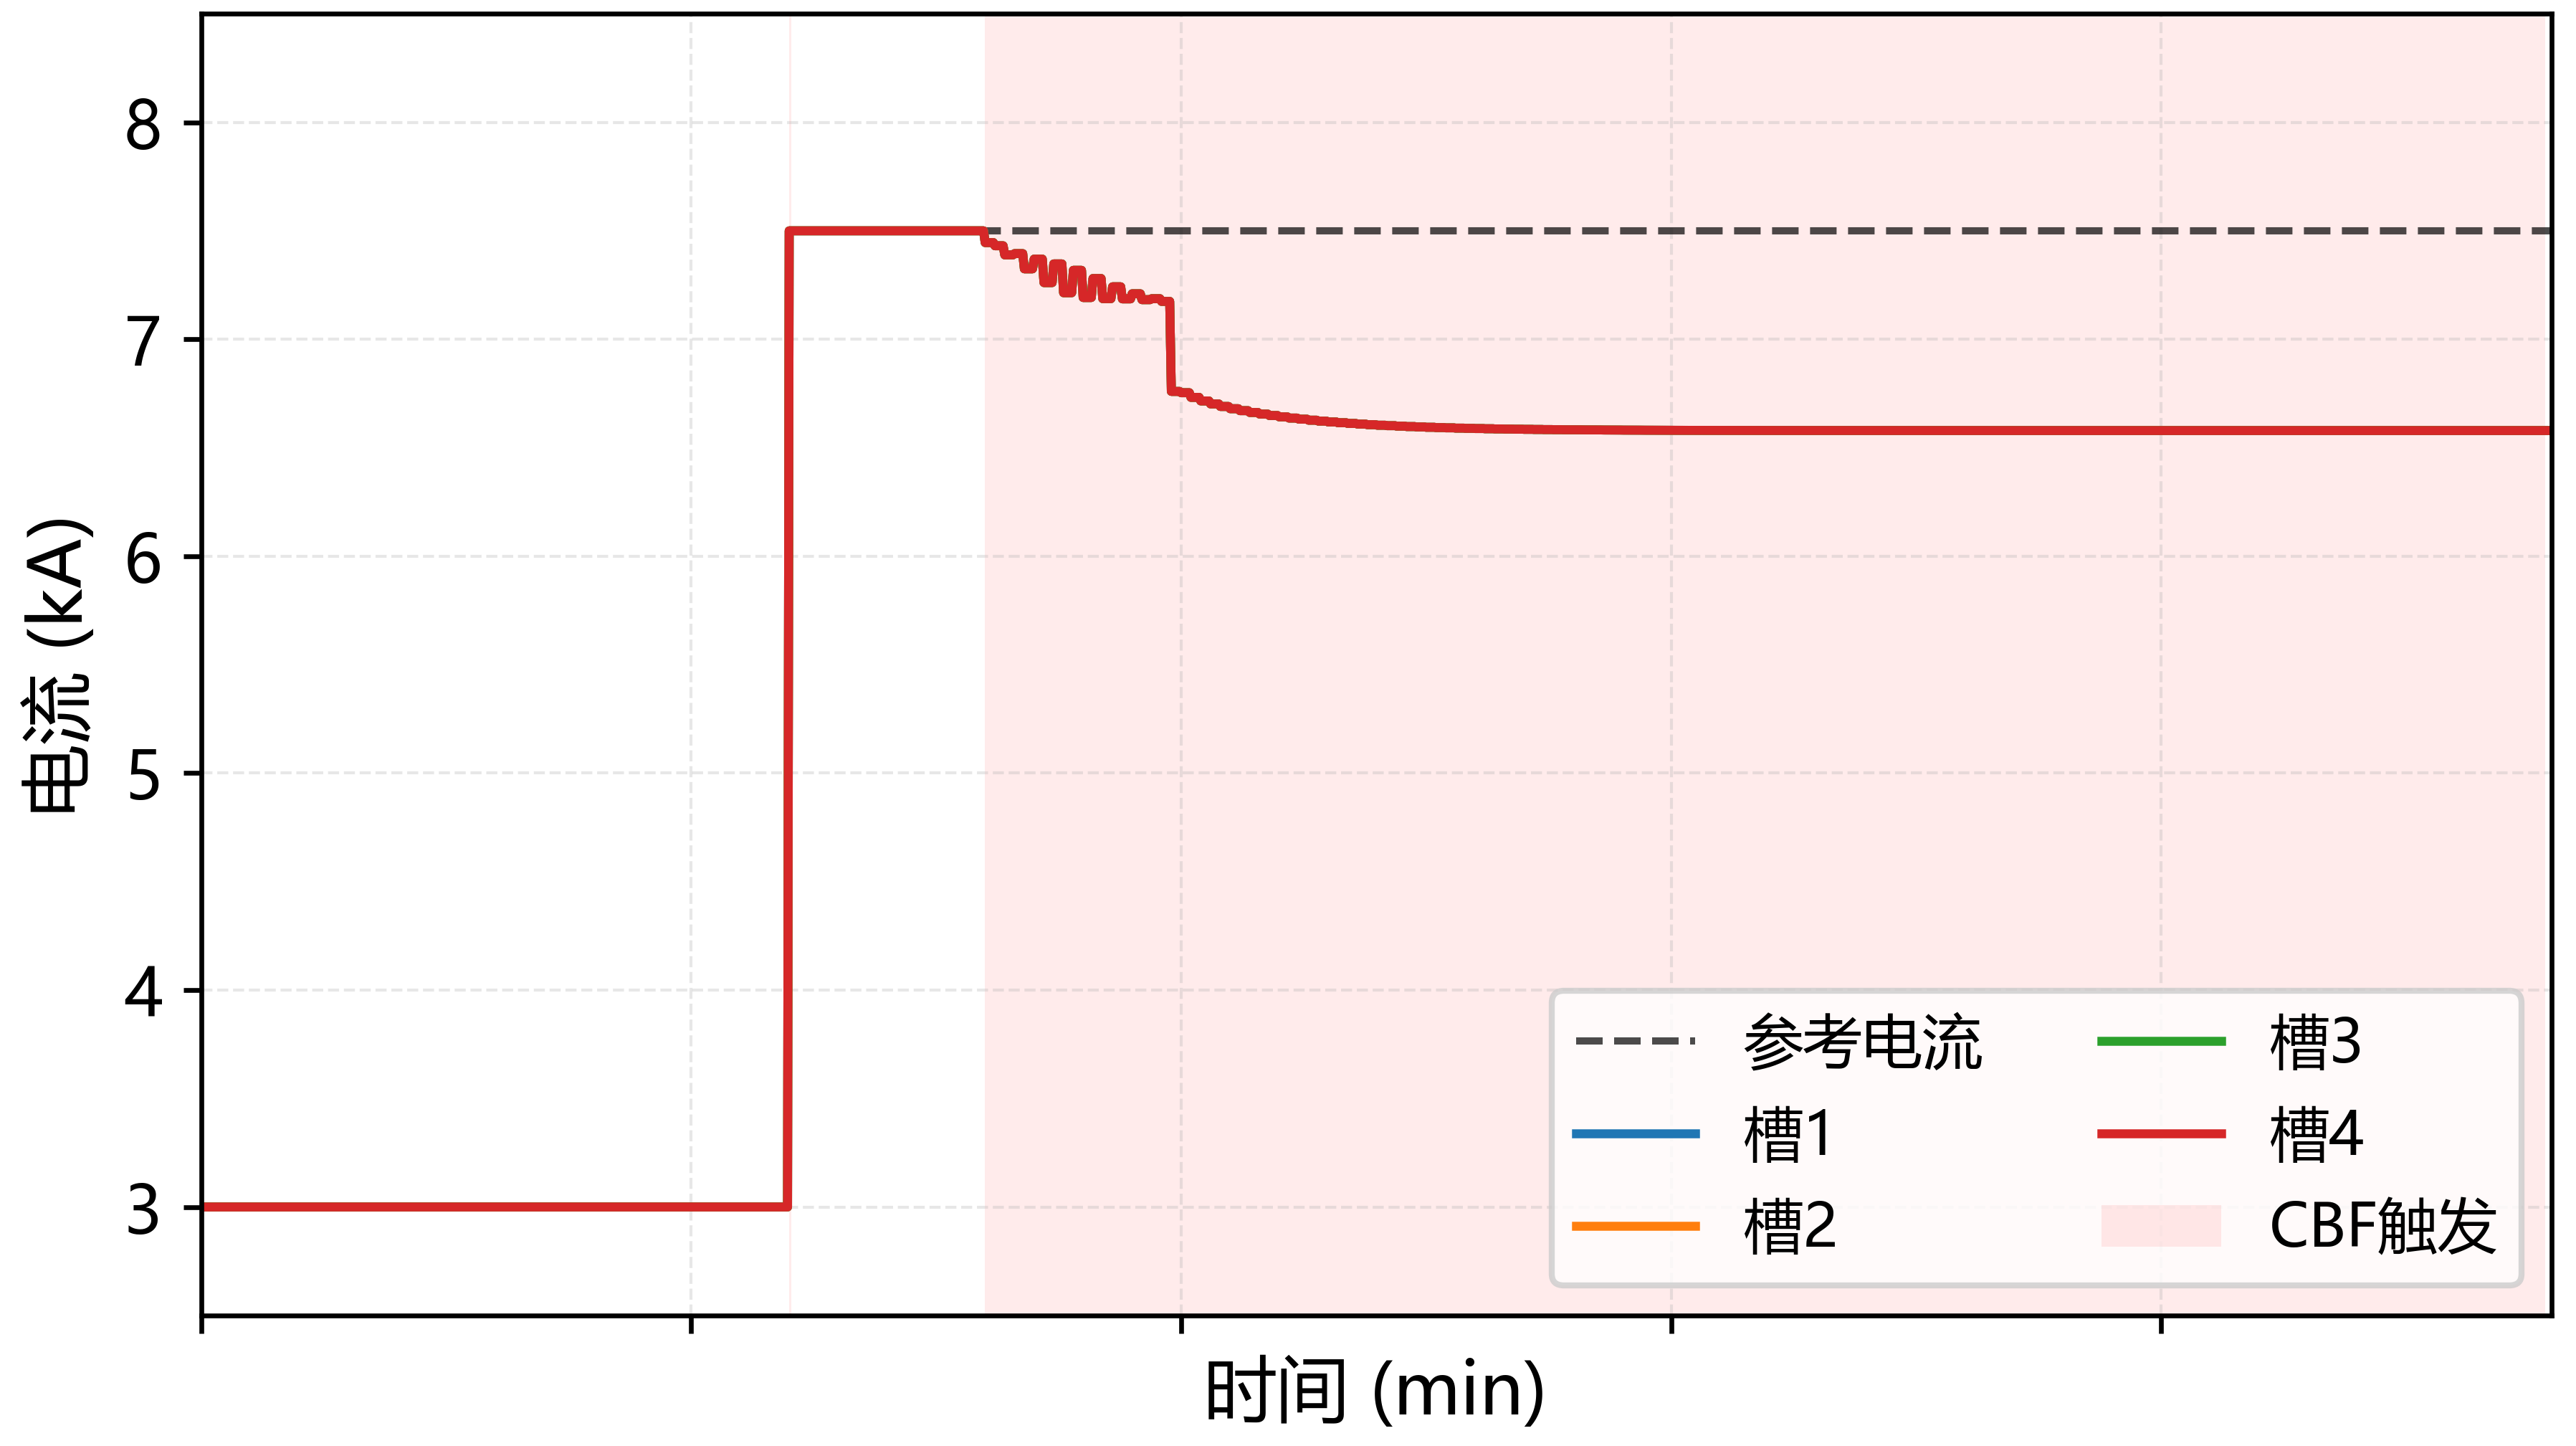
\includegraphics[width=\linewidth]{figures/cbf_temp_protection_a.png}
    \caption{}
  \end{subfigure}
  \hfill
  \begin{subfigure}{0.48\textwidth}
    \centering
    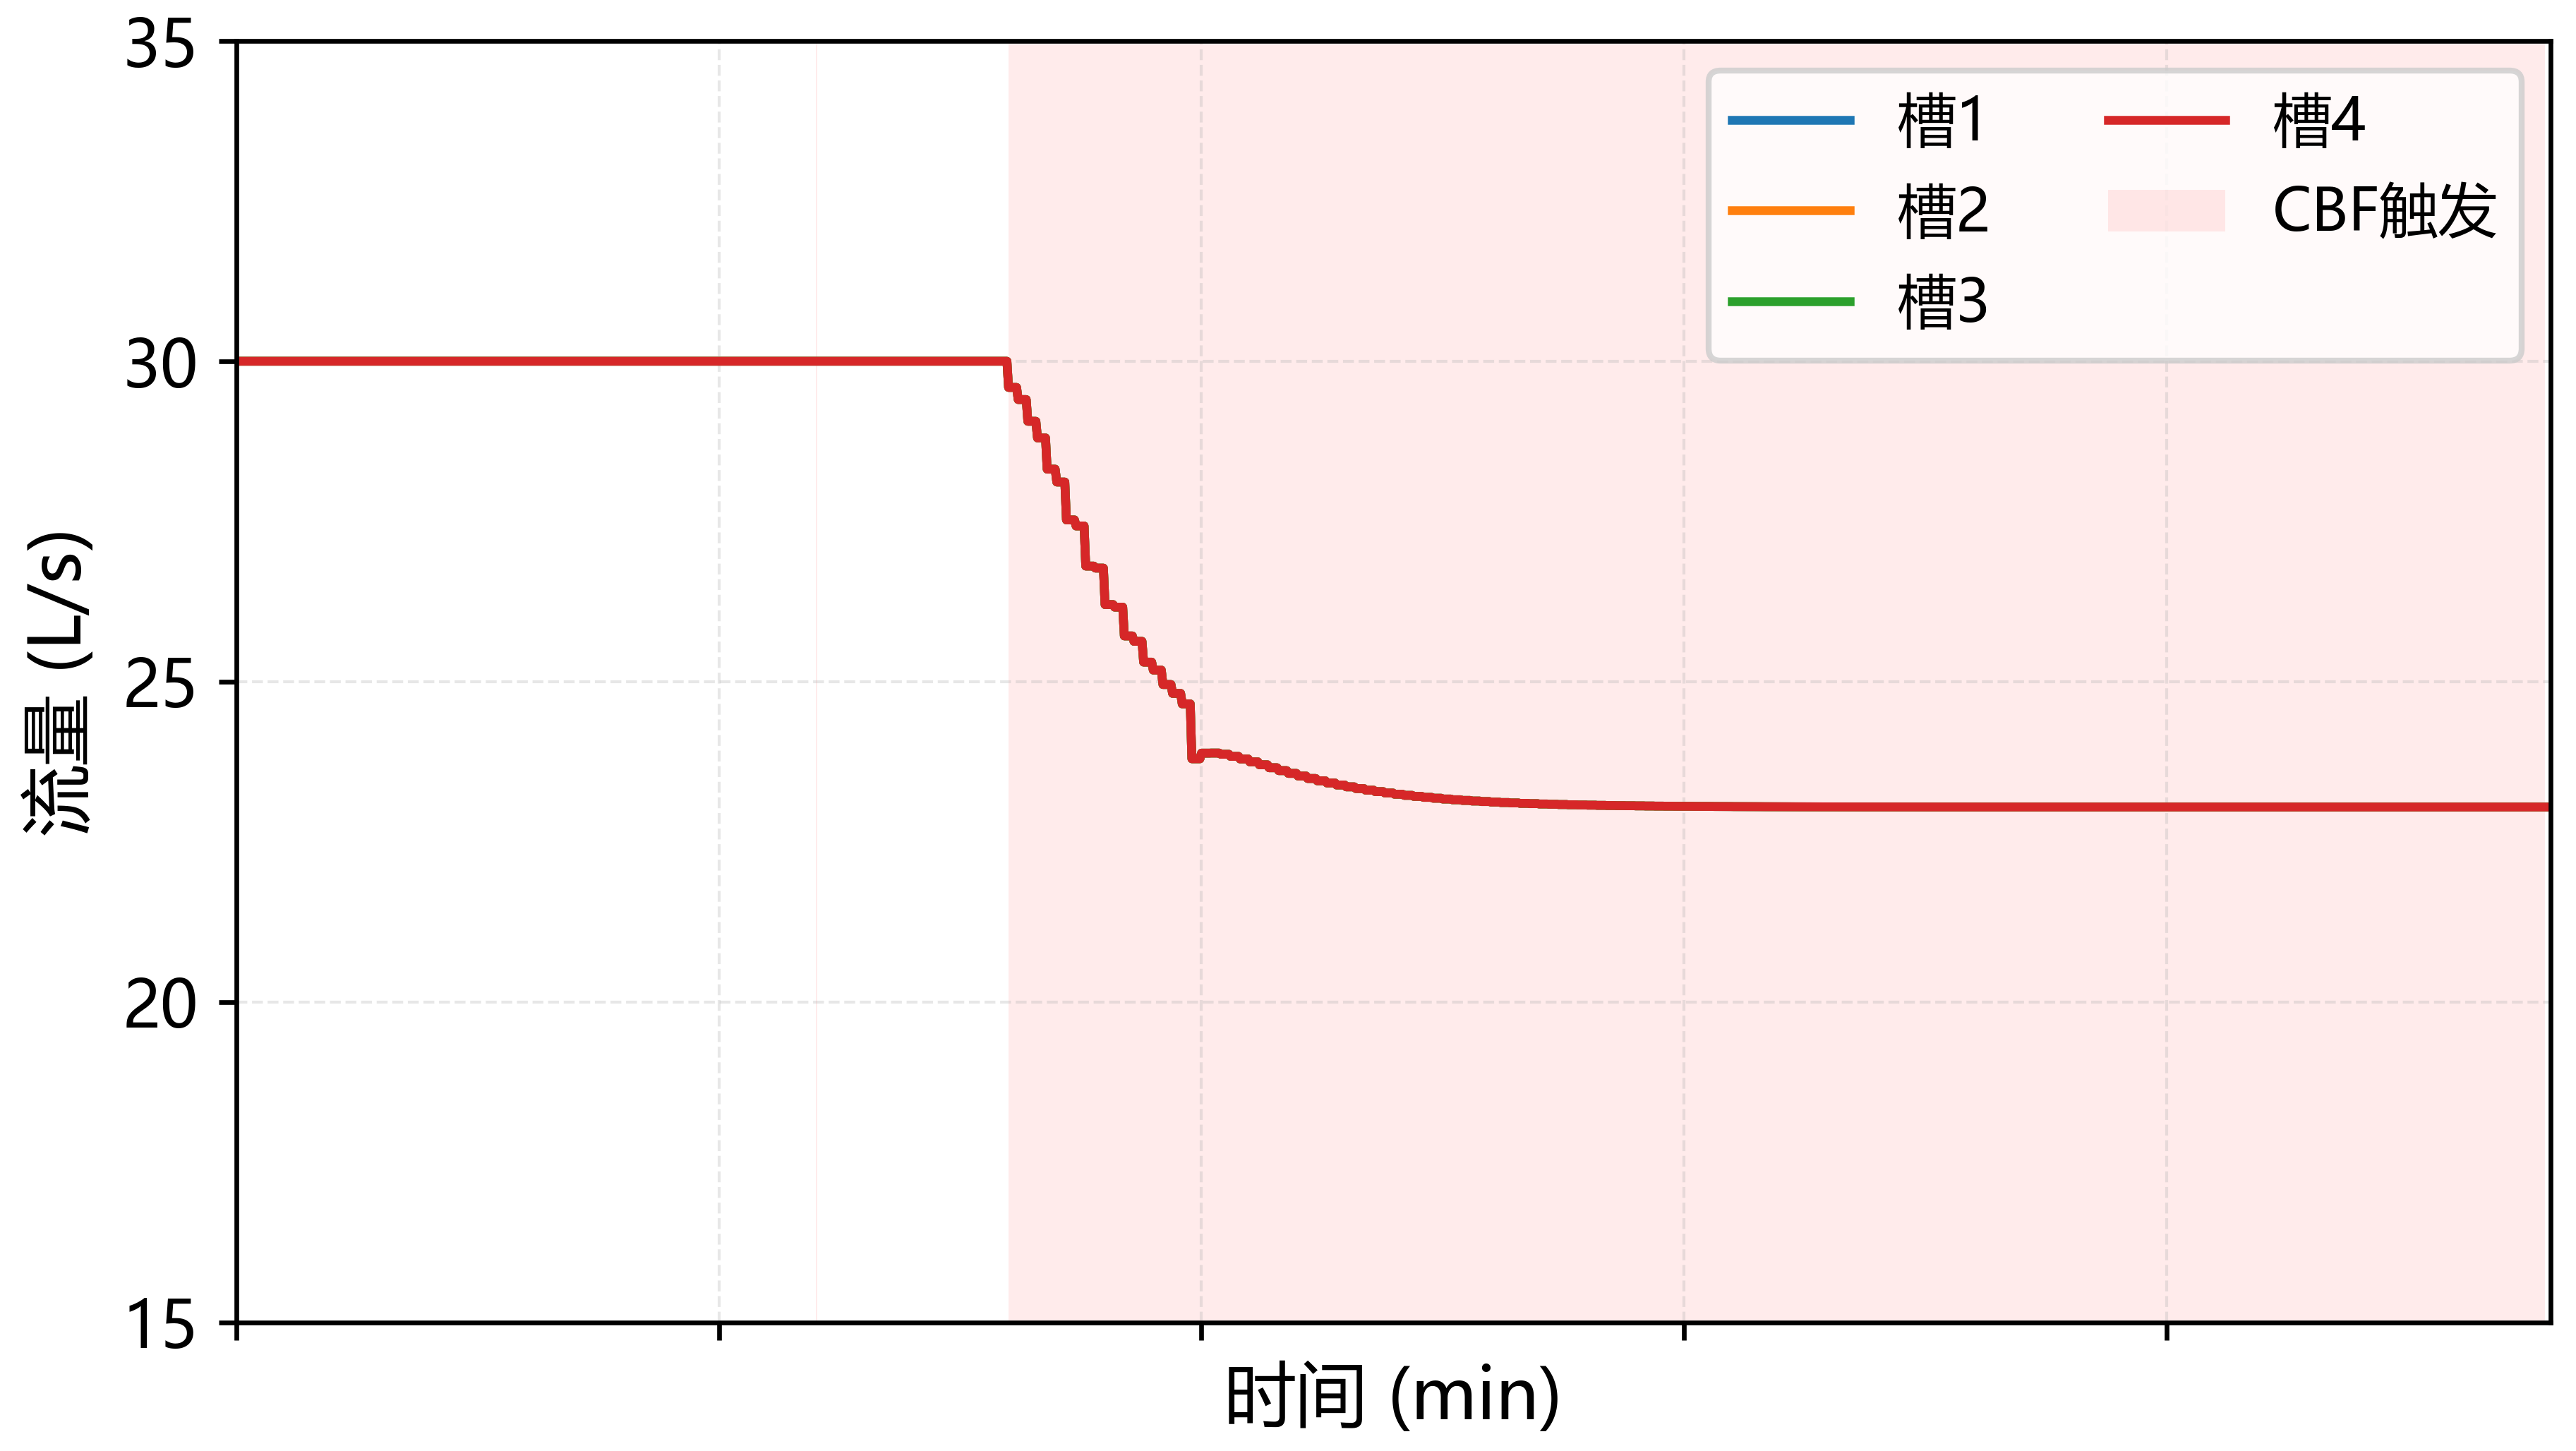
\includegraphics[width=\linewidth]{figures/cbf_temp_protection_b.png}
    \caption{}
  \end{subfigure}

  \begin{subfigure}{0.48\textwidth}
    \centering
    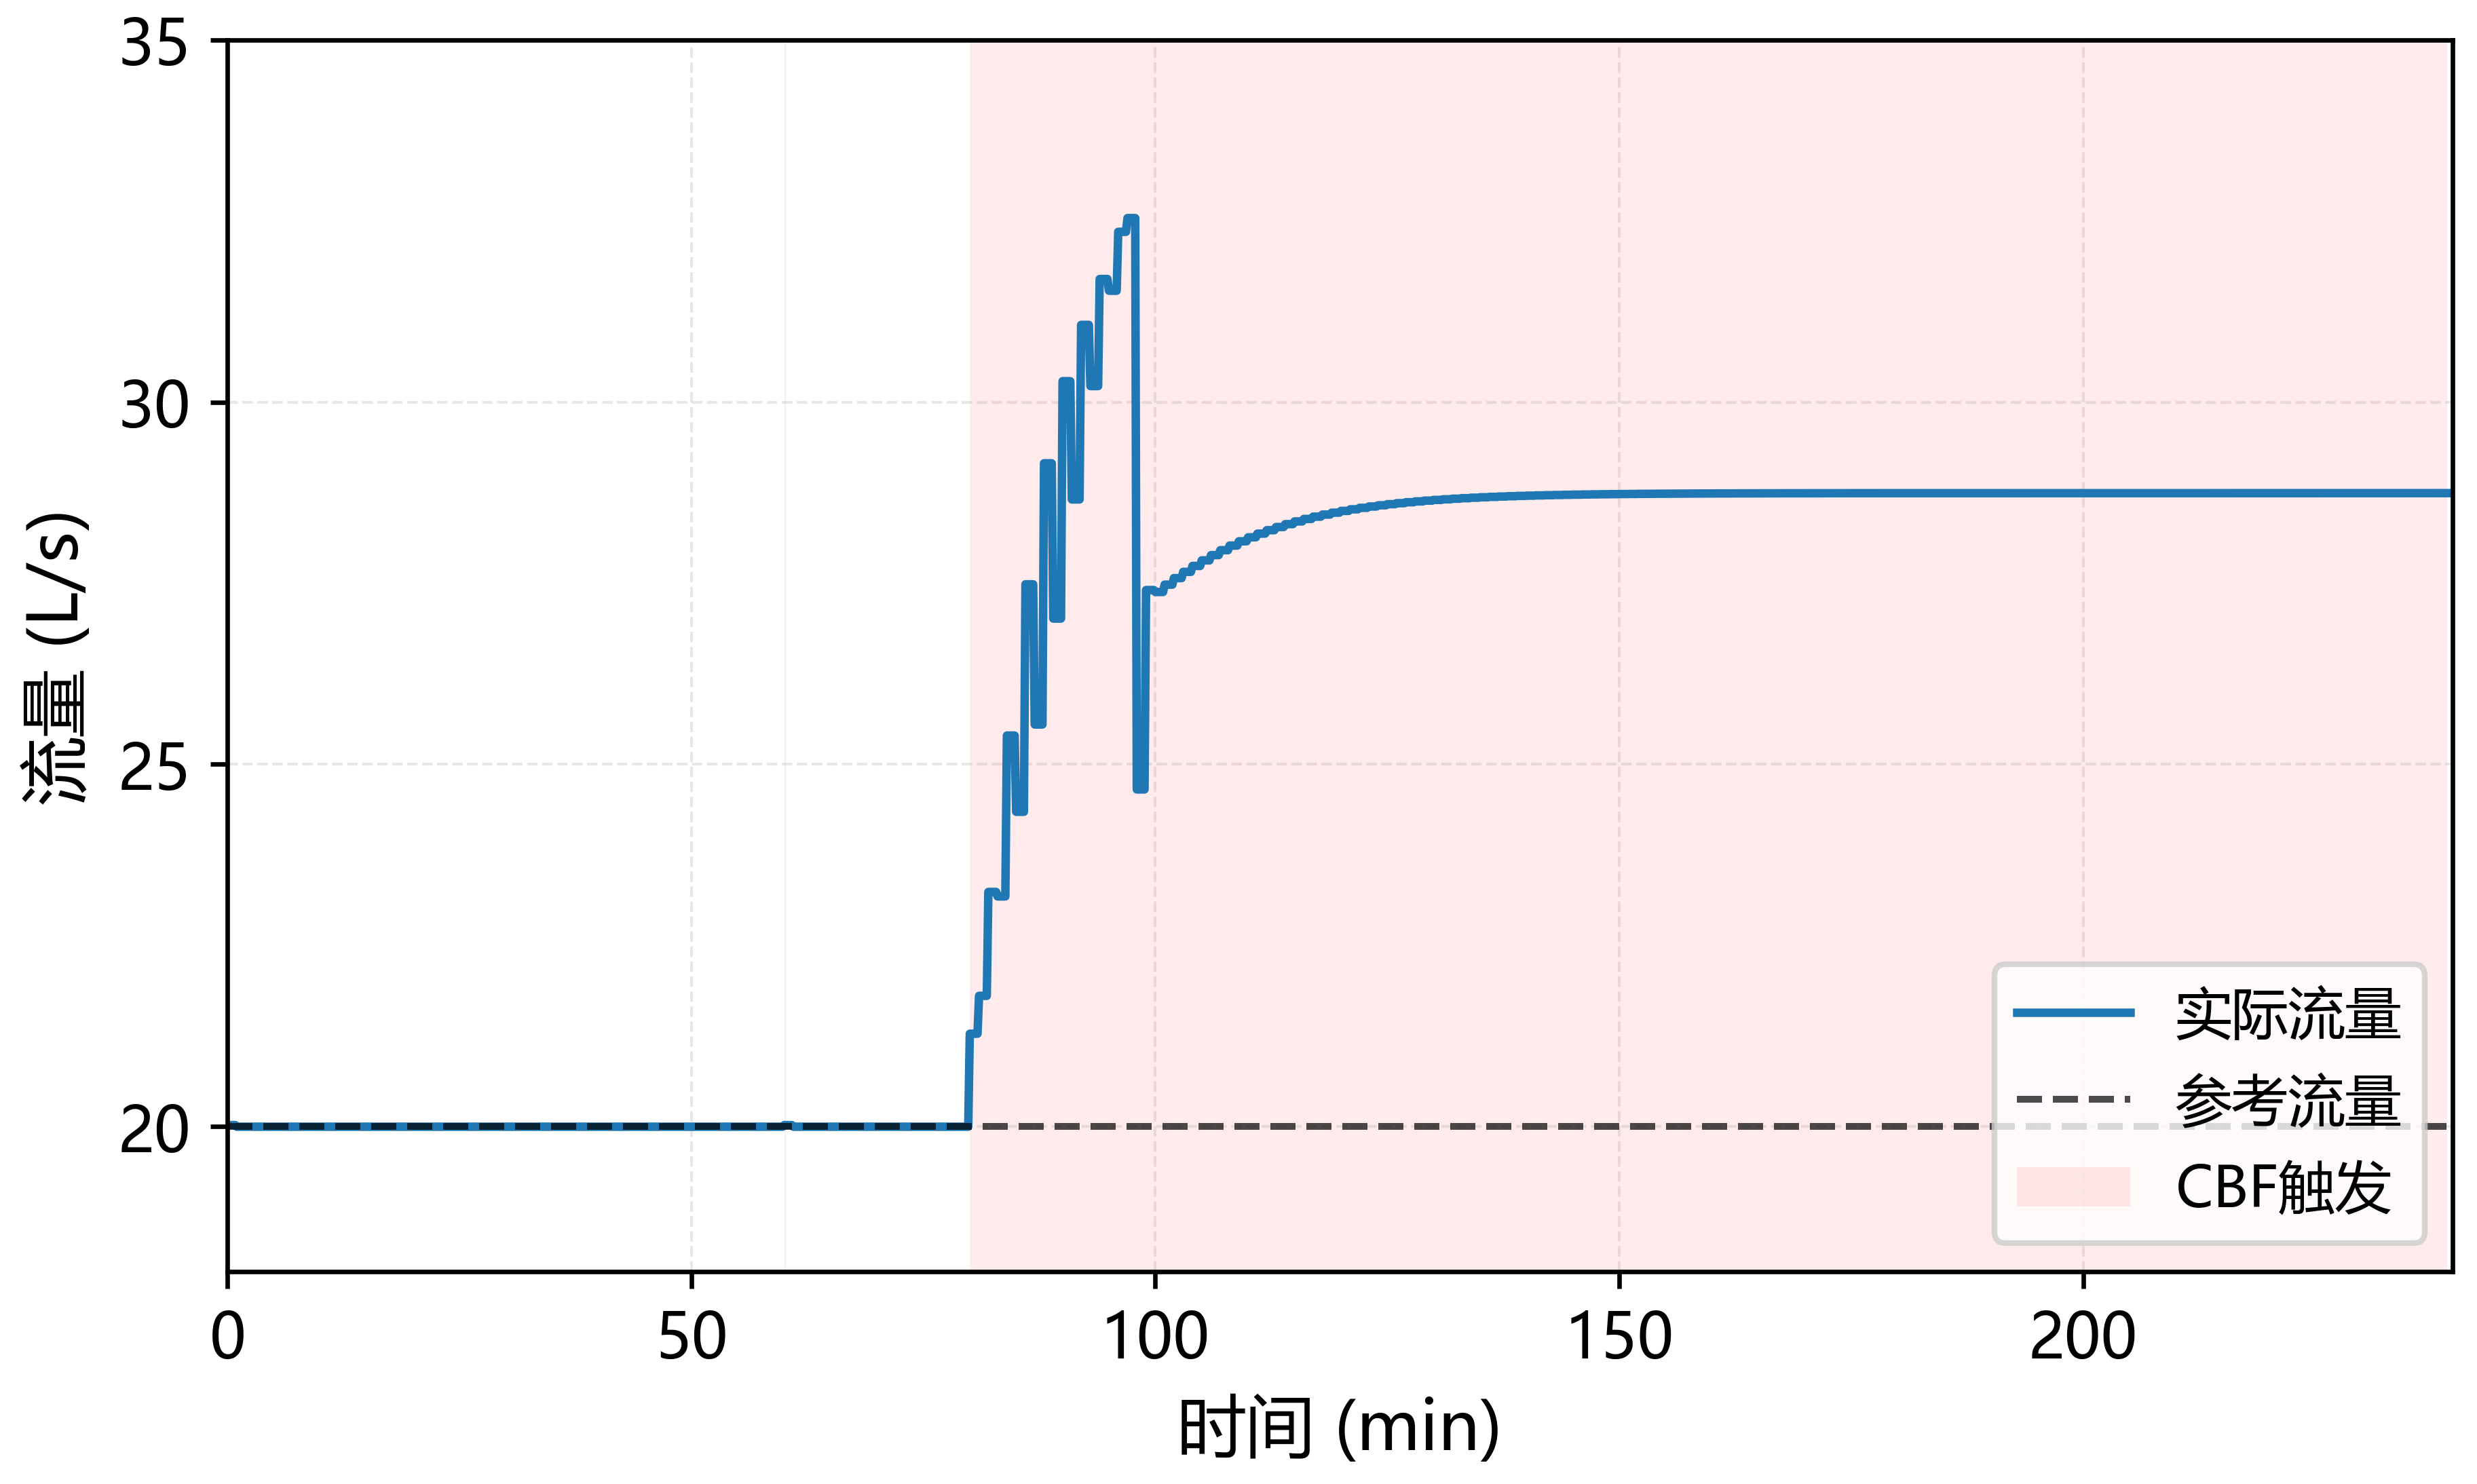
\includegraphics[width=\linewidth]{figures/cbf_temp_protection_c.png}
    \caption{}
  \end{subfigure}
  \hfill
  \begin{subfigure}{0.48\textwidth}
    \centering
    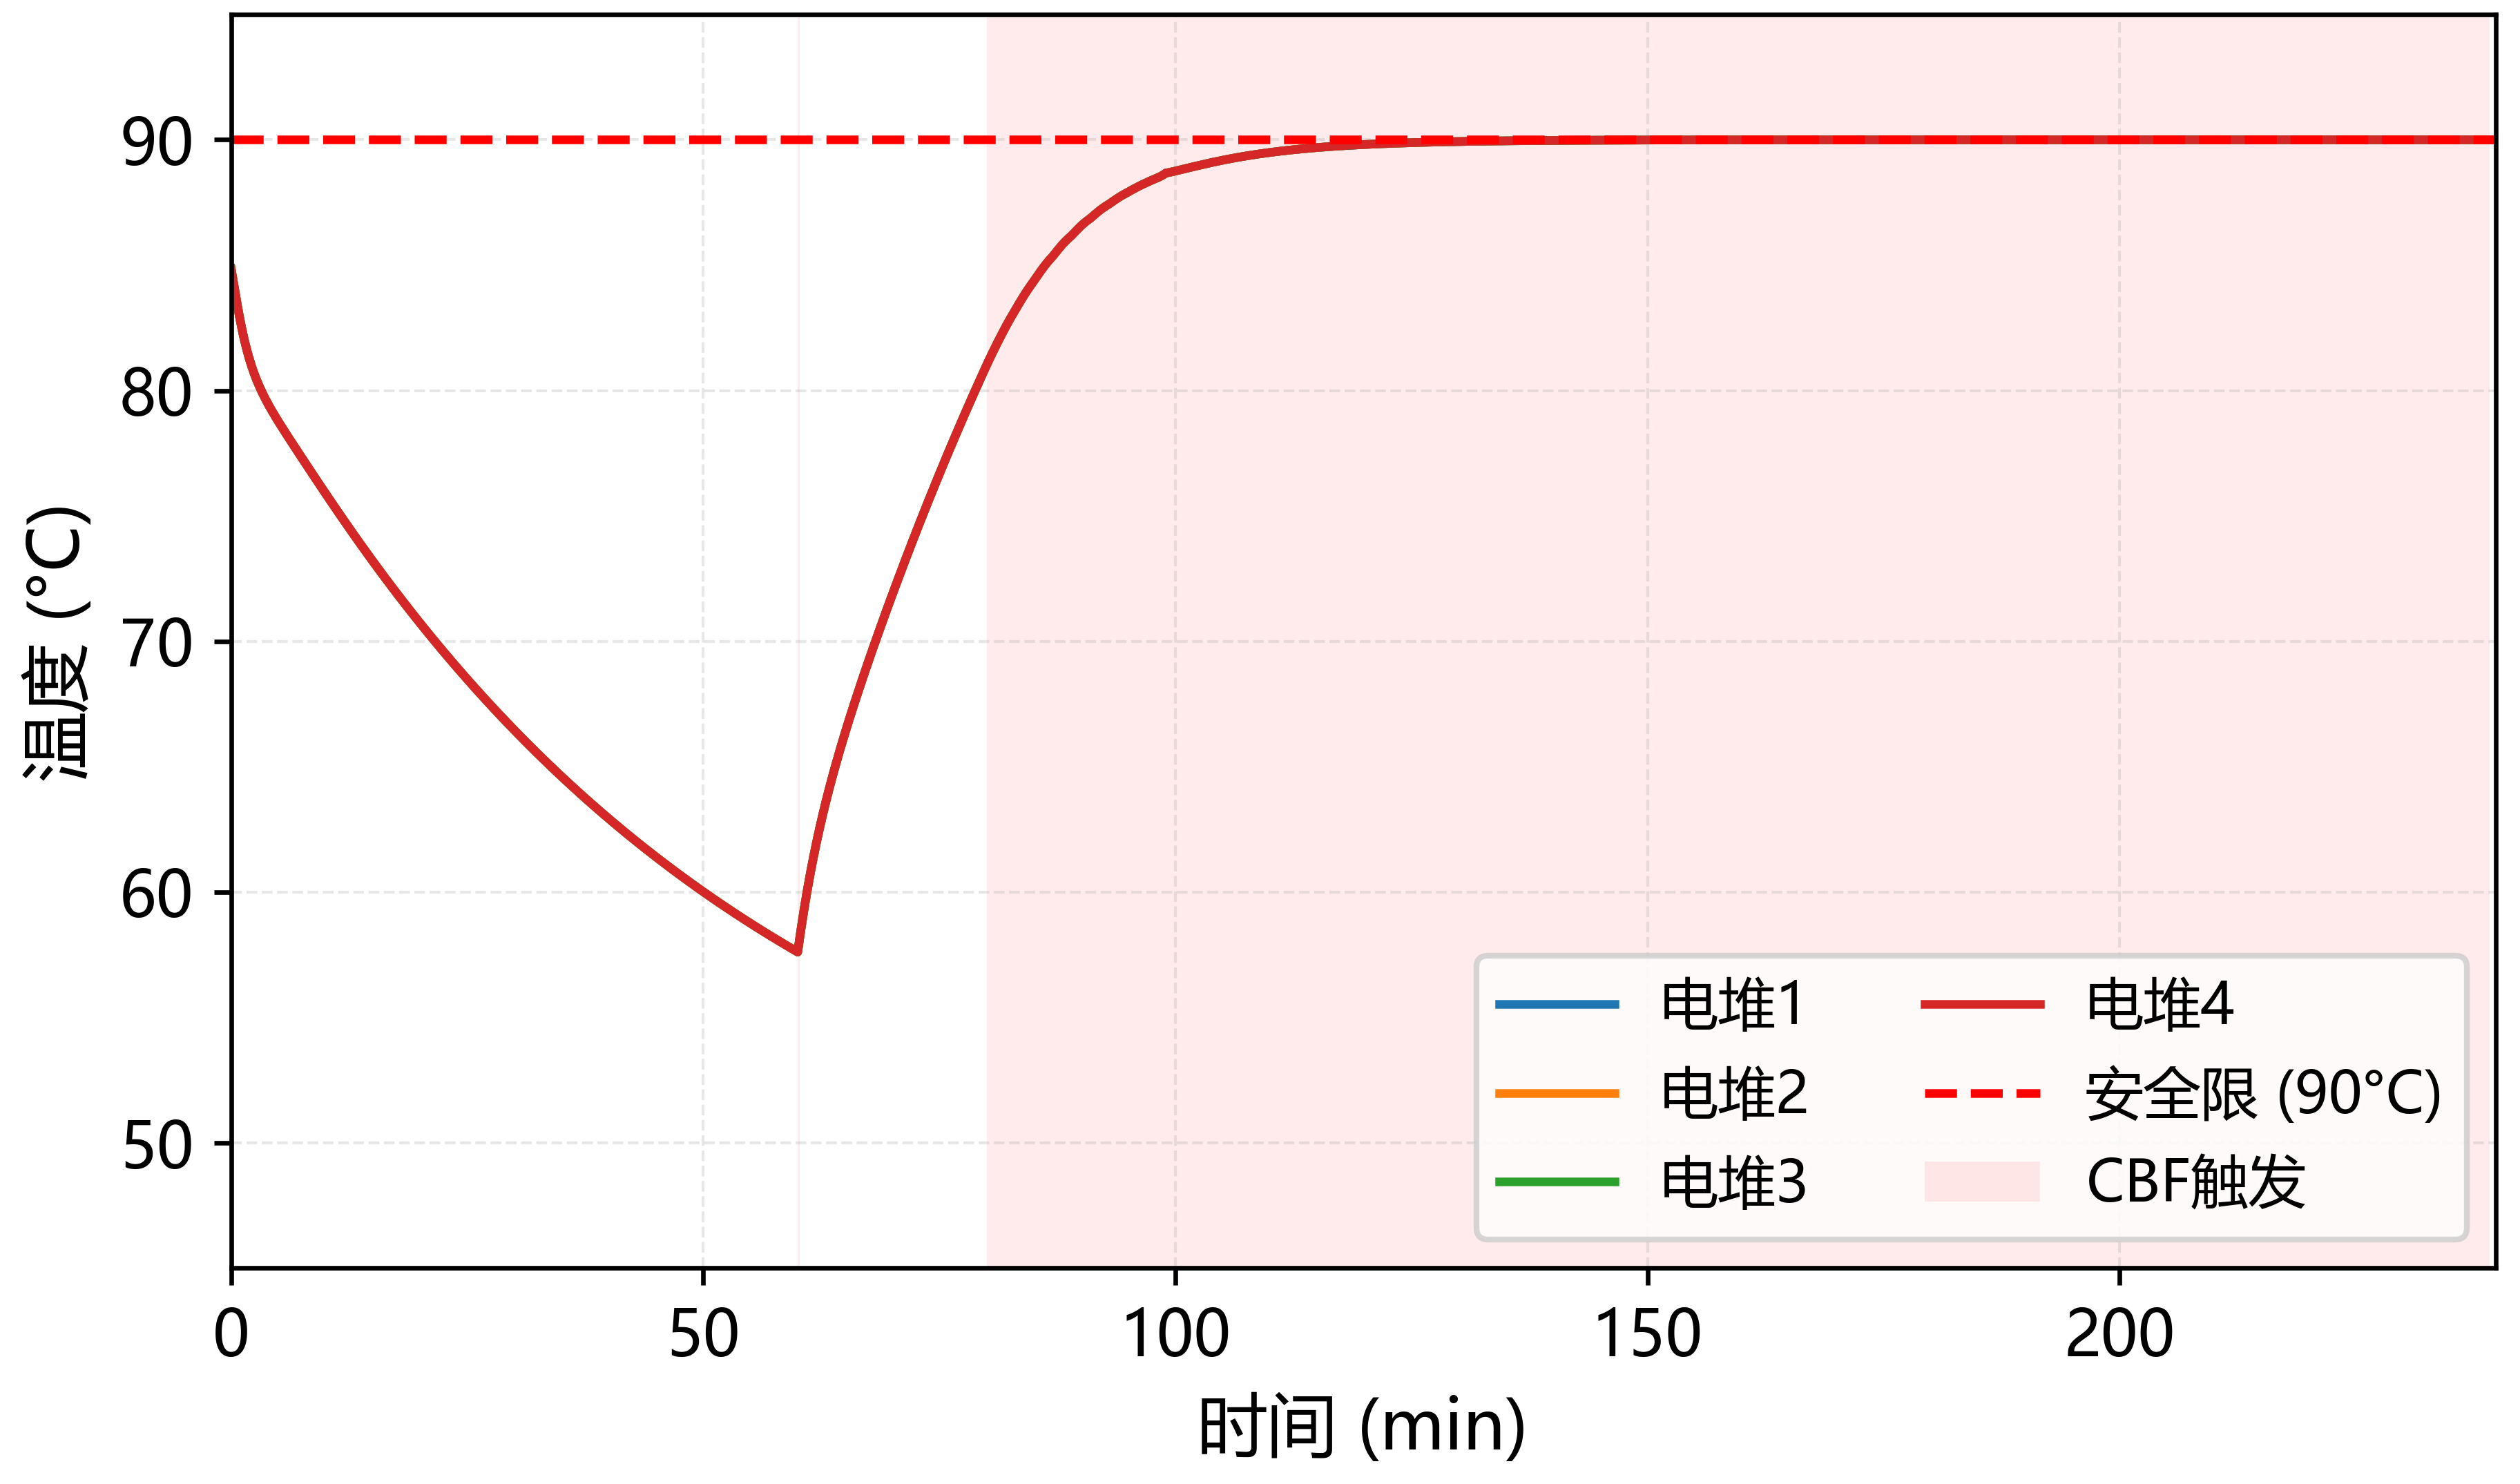
\includegraphics[width=\linewidth]{figures/cbf_temp_protection_d.png}
    \caption{}
  \end{subfigure}
  \caption{多重CBF联合约束闭环验证结果（高温约束保护工况）}
  \captionsetup{font=normalfont}
  \caption*{(a) 电解槽电流；(b) 碱液流量；(c) 冷却水流量；(d) 温度安全控制}
  \label{fig:cbf_temp_protection}
\end{figure}


\subsubsection{高功率温度保护实验}

系统初始运行于3000~A稳态，$t=60$~min时刻参考电流阶跃升至7500~A，模拟强产热极端工况。功率骤升导致电化学反应产热急剧增加，若不施加约束温度将迅速突破90$^\circ$C上限。CBF参数与场景一保持一致。

图~\ref{fig:cbf_temp_protection} 展示了闭环验证结果。电流阶跃后各槽温度明显上升，CBF在温度接近安全边界时及时触发（共162次，占11.3\%），通过主动增加冷却水流量（从20~L/s增至最高32.5~L/s）并适度调节电流，将温度严格控制在90$^\circ$C边界（最高90.00$^\circ$C）。HTO同步保持在2\%以内（峰值1.06\%）。该控制行为可由式~\eqref{eq:h1_dot} 解释：冷却水流量以仿射形式直接作用于热平衡动态，是降低温度灵敏度最高的控制通道，因此CBF优先大幅增大冷却水以快速带走反应热；电流则以非仿射项$\alpha(\mathbf{x}, u_1)$进入约束，且由$U_{cell} > \eta_F U_{th}$可知增大电流恒导致产热增加，故CBF仅适度调节电流以避免热负荷进一步恶化。温度约束采用一阶CBF即可获得平滑且迅速的冷却水响应，验证了CBF安全滤波框架在高温约束保护工况下的有效性。

综合两个场景可见：低功率工况下HTO约束主导安全边界，一阶CBF通过碱液流量的直接调节抑制氢气累积，将HTO严格控制在安全限以内；高功率工况下温度约束主导，一阶CBF通过冷却水流量的快速响应控制热平衡。两种极端工况分别验证了多重CBF联合约束框架在不同主导约束下的安全保证能力，且单次求解均满足实时控制要求。

